\documentclass{report} % either that or scrreprt

%% chapters 
\usepackage[Glenn]{fncychap}
%Sonny, Lenny, Glenn, Conny, Rejne, Bjarne, and Bjornstrup

\usepackage{graphbox,graphicx}
\usepackage{mathtools}
\usepackage{xcolor}
\usepackage{tikz}
\usepackage[most]{tcolorbox}
\usepackage{listings}

\definecolor{codegreen}{rgb}{0,0.6,0}
\definecolor{codegray}{rgb}{0.5,0.5,0.5}
\definecolor{awesome}{rgb}{1.0, 0.13, 0.32}
\definecolor{codepurple}{rgb}{0.58,0,0.82}
\definecolor{backcolour}{rgb}{0.95,0.95,0.92}

\lstdefinestyle{mystyle}{
    backgroundcolor=\color{backcolour},   
    commentstyle=\color{codegreen},
    keywordstyle=\color{magenta},
    numberstyle=\tiny\color{codegray},
    stringstyle=\color{codepurple},
    basicstyle=\ttfamily\footnotesize,
    breakatwhitespace=false,         
    breaklines=true,                 
    captionpos=b,                    
    keepspaces=true,                 
    numbers=left,                    
    numbersep=5pt,                  
    showspaces=false,                
    showstringspaces=false,
    showtabs=false,                  
    tabsize=2
}
\lstset{style=mystyle}



\usepackage{booktabs,caption}
\usepackage[flushleft]{threeparttable}

\newtcbtheorem{post}
    {Postulado}{}{theorem}
\newtcbtheorem{theo}
    {Teorema}{}{theorem}

\definecolor{dark green}{rgb}{0.0, 0.42, 0.24}
\usepackage{subfig}
% \usepackage{arsclassica}
% \usepackage{scrlayer-scrpage}
% \usepackage[sort&compress,numbers]{natbib}
\usepackage[spanish]{babel}
\usepackage[right=2cm,left=3cm,top=2cm,bottom=2cm,headsep=0cm,footskip=0.5cm]{geometry}
\usepackage{physics}
\ifpdf
\usepackage{pdfcolmk}
\usepackage{fixmath}
\fi
\usepackage{ulem}
%% check if using xelatex rather than pdflatex

\usepackage{breqn}
\usepackage{blindtext}
\usepackage[T1]{fontenc}
\usepackage{graphicx}
\usepackage{tikz}
\usepackage[toc]{appendix} 
\usepackage{comment}
\excludecomment{Omitir}

\usepackage{xcolor}
\newcommand{\notamm}[1]{{\color{orange} [Comentario MM: #1]}}
\newcommand{\notaFTBP}[1]{{\color{blue} [Comentario FTBP: #1]}}

\usepackage{tabularx} 
\usepackage{textcomp}
\usepackage{amssymb} 
\usepackage[utf8]{inputenc}
\usepackage{stackengine}
\usepackage{dsfont}
\usepackage{cancel}
\usepackage{fancyvrb}
\usepackage{amsmath}
\usepackage{amsthm}
\usepackage{epstopdf}
\usepackage{inputenc}
\usepackage{blindtext}
\usepackage[arrow]{hhtensor}  
\usepackage{slashed}
\usepackage{hyperref} 
\usepackage{multirow}
\usepackage{tabularx,colortbl}
\newcommand{\cronoentry}[1]{\begin{minipage}{7cm}\vspace{.1cm}#1 \\  \end{minipage}}
\DeclareOldFontCommand{\bf}{\normalfont\bfseries}{\mathbf}

\ifpdf
\usepackage{pdfcolmk}
\fi
\ifxetex
\usepackage{fontspec}
\fi
\providecommand{\HUGE}{\Huge}% if not using memoir
\newlength{\drop}% for my convenience
%% specify the Webomints family
% \newcommand*{\wb}[1]{\fontsize{#1}{#2}\usefont{U}{webo}{xl}{n}}
%% select a (FontSite) font by its font family ID
\newcommand*{\FSfont}[1]{\fontencoding{T1}\fontfamily{#1}\selectfont}
%% if you don’t have the FontSite fonts either \renewcommand*{\FSfont}[1]{}
%% or use your own choice of family.
%% select a (TeX Font) font by its font family ID
\newcommand*{\TXfont}[1]{\fontencoding{T1}\fontfamily{#1}\selectfont}
%% Generic publisher’s logo

\definecolor{skyblue}{rgb}{0.53, 0.81, 0.92}
\definecolor{Dark}{gray}{0.2}
\definecolor{MedDark}{gray}{0.4}
\definecolor{Medium}{gray}{0.6}
\definecolor{Light}{gray}{0.8}
\hypersetup{
colorlinks=true,
    breaklinks=true,
	linkcolor=blue,    
	citecolor=red,       
	filecolor=magenta,     
	urlcolor=red         }
\geometry{left=2.5cm,right=2.5cm,top=2.5cm,bottom=2.5cm}
\usepackage{cite} 
\newtheorem{theorem}{Teorema}[section]
\newtheorem{corollary}{Corolario}[theorem]
\newtheorem{definition}{Definición}[section]
\newcommand{\sii}{\textit{sii }}
\newcommand{\R}{\mathbb{R}}
\newcommand{\lgg}{\langle}
\newcommand{\rgg}{\rangle}
\newcommand{\eg}{\textit{eg. }}
\newcommand{\ie}{\textit{ie. }}
\newcommand{\ansatz}{\textit{ansatz} }

\usepackage{comment}
\excludecomment{excluir}

\newcommand{\titleLLL}{
\begin{center}
\vspace*{1cm}
       \textcolor{Dark}{\HUGE \bf Simulación eficiente de dinámicas \\
       no markovianas mediante estados Max-Ent}
       
       \vspace{2cm}
        {\Large Federico Tom\'as P\'erez}\par
        \vspace{0.5cm}
        {\Large Director: Dr. Juan Mauricio         Matera}\par\vspace{0.5cm}
        {\Large Asesora académica: Prof. Dra. Norma       Canosa}\par 
        \vspace{2cm}
        {\Large Mesa Jurada conformada por el Dr. Juan        Mauricio Matera, la Prof. Dra. Norma Canosa y      la Prof. Dra. Marta Reboiro }

\vspace{2cm}
            
       \vfill
       Tesis de Licenciatura para optar el título de grado de Licenciado en Física
        
       \vspace{0.8cm}
     
       
\includegraphics[width=5cm]{escudo-UNLP_color.jpg}
       
       Departmento de Física de La Plata \\
       Facultad de Ciencias Exactas, \\
       Universidad Nacional de La Plata\\
       La Plata, Pcia. de Buenos Aires, Argentina\\
       \today
       \end{center}
}
\newcommand{\titleLL}{
\pagestyle{empty}
\begingroup% Lost Languages
\drop=0.1\textheight
\fboxsep 0.9\baselineskip
\sffamily
\vspace*{\drop}
\centering
{\textcolor{Dark}{\HUGE \bf Simulación eficiente de 
dinámicas no
markovianas 
mediante estados Max-Ent}}\par
%\vspace{0.5 \drop}

\vfill
{\small La Plata, \today \\ 
\includegraphics[width=5cm]{escudo-UNLP.jpg}}\par
\vspace*{.2\drop}
{\Large Tom\'as P\'erez}\par
\vspace{.2\drop}
{\Large Director: Dr. Juan Mauricio Matera}\par\vspace*{.1\drop}
{\Large Asesora académica: Prof. Dra. Norma Canosa}\par 
\vspace{.2\drop}
{\Large Mesa Jurada conformada por el Dr. Juan Mauricio Matera, la Prof. Dra. Norma Canosa y la Prof. Dra. Marta Reboiro }

\vspace{.2\drop}
{\medium Requerimiento para optar el título de Licenciado en Física}
%\vspace*{.25\drop}
\vfill

%\vspace{0.25\drop}
%{\Large Investigador Adjunto}\par

\vspace*{\drop}
\endgroup
\clearpage
\hspace{1cm}
\newpage
\pagestyle{plain}
}
\numberwithin{equation}{section}
\begin{document}
\titleLLL
\newpage

\vspace*{\fill}
{\Large Soporte externo}

\textnormal{  }\newline

\noindent El código fuente de las simulaciones y cálculos numéricos implementados en este trabajo de diploma se encuentran disponibles en \href{https://github.com/licTomasPerez/-Code-Thesis-Non-markovian-Dynamics}{Github}. El archivo fuente de la presente tesis se encuentra disponible en \href{https://github.com/licTomasPerez/Thesis-Efficient-simulation-of-non-markovian-dynamics-using-Max-Ent-states-}{Github}.

En el presente trabajo utilizaremos el sistema de unidades naturales $\hbar = c = 1$. \\

{Contacto}: \href{mailto:tomasemperador01@gmail.com}{tomasemperador01@gmail.com.}

\newpage\null\thispagestyle{empty}\newpage

\tableofcontents
\newpage

\section*{Resumen}

\noindent En el presente trabajo estudiaremos el problema de resolución de la dinámica de un sistema cuántico no markoviano multipartito mediante las ecuaciones de Schrödinger y Lindblad, un problema de complejidad algorítmica \textbf{NP-hard}, mediante la aproximación de los estados instantáneos por estados tipo \textbf{Max-Ent} con correlaciones de hasta dos cuerpos, un problema de complejidad \textit{a priori} \textbf{P}. A tal fin, se usó el formalismo de \textbf{dinámicas Gaussianas} para dichos sistemas y se construyó un enfoque nuevo de dinámicas Gaussianas como una aplicación del Principio Max-Ent para la descripción de dinámicas abiertas y cerradas de sistemas cuánticos no markovianos.  

\vspace*{\fill}
{\Large \textbf{Abstract}}\newline

\noindent In this work we will study the problem of solving the Schrödinger and Lindblad equations for non-Markovian correlated multipartite quantum systems, a problem of \textbf{NP-hard} algorithmic complexity, by the means of approximating the instantaneous states by \textbf{Max-Ent}-type states, counting only up to two-body correlations; \textit{a priori} a problem of \textbf{P} complexity. To that end, we implemented the \textbf{Gaussian dynamics} formalism for such systems and a new Gaussian dynamics approach as an application of the Max-Ent Principle for the description of open and closed dynamics for non-Markovian quantum systems. 
\newpage\null\thispagestyle{empty}\newpage

\chapter{Introducci\'on}

La investigación de la dinámica de sistemas cuánticos es fundamental para la comprensión y modelado de los fenómenos a escala nanoscópica, siendo especialmente relevante en los campos de estudio de medicina \cite{PCHP.10}, comunicaciones  \cite{Caldeira1981, Chirolli2008, Burkard2009, Tan2011}, en Física Atómica y Molecular y en Física de la Materia Condensada \cite{Zhou2017, Breuer2016,HOPS,TEDOPA,DAMPF,Farina2019}.

Al construir un modelo de cierto proceso físico, se han de tener en cuenta dos características físicamente significativas

\begin{enumerate}
    \item Los \underline{grados de libertad} accesibles al sistema, los cuales limitan el número de estados compatibles con los vínculos del sistema. Estos son las cantidades que pueden ser controladas o medidas \eg momento, posición, proyección de espín de una dada partícula etc.
    \item Las \underline{simetrías internas} de la teoría, que se traducirán en vínculos sobre la evolución temporal de cantidades físicas.
\end{enumerate}

Conociendo estas propiedades del sistema en cuestión, la mecánica cuántica establece un marco de trabajo para construir un modelo matemático que lo describa. Una estrategia útil para llegar a tal construcción es partir de identificar subcomponentes bien definidas en el sistema a describir, y sus posibles interacciones, análogamente a la dinámica clásica. Sin embargo, y a diferencia de lo que ocurre en la mecánica clásica, a la hora de describir el estado del sistema y su evolución, no será posible aplicar esta separación en componentes. Esto es debido a la existencia de observables incompatibles. Dicha incompatibilidad impide, en general, especificar el estado del sistema únicamente en términos de los estados de las partes que lo forman, sino que también se requiere de especificar las correlaciones entre ellas. 

Esto impone una dificultad al intentar describir sistemas de muchos componentes.
En general, para sistemas \textit{many-body} de $n$-subcomponentes, el espacio de Hilbert de los estados accesibles será del orden $\mathcal{O}(2^n)$-dimensional y el objeto matemático que lo describe tendrá $\mathcal{O}(2^{2n})$ elementos a especificar. Además el número de grados de libertad crecerá geométricamente, como también el número de posibles correlaciones - y por lo tanto de  cantidades a considerar - lo cual vuelve al tratamiento exacto un problema irresoluble -. Formalmente, esto implica que la resolución de la ecuación de Schrödinger es un problema \textbf{NP-hard} \cite{bolotin2013computational, bolotin2014computational}.

Los sistemas cuánticos de interés a este trabajo de diploma son sistemas con correlaciones y por tanto admiten una descripción mediante métodos matemáticos propios al análisis estocástico. Diremos que un \textbf{proceso estocástico} \cite{HeinzPetruccione} es una familia de variables aleatorias uni-parametrizadas 
por un número real. Luego, definiremos un \textbf{proceso de Markov} \cite{HeinzPetruccione} como un tipo especial de proceso estocástico, ya sea discreto o continuo, en el cual la probabilidad de un evento depende \textit{solamente} del evento inmediatamente anterior. Esto implica que la jerarquía de distribuciones de probabilidad conjunta pueden ser construidas con solo dos funciones de distribución. Esta condición de Markov simplifica substancialmente la descripción matemática de un proceso estocástico puesto que la evolución de la probabilidad de transición condicional asociada a un proceso de Markov clásico, en particular, está determinada por la ecuación de Chapman-Kolmogorov \cite{HeinzPetruccione, Dynkin89}; no existiendo su análogo para un proceso de Markov cuántico. En particular, en este trabajo, nos interesará estudiar sistemas \textbf{No-Markovianos}: sistemas físicos que presentarán correlaciones no negligibles con el ambiente en que están inmersos a largo plazo que afectarán la evolución del sistema. 

Para el tratamiento de sistemas no-markovianos se han desarrollado diferentes aproximaciones y formalismos tales como los mapeos bosónicos \cite{huber2020phase}, representaciones en tensor networks \cite{HOPS,TEDOPA,DAMPF}, modelos basados en dinámicas de saltos cuánticos \cite{Plenio1998,Pilo2008}, entre otros. Cada uno de estos formalismos se basan en volver tratable el problema haciendo algunas hipótesis sobre la forma de las correlaciones que desarrollará el sistema en su evolución. 

En la práctica, muchas veces es posible despreciar, en una primera aproximación, el efecto de las correlaciones y de las interacciones que las producen. Cuando esto es posible, la dinámica del estado de cada constituyente se desacopla en un conjunto de problemas locales, lo que vuelve a la simulación un problema resoluble. En esta idea, se basan las llamadas \textbf{Teorías de campo medio dinámicas} \cite{GKW1996}. Usando este tipo de estrategias, es posible incluso tener en cuenta algunos tipos de correlaciones clásicas\cite{CMR.07}. 

En muchas otras situaciones, sin embargo, es importante tener en cuenta los efectos de las correlaciones - o bien por tratarse de un régimen no perturbativo -, o bien porque lo que se busca determinar es la existencia y magnitud de las correlaciones cuánticas- de forma tal que los métodos que desprecian las correlaciones no son adecuados para el tratamiento de dicho sistema. 

Una estrategia que permite estudiar sistemas con correlaciones consiste en el uso de los \textbf{estados Gaussianos}. Los estados Gaussianos son una familia de estados térmicos, obtenidos mediante la exponenciación de una forma cuadrática definida positiva afín en operadores de creación y destrucción fermiónicos o bosónicos. Esto permite construir clases de equivalencia de estados de Gibbs \cite{PATHRIA2011115} \ie la exponencial de un Hamiltoniano, en el que los operadores asociados a los observables de correlación se traducen en una interacción efectiva de ese Hamiltoniano. Resulta que las dinámicas gaussianas son parametrizables en términos de sus correlaciones de pares, lo cual será útil a la hora de construir una variedad diferenciable Riemanniana \cite{NakaharaM} de dichos estados, lo cual será discutido en el \autoref{Appendix A}.

En un sistema con correlaciones gaussianas, el valor medio de cualquier observable queda determinado en términos de los valores medios locales y las correlaciones de pares de un cierto conjunto de operadores locales, que juegan un papel análogo a los de las coordenadas e impulsos en un sistema de osciladores armónicos acoplados. Los estados gaussianos son muy útiles ya que, a la vez de soportar correlaciones cuánticas,  proveen de un modelo efectivo simple e intuitivo para el sistema original, lo que contribuye a interpretar fácilmente los resultados obtenidos.

Si un sistema bosónico se encuentra inicialmente en un estado gaussiano, y su dinámica está gobernada por una ecuación de Schr\"odinger con un Hamiltoniano cuadrático en los operadores de creación y aniquilación, es posible ver que el estado del sistema continuará siendo Gaussiano en todo momento posterior. Lo mismo vale en el caso de dinámicas abiertas cuando los operadores de colapso son lineales en estos operadores, Esto se discutirá en mayor detalle en el \autoref{ApendixA}. Esto permite reducir el problema de la dinámica en sistemas gaussianos al problema de la dinámica de sus correlaciones de pares, lo que vuelve resoluble en forma eficiente a sistemas con una cantidad moderadamente grande de componentes \cite{Feynman1963,Illuminati2018}. Esto ha motivado buscar esquemas que generalicen estos resultados a sistemas más complejos mediante el formalismo de mapeos bosónicos y en desarrollar diferentes estrategias de mapeo, así como en generalizar las correlaciones gaussianas a correlaciones soportadas en sistemas más generales.

La limitación implícita en esta estrategia es que, aún en el régimen de correlaciones pequeñas, muchos sistemas de interés no  cumplen la condición de gaussianidad. Por ejemplo, cualquier sistema con espacios de estados locales de dimensión finita, dejan de ser gaussianos en el régimen de altas temperaturas. En la figura \ref{Aproximacion Gaussiana} se muestra un esquema de la aplicabilidad de la aproximación gaussiana para un sistema físico compuesto de dos subsistemas de espín 1/2 \footnote{En este ejemplo, se analiza la aplicabilidad de un mapeo bosónico entre un sistema de dos espines acoplados y un sistema de dos osciladores armónicos acoplados. En general, este mapeo está dado en términos de una \textit{transformación de Jordan-Wigner} \cite{Nielsen.00}, mientras que el mapeo inverso que recupera la situación original está dado por una \textit{transformación de Klein} \cite{ringwood}, automorfismos entre álgebras bosónicas y automorfismos entre álgebras fermiónicas.}. En un régimen de bajas temperaturas y correlaciones pequeñas, la aproximación gaussiana es un formalismo útil; no siendo esto verdadero para el régimen de altas temperaturas y correlaciones grandes. 
\begin{figure}
    \centering
    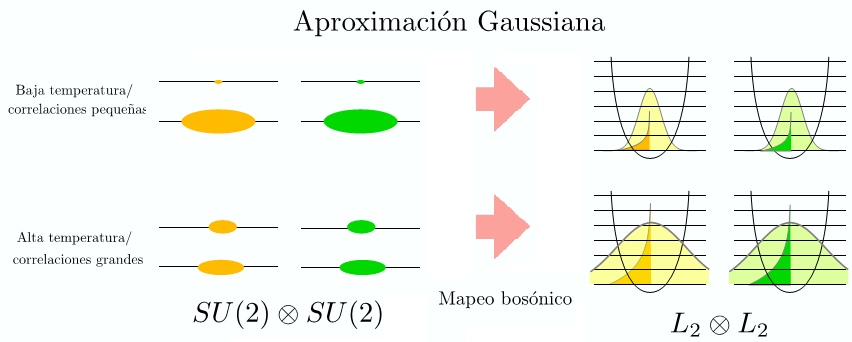
\includegraphics[scale = 0.57]{figs/Aproximacion Gaussiana.png}
    \caption{En el presente diagrama se muestra un esquema de la aproximación gaussiana a un sistema con un acoplamiento de dos subsistemas de espín $\frac{1}{2}$. En el régimen de bajas temperaturas y correlaciones pequeñas, es posible construir un mapeo bosónico a un sistema de dos osciladores armónicos acoplados el cual es una aproximación fidedigna al sistema original, esto es los observables físicos relevantes calculados para el sistema bosónico son afines a aquellos resultados obtenidos para el sistema original. Por ejemplo, el número de ocupación para el sistema bosónico sólo será significativo para el estado fundamental y el primer excitado, siendo negligible para el resto. Sin embargo, en el régimen de altas temperaturas, este formalismo se vuelve inaplicable puesto que las correlaciones se vuelven cada vez más significativas y afectan más los resultados.}
    \label{Aproximacion Gaussiana}
\end{figure}

En este trabajo proponemos atacar el problema de la gaussianización desde una perspectiva diferente, basada en la propiedad \textbf{Max-Ent} de los estados Gaussianos \cite{Jaynes1, Jaynes2,RP.89,rossignoli1990extmf}. Esta propiedad consiste en ser estados que maximizan la entrop\'ia de von Neumann sobre todos los posibles estados que reproducen los mismos valores medios para ciertos observables, que en el caso gaussiano son las correlaciones de pares y los observables de un cuerpo \cite{Nielsen.00}.

En este trabajo, proponemos entonces utilizar esta propiedad para \emph{gaussianizar} en forma implícita sistemas que no necesariamente están constituídos por modos bosónicos
y explorar aplicaciones de esta estrategia a dinámicas en sistemas bosónicos y sistemas de espines interactuantes. Mediante la elección apropiada de familias de estados Max-Ent, buscaremos representar de forma eficiente y precisa los estados correspondientes a la dinámica exacta de sistemas estos sistemas de interés actual. 

\section*{Plan de la obra}

%\st{En el presente trabajo, se utilizar\'a el principio Max-Ent y el formalismo de din\'amicas Gaussianas para modelar la din\'amica cerrada y abierta para diversos sistemas cu\'anticos de m\'ultiples subcomponentes no markovianos.}
%\st{Entre ellos, estudiaremos modelos de sistemas de dos componentes bos\'onicas y modelos con acoplamiento esp\'in-bos\'on.}
%\st{Se har\'a uso de la biblioteca \textbf{QuTip} del lenguaje Python para simular num\'ericamente la din\'amica de dichos sistemas
%}\st{cu\'anticos y cotejar los resultados anal\'iticos con los resultados num\'ericos, buscando estudiar la efectividad y}
%\st{ viabilidad de obtener resultados fidedignos mediante la aproximaci\'on por estados instant\'aneos tipo Max-Ent. }

En el presente trabajo, se utilizará el Principio Max-Ent y el formalismo de dinámicas Gaussianas para modelar las dinámicas cerradas y abiertas de distintos sistemas, tanto markovianos como no markovianos.

En el \autoref{cap3_dosbosones} se explican las bases de la Mecánica Cuántica, el formalismo Markoviano de ecuaciones Maestras de Lindblad y el formalismo de dinámicas Gaussianas.

En el capítulo \autoref{chap3_dingauss} se usa el formalismo de dinámicas Gaussianas y el formalismo de ecuaciones maestras de Lindblad para estudiar distintas evoluciones de un sistema de dos subsistemas bosónicos acoplados, comparando los resultados analíticos con resultados numéricos con el fin de analizar la aplicabilidad de los formalismos empleados.

En el capítulo \autoref{chap4_allmaxent} se explica la base del formalismo Max-Ent dándo un enfoque nuevo a las dinámicas Gaussianas para la descripción de sistemas no markovianos. Se explican diversas rutinas numéricas implementadas, destacando en particular un método novedoso de Proyección ortogonal. 

A continuación, en el capítulo \autoref{chapter5}
se estudian diversas aplicaciones de los formalismos anteriores en la descripción de dinámicas tanto gaussianas y cuasi-gaussianas como no gaussianas para sistemas bosónicos y espinoriales, buscando analizar la efectividad y aplicabilidad de los formalismos anteriores. 

En el capítulo \autoref{Chapter6} se analizan las conclusiones de los resultados derivados anteriormente como también se presenta un plan para futuros desarrollos. Asimismo, el trabajo presenta cuatro apéndices. En el \autoref{Appendix A} se discuten algunos detalles matemáticos adicionales de importancia a este trabajo, en los \autoref{ApendixA} y \autoref{AppendixB} se estudian algunas propiedades generales de sistemas bosónicos y se explican los algoritmos implementados en este trabajo respectivamente y finalmente en el \autoref{Appendix D} se presenta y se discute el código y algoritmo elaborado y estudiado en este trabajo. 

\newpage\null\thispagestyle{empty}\newpage

\chapter{Modelado de sistemas cu\'anticos }
\label{chapter2}

\section{Postulados de la mec\'anica cu\'antica}

La base matemática de la mecánica cuántica se halla en el teorema espectral  \cite{HoracioI,HeinzPetruccione,BCHallp} y la correspondencia entre observables físicos y operadores auto-adjuntos. Dicha teoría encuentra su fundamento en una serie de postulados axiomáticos \cite{CohenTannoudji1989, Nielsen.00, HeinzPetruccione, Portesi-ECI34, Holik-ECI34}, los cuales pasaremos a enunciar en el presente capítulo.

\begin{post}{Sobre el espacio de estados}{Post state space}
Sea un sistema físico \underline{aislado} -esto es, no tiene interacciones con otros elementos por fuera del sistema en estudio-, existe un espacio vectorial complejo asociado a este sistema, provisto de un producto interno; el cual es completo y separable \ie un espacio de Hilbert equipado \cite{Nielsen.00, NakaharaM} denotado por $\mathbb{H}$. En este espacio se encuentran todos los \textbf{vectores de estado} que caracterizan el sistema. Diremos que $\mathbb{H}$ es el \textbf{espacio de estados}. 
\label{Post state space}
\end{post}

Las cantidades medibles y físicamente relevantes de un sistema físico son los \textbf{observables}. En el formalismo de la mecánica cuántica, los observables son representados por operadores lineales autoadjuntos sobre el espacio de Hilbert. Los resultados medibles serán los autovalores de dichos operadores autoadjuntos - que serán necesariamente reales - acorde al teorema de descomposición espectral.

Como buscamos estudiar sistemas con un gran número de partículas, hemos de recurrir a la \textit{mecánica estadística cuántica} \cite{PATHRIA2011115,Nielsen.00,HeinzPetruccione}. 
En esta teoría se introduce a la \textbf{matriz densidad} u \textbf{operador densidad}, denotado por $\rho$, el cual caracterizará completamente el estado del sistema. Este {operador densidad} $\rho$ es un operador hermítico, de traza unimodular y con todos sus autovalores no negativos; esto es
\begin{subequations}
\begin{align}
    \rho^{\dagger} = \rho, \\
    \Tr \rho = 1, \\
    \rho \geq 0.
\end{align}
\end{subequations}

Notemos que el conjunto de todas las matrices densidad es convexo, por lo que dadas cualesquiera matrices densidad $\rho_1, \rho_2$ luego $\rho = \lambda\rho_1+ (1-\lambda)\rho_2, \lambda \in \mathds{R}_{[0,1]}$ también es un estado densidad. Dicho conjunto de estados densidad $\mathcal{C}(\mathds{H})$ tiene \textit{a priori} la estructura de un espacio vectorial, con las operaciones usuales, sobre el cuerpo $\mathds{C}$, definido como 

\begin{equation}
    \mathcal{C}(\mathds{H}) = \{\rho \in GL(n, \mathds{C}) \textnormal{ }| \textnormal{ }\rho^{\dagger} = \rho \textnormal{, } \Tr \rho = 1 \textnormal{, } \rho \geq 0\},
\end{equation}

donde $GL(n,\mathds{C})$ es el conocido grupo lineal general sobre el cuerpo de los números complejos cuyos elementos son matrices de $\mathds{C}^{n\times n}$, descripción válida para un espacio de Hilbert finito-dimensional. En el \autoref{Appendix A} se incluyen algunas consideraciones teóricas adicionales y en la \autoref{hausdorff} se estudiará la estructura topológica de dicho espacio $\mathcal{C}(\mathds{H})$, demostrando que este espacio es una variedad Riemanniana. La formulación de la mecánica cuántica basada en el operador densidad como objeto de estudio es ideal para la descripción de subsistemas individuales de un sistema cuántico compuesto \cite{Nielsen.00} cuando los estados de dichos subsistemas no son completamente conocidos. \\

Sea un sistema cuántico con un espacio de Hilbert $\mathds{H}$ finito dimensional. Su estado se encuentra determinado por un ensamble estadístico \cite{Nielsen.00, PATHRIA2011115} $\mathcal{E} = \{p_i,\ket{i}\}_{i=1}^{n}$, donde $p_i \in \mathds{R}_{+}$ son, \textit{a priori}, los pesos de los estados - compatibles con los vínculos del sistema - de dicho ensamble $\mathcal{E}$. Este ensamble es, en esencia, un catálogo de probabilidades para cada resultado posible de una medida. En tales condiciones, y usando teoría de la medida, podemos definir algunos elementos importantes a la teoría,

\begin{itemize}
    \item primero, el espacio topológico $\mathcal{C}(\mathds{H})$ ya definido,
    \item una $\sigma$-álgebra $\mathcal{X}$. Dado que  $\mathcal{C}(\mathds{H})$ es un espacio topológico, sobre el cual es posible distinguir elementos, la elección natural de $\sigma$-álgebra es la $\sigma$-álgebra de Borel de dicho espacio: $\mathcal{X} = \mathcal{B}(\mathcal{C}(\mathds{H}))$
    \item y una medida de probabilidad $\mathds{P}$ bien definida sobre $\mathds{R}$, un espacio métrico, la cual cumple que $\mathds{P}(\mathcal{C}(\mathds{H})) = 1.$ Luego, $\mathds{P}: \mathcal{X} \rightarrow \mathds{R}_{[0,1]}$, 
\end{itemize}

Luego, en tales condiciones, el triple $(\Omega, \mathcal{X}, \mathds{P})$ es un espacio probabilístico \cite{Bartle1995, munkres}, sobre el cual se puede definir una variable aleatoria $\mathbf{X}: \Omega \rightarrow \mathds{R}$ que describe las probabilidades y resultados posibles al medir el estado $\rho$ en dicho ensamble de estados. Esto es, la probabilidad de medir el resultado $x_i$ es $\mathds{P}(x_i) = \Tr(\rho \Pi_i)$ \cite{HeinzPetruccione, Portesi-ECI34, Holik-ECI34}, acorde al teorema de Gleason\footnote{Formalmente, este teorema enuncia 

\begin{theo}{Teorema de Gleason}{}
Toda matriz densidad pura $\rho \in \mathcal{C}(\mathds{H})$ tiene una correspondencia biunívoca con una medida de probabilidad a valores reales $\mathds{P}: \mathcal{A} \rightarrow \mathds{R}_{[0,1]}$, para un espacio de Hilbert de dimensión mayor o igual a 3, tal que $\mathds{P}_{\rho} ({\bf A}) = \tr (\rho {\bf A})$ para todo observable ${\bf A}$.
\end{theo}
Adicionalmente se puede demostrar que las operaciones de traza y traza parcial son las únicas funciones de $\rho$ que modelan correctamente el comportamiento de sistemas cuánticos compuestos \cite{BE07}.} para cierto operador $\Pi_i$. Entonces la probabilidad de encontrar al sistema en un estado particular $\ket{\psi_i}$, normalizada al estar circunscrito a un espacio probabilístico, es

\begin{equation}
    p_i = \Tr (\rho \Pi_i) = \bra{\psi_i}\rho\ket{\psi_i},
\end{equation}
donde $\Pi_i = \ket{\psi_i}\bra{\psi_i}$ es el proyector ortogonal sobre aquel subespacio que tiene por estado generador a $\ket{\psi_i}$. 

Sea un sistema cuántico en un \textbf{estado puro} $\ket{\psi_1}$, $\rho$ será el proyector ortogonal asociado al subespacio generado por $\ket{\psi_1}$
\begin{equation}
    \rho = \ket{\psi_1}\bra{\psi_1},
\end{equation}
con $\ket{\psi_1} \in \mathbb{H}$. Se sigue entonces que $\rho^2 = \rho$. Caso contrario, la descomposición espectral se escribirá como
\begin{equation}
    \rho = \sum_{i}p_i \ket{\psi_i}\bra{\psi_i}, 
    \label{spectral_decomp}
\end{equation}
donde el set $\{p_i\}_{i=1}^{n}$ son los autovalores de $\rho$ (no negativos y cuya suma es unimodular) y siendo $\{\ket{\psi_i}\}_{i=1}^{n}$ los correspondientes autovectores normalizados ($\bra{\psi_i}\ket{\psi_{i'}} = \delta_{ii'} \forall i,i' $). El caso de estado puro se corresponde a $p_j = 1$ para cierto estado y cero para todos los demás. En el caso más general, tendremos $\rho^2 \leq \rho$ (por tanto $\rho^2 - \rho$ es un operador con autovalores $-p_i (1-p_i)$ negativos o nulos).
Mediante este operador, se podrán calcular los valores medios de cualquier observable como 
\begin{equation}
    \langle \mathbf{O} \rangle = \Tr \rho \mathbf{O},
\end{equation}
donde la traza se realiza sobre todos los estados en el espacio de estados. A continuación, surge la necesidad de sistematizar el procedimiento de medida y obtención de resultados físicos. A tal fin, enunciamos el siguiente postulado

\begin{post}{Sobre la medida}{Post 
measurement} 
\label{Post measurement}
Las medidas cuánticas están descriptas por un conjunto de operadores de medida $\{M_m\}_{m=1}$ las cuales cumplen que $\sum_{m} M_m^{\dagger}M_m = \mathds{1}$. Si el sistema se encuentra en el estado inicial $\rho$, la probabilidad de obtener como resultado de la medida el valor $m$ está dado por 
\begin{equation}
    p(m) = \tr (M_m^{\dagger}M_m \rho).
\end{equation}

Finalizada la medición, el estado final del sistema será  $\rho' = \frac{M_{m*} \rho M_{m*}^{\dagger}}{p(m^{*})}$, siendo $m^*$ el resultado obtenido después de la medida. Adicionalmente, las probabilidades $p(m)$ están normalizadas $\sum_m p(m) = 1$.
\end{post}

Muchos sistemas físicos en realidad están constituidos de subsistemas de dimensiones menores capaces de interactuar (o no) entre sí. Como cualquier observable asociado a una de estas partes es compatible con cualquier otro observable asociado a otra de esas partes, el espacio de estados del sistema completo queda representado mediante el producto tensorial de los espacios de estados de cada subsistema; motivando el siguiente postulado.

\begin{post}{Sobre sistemas compuestos}{Post separability}
Sea un sistema cuántico compuesto de $m$ subsistemas, con espacios de Hilbert asociados $\{\mathds{H}_k\}_{k=1}^{m}$, luego este tendrá un espacio de Hilbert compuesto $\mathds{H} = \bigotimes_{k=1}^{m} \mathds{H}_{k}$ Una medida que actúa sobre el $s$-ésimo subespacio está unívocamente representado por el operador $ \mathds{M}_n = \mathds{1}_1 \otimes \cdots \otimes \mathcal{M}_n^{(s)} \otimes \cdots $ en el espacio de Hilbert compuesto, donde $\mathcal{M}_n^{(s)}$ es un operador local al $s$-ésimo subsistema. \footnote{Formalmente, a raíz de lo que se estudia en el \autoref{Appendix A}, la justificación de este postulado puede ser entendida mediante el producto de Segre entre variedades algebraicas \cite{GoldbartStone} -desde un enfoque de la topología algebraica-, la cual provee un mapeo entre el producto cartesiano de espacios vectoriales y el producto tensorial de dichos espacios. Otra justificación consiste en notar que este postulado es una consecuencia natural del teorema de Stinespring-Naimark de C*-álgebras \cite{Stinespring}. }
\label{Post separability}
\end{post}
%Al describir sistemas compuestos en la mecánica clásica se recurre al producto cartesiano, en la mecánica cuántica se utiliza el producto tensorial.

Esto es, en la mecánica cuántica, para describir sistemas compuestos, se recurre al producto tensorial; en contraste en la mecánica clásica se recurre al producto cartesiano. A modo ejemplo, como se ha establecido en el postulado \ref{Post separability}, dado un sistema compuesto de dos componentes, $A$ y $B$, el espacio de Hilbert será $\mathbb{H} = \mathbb{H}_{A}\otimes \mathbb{H}_{B}$. Si dichos sistemas poseen un número discreto de grados de libertad luego el número discreto de grados de libertad del sistema global será $\dim \mathbb{H} = \dim\mathbb{H}_{A}\dim\mathbb{H}_{B}$. \\

Un \textbf{observable local} al sistema $A$ es un observable de la forma $\mathbf{O}_A \equiv \mathbf{o}_A \otimes \mathds{1}_B$, donde el operador $\mathbf{o}_A$ actúa únicamente sobre $\mathbb{H}_{A}$ y siendo $\mathds{1}_B$ la identidad en $\mathbb{H}_B$. Podemos expresar el valor medio de dicho observable como
 \begin{equation}
    \langle \mathbf{O}_A \rangle = \Tr\rho_{AB}\mathbf{O}_A = \Tr_{A} \rho_A \mathbf{o}_A,
 \end{equation}
donde se define la \textbf{matriz densidad reducida} \cite{Nielsen.00}
\begin{equation}
    \rho_A = \Tr_{B}\rho_{AB},
\end{equation}
la cual determina completamente los valores medios de todo observable local en $A$. Análogamente, tendremos que 
\begin{equation}
    \rho_B = \Tr_{A} \rho_{AB},
\end{equation}
determina los valores medios de cualquier operador local $\mathbf{o}_B$ a $B$. \\

A continuación, y para concluir la presente sección, introduciremos algunas cantidades que serán de utilidad futuras secciones. Sea  $\mathds{B}(\mathcal{C}(\mathds{H}))$ al conjunto de todos los operadores lineales sobre $\mathcal{C}(\mathds{H})$, el cual tiene la estructura de un espacio vectorial respecto al cuerpo de los números complejos con las operaciones usuales, notando que $\mathcal{C}(\mathds{H}) \subset \mathds{B}(\mathcal{C}(\mathds{H}))$. Luego definimos el \textbf{producto escalar de Hilbert-Schmidt} \cite{BCHallp, HeinzPetruccione} de dos operadores lineales $\mathbf{O} \in  \mathds{B}(\mathcal{C}(\mathds{H})) \textnormal{ y } \mathbf{Q} \in \mathds{B}(\mathcal{C}(\mathds{H})) $, denotado por $\lgg\cdot,\cdot\rgg_{\textnormal{HS}}: \mathds{B}(\mathcal{C}(\mathds{H})) \times \mathds{B}(\mathcal{C}(\mathds{H}))  \rightarrow \mathds{R}$, a saber

\begin{equation}
    \lgg\mathbf{O},\mathbf{Q}\rgg_{\textnormal{HS}} = \Tr\mathbf{O}^{\dagger}\mathbf{Q} \textnormal{ con } {\bf O}, {\bf Q}\in \mathds{B}(\mathcal{C}(\mathds{H})),
    \label{HS scalar prod}
\end{equation}

\noindent donde la operación de traza se realizará, nuevamente, sobre todos los estados accesibles al sistema. Todo producto interno induce naturalmente una norma, luego \ref{HS scalar prod pond} induce la \textbf{norma de Hilbert-Schmidt} de un operador que actúe sobre dicho espacio $\mathcal{C}(\mathds{H})$, a saber

\begin{equation}
    ||{\bf A}||_{\textnormal{HS}} = \sqrt{\Tr \bf A^{\dagger}{\bf A}} \textnormal{ con } {\bf A} \in \mathds{B}(\mathcal{C}(\mathds{H})).
    \label{HS norm}
\end{equation}

Esto permite definir, a su vez, un subespacio \cite{BCHallp} $\textnormal{HS}(\mathcal{C}(\mathds{H})) \subset (\mathds{B}(\mathcal{C}(\mathds{H}))$, como el espacio de todos los operadores acotados sobre $\mathcal{C}(\mathds{H})$. Esto es, todos los operadores tales que 

$$
\textnormal{HS}(\mathcal{C}(\mathds{H})) = \{{\bf A} \in \mathds{B}(\mathcal{C}(\mathds{H}) \textnormal{ / } ||{\bf A}||_{\textnormal{HS}} = \sqrt{\Tr \bf A^{\dagger}{\bf A}} \mbox{\textless} \infty \}.
$$

La existencia de este producto interno implica que $\mathds{B}(\mathcal{C}(\mathds{H}), \lgg\cdot,\cdot\rgg_{\textnormal{HS}})$ es un espacio prehilbertiano (dotado de un producto interno) \cite{HoracioI} y un espacio métrico, pues todo producto interno induce una métrica $d(\mathbf{O},\mathbf{Q}) = \lgg\mathbf{O}, \mathbf{Q}\rgg_{\textnormal{HS}}$. Adicionalmente, haciendo uso de un teorema de Análisis Funcional \cite{HoracioI} este producto interno de Hilbert-Schmidt puede ser hecho completo (en el sentido de convergencia de series de Cauchy) y por tanto se puede aseverar que  $(\textnormal{HS}(\mathcal{C}(\mathds{H})), \lgg\cdot,\cdot\rgg_{\textnormal{HS}})$ es un espacio de Banach\footnote{Este teorema, el cual puede ser consultado en el siguiente \hyperlink{https://webspace.maths.qmul.ac.uk/m.jerrum/MTH6126/note6.pdf}{link}, establece que todo espacio métrico $(X,d)$ puede ser modificado de forma tal que $(X^{\star},d^{\star})$ (con $X \subset X^{\star}$) sea un espacio métrico completo, mediante la completación de su métrica.}. 
%https://webspace.maths.qmul.ac.uk/m.jerrum/MTH6126/note6.pdf el teorema este

En este trabajo, nos interesará modificar el producto escalar de Hilbert-Schmidt escrito en \eqref{HS scalar prod} ponderado por un estado $\rho_0$; a saber

\begin{equation}
    \lgg\mathbf{O},\mathbf{Q}\rgg_{\rho_{\textnormal{HS}}}= \Tr\rho \mathbf{O}^{\dagger}\mathbf{Q} \textnormal{ con } \mathbf{O}, \mathbf{Q}\in \mathds{B}(\mathcal{C}(\mathds{H})) \textnormal{ y } \rho \in \mathds{C}(\mathds{H})
    \label{HS scalar prod pond}.
\end{equation}

\noindent donde $\rho_0$ es un estado y es introducido según convenga a la situación física a estudiar. Esta nueva cantidad, el \textbf{pseudo-producto escalar de Hilbert-Schmidt ponderado}, induce  una \textbf{norma ponderada de Hilbert-Schmidt}, dada por:

\begin{equation}
    ||{\bf A}||_{\rho_{\textnormal{HS}}} = \sqrt{\Tr \rho \bf A^{\dagger}{\bf A}} \textnormal{ con } {\bf A} \in \mathds{B}(\mathcal{C}(\mathds{H})) \textnormal{ y } \rho \in \mathds{C}(\mathds{H}). 
    \label{modified HS norm}
\end{equation}

En las siguientes secciones introduciremos conceptos muy relevantes a la teoría de la información cuántica en general y a este trabajo en particular. 

\subsubsection{Entropía y falta de información}
 Se define la \textbf{entropía de von Neumann} $S(\rho): \mathcal{C}(\mathds{H}) \rightarrow \mathds{R}_{+}$ de un sistema cuántico en un estado $\rho$ \cite{Nielsen.00, HeinzPetruccione, VonNeumann:1955, WehrlA, Neumann1927} como 
 \begin{align}
     S(\rho) = - \Tr \rho \log \rho = - \sum_i p_i \log p_i,
     \label{von Neumann's entropy}
 \end{align}
 donde se ha usado \eqref{spectral_decomp} para la descomposición.
 La entropía de von Neumann es una medida de la falta de información asociada al estado $\rho$ y es la contraparte cuántica de la \textbf{entropía de Shannon} $H(\{p_i\})$
 \cite{Shannon48}, y coincidirá en el límite de la distribución $i \rightarrow p_i$; esto es el límite en el cual la variable aleatoria $\mathbf{I}: \Omega \rightarrow \mathds{R}$ cumple $p_i = \mu (I=i)$\footnote{ En el contexto de teoría de información clásica, se estudia un mensaje, el cual es un \textit{string} de letras de un alfabeto $\mathcal{A}=\{a_1,a_2 \cdots, a_k\}$. La entropía de Shannon cuantifica la información ganada, en promedio, cuando se conoce el valor de una letra de dicho mensaje \cite{BE07}. }\cite{HeinzPetruccione, BE07}.

 A continuación se listan algunas de las propiedades más importantes de la entropía de von Neumann,
 
 \begin{enumerate}
     \item En general,
     $$
     S(\rho) \geq 0,
     $$
     donde la igualdad vale \sii $\rho$ es un estado puro.
     \item 
     Si la dimensión del espacio de Hilbert es finita, $\dim \mathbb{H} = D$ , la entropía de von Neumann está acotada superiormente, $S(\rho) \leq \ln D$, donde la igualdad vale únicamente \sii $\rho$ está \textit{maximalmente mezclado} $(\rho = \mathds{1}/D)$.
     \item La entropía de von Neumann es invariante frente a  transformaciones unitarias $U$ del espacio de Hilbert \ie $S(U\rho U^{\dagger}) = S(\rho)$.
     \item La entropía de von Neumann, como funcional, es cóncava sobre el espacio de matrices densidad. Esto es,
     $$
     S \bigg(\sum_{i} \lambda_i \rho_i\bigg) \geq \sum_{i} \lambda_i S(\rho_i).
     $$
     La igualdad vale únicamente \sii todos los $\rho_i$ con $\lambda_i$ no nulos son iguales entre sí. \footnote{Esta propiedad, la \textit{concavidad estricta} de la entropía de von Neumann implica que el ruido asociado al estado $\rho = \sum_i \lambda_i \rho_i$ es mayor o igual a la incerteza promedio de los estados $\rho_i$ que suman al estado $\rho$. Esto contrasta con la entropía de Shannon clásica y muestra el carácter cuántico de nuestra teoría.}
     \item Dado un sistema compuesto con un espacio de Hilbert $\mathbb{H} = \mathbb{H}^{(1)} \otimes \mathbb{H}^{(2)}$ con una matriz densidad conjunta dada por $\rho$. Definimos a las densidades de los subsistemas mediante las trazas parciales $\rho^{(1)}=\tr^{(2)} \rho$ y $\rho^{(2)}=\tr^{(1)} \rho$. Luego, la entropía de von Neumann cumple la \textit{condición de subaditividad}
     
     $$
     S(\rho) \leq S(\rho^{(1)}) + S(\rho^{(2)}),
     $$
     donde la igualdad vale únicamente \sii $\rho$ describe un estado sin correlaciones, $\rho = \rho^{(1)} \otimes \rho^{(2)}$. Físicamente, esto implica que la incerteza asociada al estado conjunto es mayor a la incerteza de los estados individuales. Esto es, al computar la traza se pierde información sobre las correlaciones entre los sistemas y aumenta la entropía a menos que tengamos un estado puro. 
     \end{enumerate}
   
La definición de la entropía de von Neumann \eqref{von Neumann's entropy} es de especial interés para definir medidas de incerteza, medidas de información mutua, entre otras cantidades físicas relevantes. En este trabajo nos interesa un recurso cuántico muy particular, el \textbf{entrelazamiento cuántico}. Adicionalmente, usaremos \eqref{von Neumann's entropy} para definir el \textbf{Principio de Máxima Entropía (Max-Ent)}.
     
 \subsubsection{Entrelazamiento cuántico}
 
Sea un sistema de dos componentes, $A$ y $B$. Los estados más simples en un espacio de Hilbert compuesto son los \textbf{estados producto} \ie producto tensorial de estados individuales. Consideremos un estado dado para una combinación convexa de estados productos
\begin{equation}
    \rho = \sum_{i} p_i \rho^{(A)}_i \otimes \rho^{(B)}_i, 
    \label{unentangled}
\end{equation}
donde los estados $\rho^{(A)}_i$ y $\rho^{(B)}_i $ son estados puros en uno de los subsistemas. Luego, una forma de preparar $\rho$ es introduciendo una variable aleatoria clásica $\mathbf{X}$ inducida por la distribución de probabilidad $p$. En tales condiciones, \eqref{unentangled} es un estado \textbf{separable} o \textbf{clásicamente correlacionado}. Para estos estados, el valor medio de cualquier producto de observables sobre diferentes sistemas se expresa como
$$\lgg {\bf O}_A \otimes {\bf O}_B \rgg \neq \sum_k p_i \lgg {\bf O}_A \otimes \mathds{1}_{B} \rgg _{i}\lgg \mathds{1}_{A} \otimes {\bf O}_B \rgg_i$$

%mezcla estadística de valores medios

Diremos que un estado cuántico está \textbf{entrelazado} si no separable. % en cuyo caso podrá ser escrito como una combinación convexa de estados producto. 
El entrelazamiento cuántico es un recurso esencial en teoría de información cuántica
y es un indicativo de que un estado cuántico no puede ser factorizado como un producto tensorial de sus componentes, constituyendo una forma particular de correlación. 
Sus principales aplicaciones radican en computación cuántica \cite{QCJozsa_2003} y criptografía cuántica 
\cite{QCrypto_Ekert, QCrypto_2} entre otros, donde este recurso es usado como fundamento de ciertos protocolos de encriptado cuántico.

\clearpage
 
 \subsection{Medidas de distinguibilidad}

Una pregunta importante a la hora de calibrar la eficacia de una aproximación es cuánto se parecerán los resultados que esta provee a los que obtendríamos si fuésemos capaces de resolver el problema en forma exacta. La teoría de la información cuántica permite cuantificar este parecido en términos de las llamadas medidas de distinguibilidad de estados. Dos medidas de distinguibilidad importantes y que usaremos a lo largo de este trabajo son la \textbf{fidelidad} \cite{Nielsen.00} y la \textbf{entropía relativa}. \\

Se define la \textbf{fidelidad} ${\bf F}(\cdot, \cdot): \mathcal{C}(\mathds{H}) \times \mathcal{C}(\mathds{H}) \rightarrow \mathds{R}_{[0,1]}$ \cite{Nielsen.00} como una medida de la distancia entre dos estados cuánticos, dada por

\begin{equation}
    {\bf F}(\rho,\rho') = \bigg( \Tr \sqrt{\rho^{1/2}\rho' \rho^{1/2}} \bigg)^2.
    \label{fidelity}
\end{equation}

En particular, para estados puros $\rho = \ket{\psi} \bra{\psi}$ y $\rho' = \ket{\psi'}\bra{\psi'}$, la fidelidad resulta ser 

$$
{\bf F}(\rho,\rho') = |\bra{\psi}\ket{\psi}'|^2,
$$

\noindent\ie el módulo cuadrado del \textit{overlap} entre dichos estados. En todos los casos, se cumple que $0 \leq {\bf F} \leq 1,$ donde el caso límite ${\bf F}(\rho,\rho') = 1$ se cumple \sii $\rho = \rho'$ mientras que ${\bf F}(\rho,\rho')=0$ se cumple \sii $\rho \textnormal{ y } \rho'$ tienen soportes ortogonales. Adicionalmente la fidelidad es invariante frente a transformaciones unitarias y resulta ser monótonamente creciente frente a cualquier operación cuántica positiva \textit{trace-preserving} $\mathcal{E}$, esto es 

$$
{\bf F} ({\mathcal E}(\rho), {\mathcal E}(\sigma))\leq {\bf F} (\rho, \sigma).
$$

La fidelidad, \textit{per sé}, no es una métrica al no cumplir con la desigualdad triangular. Sin embargo, la \textbf{medida de Bures-Wooters} ${\bf B}(\cdot, \cdot): \mathcal{C}(\mathds{H}) \times  \mathcal{C}(\mathds{H}) \rightarrow \mathds{R}_{[0, \pi]}$ \cite{Nielsen.00} sí es una métrica, la cual está definida en términos de la fidelidad, a saber

\begin{equation}
    {\bf B}(\rho,\rho') = \arccos {\bf F}(\rho,\rho').
    \label{Bures-Wooters}
\end{equation}

Otra medida de importancia práctica es la llamada \textbf{Entrop\'{\i}a relativa} $S(\cdot||\cdot): \mathcal{C}(\mathds{H}) \times \mathcal{C}(\mathds{H}) \rightarrow \mathds{R}$ \cite{reviewvedralqrs}

\begin{equation}
S(\rho||\sigma)=-\Tr \rho(\log \sigma-\log \rho),
    \label{relative entropy}
\end{equation}

\noindent que también se anula para $\rho=\sigma$ y cumple propiedades de monotonía análogas a las que aplican a la fidelidad:

$$
S({\mathcal E}(\rho)||{\mathcal E}(\sigma))\leq S(\rho||\sigma),
$$

La ventaja de esta cantidad frente a la fidelidad es que es una cantidad aditiva: esto significa que crece linealmente con el número de copias disponibles de los estados a comparar: 
$$
S(\rho^{\otimes N}||\sigma^{\otimes N})=N S(\rho||\sigma).
$$

Por otro lado, a diferencia de la fidelidad, la entropía relativa es una cantidad que no es simétrica, y por lo tanto no admite una interpretación en términos de una medida de distancia\footnote{ La existencia del producto interno $\lgg\cdot,\cdot\rgg_{\textnormal{HS}}: \mathcal{C}(\mathds{H}) \times \mathcal{C}(\mathds{H}) \rightarrow  \mathds{R}_{+}$ implica que el espacio vectorial de estados densidad $\mathcal{C}(\mathds{H})$ es un espacio de Hausdorff, induciendo una forma de distinguir dos estados. Aún más, la existencia de la métrica de Bures-Wooters ${\bf B}(\cdot, \cdot): \mathcal{C}(\mathds{H}) \times \mathcal{C}(\mathds{H}) \rightarrow \mathds{R}_{[0, \pi]}$ implica que dicha es una variedad topológica. Sumado a que podemos definir el producto escalar de Hilbert-Schmidt $(\cdot, \cdot) : \mathcal{C}(\mathds{H}) \times \mathcal{C}(\mathds{H}) \rightarrow \mathds{R}$ como una métrica, efectivamente resulta que $\mathcal{C}(\mathds{H})$ es una variedad Riemmaniana \cite{NakaharaM, GoldbartStone, HoracioI, QITGeometry}. }
. Otra diferencia importante es que, debido a la aditividad, se trata de una cantidad no acotada, que diverge cuando ambos estados tienen soportes distintos, esto es, cuando existe una medida proyectiva que distingue  \emph{con certeza} ambos estados.
\subsection{Din\'amica y postulado de evoluci\'on}
 
Los postulados y cantidades anteriormente enunciados se refieren a situaciones estáticas, no cambiantes con el tiempo. Surge entonces la necesidad de estudiar la evolución temporal de un sistema. Diremos que un sistema es \textbf{cerrado} si su evolución depende de sus grados de libertad internos en forma determinista. Esto es, no hay interacciones con grados de libertad externos al sistema. En contraste, un sistema es \textbf{abierto} si su evolución no cumple con esta propiedad. En un sistema cerrado, la simetría ante traslaciones en el tiempo implica que la evolución del estado está definida por la Ecuación de Sch\"odinger\cite{HeinzPetruccione}\cite{Sch35}. Enunciamos el siguiente postulado. 

\begin{post}{Sobre la evolución del estado}{Post time evolution}
La evolución de un sistema $cerrado$ \ie aquel sistema que no interactúa con su exterior, es descripta por una transformación unitaria 

\begin{equation}
    \Tilde{\rho} = \mathcal{U} \rho \mathcal{U}^{\dagger}.
    \label{state evolution}
\end{equation}
 Adicionalmente, la dinámica temporal del estado está dada por la ecuación de Schrödinger-Liouville-von Neumann 
 \begin{equation}
     {\bf i}\hbar \frac{d\rho}{dt} = [\mathbf{H},\rho],
     \label{Liouville eq}
 \end{equation}
  siendo $\mathbf{H}$ el Hamiltoniano del sistema \cite{HeinzPetruccione,PATHRIA2011115}.
  \label{Post time evolution}
\end{post}

Físicamente, la necesidad de que $\mathcal{U}$ sea unitaria surge de de que cualquier par de estados que inicialmente eran distinguibles, evolucionen a estados siempre distinguibles
\cite{Nielsen.00,CohenTannoudji1989}. En otras palabras, las evoluciones temporales constituyen una simetría continua $\mathbb{T}$ - cuya estructura algebraica es la de un grupo - del sistema cerrado. La justificación formal del postulado precedente se haya en el \textbf{Teorema de Stone sobre grupos unitarios fuertemente continuos de un parámetro} \cite{HoracioI, GoldbartStone, BCHallp}. Este teorema provee una correspondencia biunívoca entre un operador autoadjunto y el generador de grupos fuertemente continuos de un parámetro $(U_t)_{t \in \mathds{R}}$. En el caso de una evolución cerrada y acorde a este teorema, el hamiltoniano $\mathbf{H}$ es el generador de dicho grupo de simetría fuertemente continuo $\mathbb{T}$, pudiendo escribir tales elementos de dicho grupo como $U_t = e^{i t \mathbf{H}}\textnormal{ con } t \in \mathds{R}$. \\

Las postulados anteriormente enunciados y en particular el postulado \ref{Post time evolution} son válidos exclusivamente para sistemas cerrados. En dichos sistemas, la evolución temporal está dada por transformaciones unitarias. En los sistemas abiertos, aquellos con interacciones con un entorno, los grados de libertad del sistema principal se acoplan a otros grados de libertad no incluidos en la descripción, el \textbf{entorno}. El resultado de dicho acoplamiento es la introducción de efectos no deterministas en la evolución, dichas evoluciones temporales no son, en general, unitarias requiriendo una nueva formulación de la mecánica cuántica. Si podemos asumir que a pesar de no ser determinista, la evolución es continua, será posible modelarla (bajo ciertas condiciones) en términos de la ecuación de Lindblad \cite{HeinzPetruccione}\cite{Lindblad1976}.

\clearpage

\section{Ecuaci\'on Maestra de Lindblad.} 

Como se ha expuesto anteriormente, la dinámica de sistemas cuánticos abiertos no será, en general, representada mediante una evolución unitaria. En cambio, es mejor desarrollar un formalismo que reproduzca las ecuaciones de movimiento adecuadas para la matriz densidad, es decir desarrollar una \textbf{ecuación cuántica maestra}. Con este fin, hemos de definir los conceptos de
 \textbf{procesos estocásticos clásicos} y de \textbf{procesos de Markov clásicos} para luego tratar sus contrapartes cuánticas.  

\begin{Omitir}
 \begin{definition}
Un \textbf{proceso estocástico clásico} de tiempo continuo es una familia de variables aleatorias $\mathbf{X}(t)$ sobre un mismo espacio de probabilidad $(\Omega,\mathcal{B},P)$ que dependan de algún parámetro $t \in T \subset \mathbb{R}$. 
A cada tiempo fijo $t$, la cantidad $\mathbf{X}(t)$ corresponde a un mapeo de un espacio de muestras $\Omega$ en $\mathbb{R}^{d}$: $\mathbf{X} : \Omega \times T \rightarrow \mathbb{R}^{d}$, el cual asigna a un evento $\omega \in \Omega$ a tiempo $t \in T$ un vector real $\mathbf{X}(\omega,t)$.
 \end{definition}
\end{Omitir} 

%Dado un espacio probabilístico  $(\Omega,\mathcal{B},P)$. Sea una muestra aleatoria de sucesos 

En un espacio probabilístico $(\Omega, \mathcal{A}, \mathds{P})$, definimos un \textbf{proceso estocástico clásico} como un sistema evolucionando aleatoriamente con el tiempo. Formalmente, la evolución aleatoria de un sistema está representada asignando una probabilidad a cada posible \textit{historia} de dicho sistema. Una historia es una función $f : \mathds{T} \rightarrow \mathds{R}$, donde $\mathds{T}$ provee la estructura temporal del sistema. 
En otras palabras, un proceso estocástico clásico es una familia de variable aleatorias, la cual está uni-parametrizada por un número real. Esto es, sea una muestra aleatoria de sucesos

\begin{equation*}
E = \{\omega_k\}_{t\geq 0} \in \Omega,
\end{equation*}

\noindent luego el suceso compuesto es un subconjunto contenido en el espacio muestral y es un álgebra de Boole $\mathcal{B}$. Entonces, a cada suceso $\omega$ le corresponde un valor de una variable aleatoria $\mathbf{X}: \Omega \rightarrow \mathds{R}_{[0,1]}$.

Un \textbf{proceso de Markov clásico} es un tipo especial de proceso estocástico discreto en el que la probabilidad de un evento depende \textit{solamente} del evento inmediatamente anterior. Formalmente, esto implica que la jerarquía de distribuciones de probabilidad conjunta pueden ser construidas con solo dos funciones de distribución. Esta condición de Markov simplifica substancialmente la descripción matemática de un proceso estocástico.  La evolución de la probabilidad de transición condicional asociada a un proceso está determinada por la ecuación de Chapman-Kolmogorov \cite{HeinzPetruccione, Dynkin89}.

Al considerar una teoría cuántica, usaremos los contrapartes cuánticos de los conceptos definidos anteriormente.

\subsection*{Ecuación de Lindblad} 

Teniendo estas estructuras bien definidas podremos ahora obtener la dinámica de un sistema cuántico abierto, en primera instancia hallando una ecuación maestra que describa a dinámica Markoviana cuántica de un sistema abierto para luego generalizar al caso no-markoviano. 
 
Consideremos un sistema cuántico abierto, el cual consiste en una componente principal $S$ acoplada a otra componente $E$, el entorno. Debido a este acoplamiento surgirán correlaciones sistema-entorno como producto de la dinámica interna de cada subsistema y de sus interacciones.
Sea $\mathbb{H}_S$ el espacio de Hilbert del sistema y sea $\mathbb{H}_E$ el espacio de Hilbert del entorno, luego por el postulado \ref{Post separability}, el espacio de Hilbert del sistema total será $\mathbb{H} = \mathbb{H}_S \otimes \mathbb{H}_E$. Acorde a dicho postulado, el Hamiltoniano $\mathbf{H}$ del sistema conjunto será 

\begin{equation}
\mathbf{H}(t)= \mathbf{H}_S \otimes \mathds{1}_E + \mathds{1}_S \otimes \mathbf{H}_E + \mathbf{H}_I (t),
\end{equation}
donde $\mathbf{H}_S$ es el Hamiltoniano del sistema principal $S$, $\mathbf{H}_E$ es el Hamiltoniano libre del entorno $E$ y $\mathbf{H}_I$ es el Hamiltoniano de interacción entre el sistema y el entorno. 

\begin{Omitir}
Un proceso Markoviano clásico y homogéneo posee una propiedad de semigrupo, que permite formular la ecuación de Chapman-Kolmogorov. Para un proceso Markoviano cuántico, también tendremos un semigrupo asociado.
\end{Omitir}

La evolución temporal de este sistema no seguirá lo establecido en el postulado \ref{Post time evolution}. Para la dinámica de un sistema abierto, las transformaciones deber ser tales que si el sistema es parte de un sistema compuesto, el estado global evolucionado continúe siendo un estado, independientemente del estado inicial del sistema compuesto. Esta condición se conoce como \textbf{positividad completa} \cite{Nielsen.00} de la evolución del estado. Adicionalmente, al construir una ecuación maestra se asume otra hipótesis: se asume que la evolución es \textbf{continua}, es decir $\rho(t)$ es una función continua y diferenciable a todo tiempo: $\rho \in{C}^{\infty}(\mathds{R}_{+})$.

Para construir la ecuación maestra, empezamos considerando evoluciones infinitesimales. En tal caso podemos asumir que uno de los operadores -automorfismos sobre el espacio $\mathcal{C}(\mathds{H})$- $\mathbf{E}_i$, en su representación de Kraus, es cercado a la identidad mientras que el resto son operadores "pequeños". Adicionalmente, tenemos que el set de operadores $\{\mathbf{E}_i\}_{i=1}^{n}$ son \textit{trace-preserving}. Denotemos al primer estado $\mathbf{E}_0$ y al resto $\mathbf{E}_i = \sqrt{\delta t}\mathbf{C}_i$. Luego, tendremos que 
\begin{equation*}
\mathbf{E}_0 = \mathbf{U} \sqrt{1-\delta t \sum_{i} \mathbf{C}_i^{\dagger} \mathbf{C}_i} \approx \mathds{1}  - \frac{i}{\hbar} (\delta t) \mathbf{H} + \frac{\delta t}{2} \sum_{i} \mathbf{C}_i^{\dagger} \mathbf{C}_i,
\end{equation*} 

con $\mathbf{H}$ cierto operador hermítico. Introduciendo esto en la ecuación anterior y tomando el límite $\delta t \rightarrow 0$,

\begin{equation}
    \frac{d\rho}{dt} = -\frac{i}{\hbar}[\mathbf{H},\rho]+\sum_{i}\bigg(\mathbf{C}_i \rho \mathbf{C}_i^{\dagger}-\frac{\{\mathbf{C}_i^{\dagger}\mathbf{C}_i,\rho\}}{2}\bigg),
    \label{Lindblad eq.}
\end{equation}

\noindent con $\rho \in \mathcal{C}(\mathds{H}_S \otimes\mathds{H}_E)$ Esta ecuación es la \textbf{ecuación maestra de Lindblad} y representa la dinámica más general de un sistema cuántico. Tiene dos términos: el primero, el conmutador con el operador $\mathbf{H}$ -el Hamiltoniano efectivo del sistema- corresponde a la evolución unitaria mientras que los términos que involucran a los \textbf{operadores de colapso} $\mathbf{C}_i$ corresponden a procesos incoherentes. 

El Hamiltoniano del sistema puede ser construido teniendo en cuenta las simetrías del sistema mientras que la elección de operadores de colapso dependerá de la dinámica incoherente a modelar. A modo de ejemplo, para modelar un decaimiento espontáneo de un sistema en un estado inicial $\ket{i}$ a un estado final $\ket{f}$ corresponde tomar un operador de colapso $\mathbf{C}_i = \sqrt{\Gamma} \ket{f}\bra{i}$, donde $\Gamma$ es la \textit{probabilidad de transición por unidad de tiempo}.

{Cabe destacar que la ecuación maestra de Lindblad es válida en aquellos sistemas que cumplan la condición de positividad completa, de continuidad de la evolución y que cumplan la condición de Markov. Sucederá que en muchos sistemas que estudiaremos en el presente trabajo, para evoluciones a largos plazos, habrá correlaciones no nulas por lo que el sistema no cumplirá la ecuación de Markov y la ecuación de Lindblad no provee el formalismo correcto para su modelado.}

\section{Resoluci\'on num\'erica y estrategias de truncado}

Planteadas las ecuaciones que gobiernan la dinámica del sistema, debemos ser capaces de resolverlas a partir de ciertas condiciones iniciales para poder hacer predicciones. Para sistemas con espacios de Hilbert de dimensión pequeña, esto puede lograrse por medio de su resolución numérica  directa. 

En este trabajo haremos uso de herramientas de cálculo numérico para simular la dinámica de sistemas cuánticos y comparar dichos resultados con aquellos que se obtuvieren de la resolución analítica, si esta fuese posible de deducir. 
A tal fin, se eligió utilizar el lenguaje Python, usando principalmente las librerías \texttt{QuTip}
\cite{Qutip2-2013}, \texttt{Numpy} y \texttt{Matplotlib} entre otras.
\texttt{QuTip} es un software de código abierto usado para simular la dinámica de sistemas cuánticos abiertos y cerrados.
Dicha biblioteca depende de los paquetes numéricos \texttt{Numpy}, \texttt{Scipy} y \texttt{Cython} y \texttt{Matplotlib} que proporcionan sus salidas gráficas. 
Dispone un entorno amigable y eficiente para las simulaciones numéricas de una gran variedad de Hamiltonianos. Adicionalmente, \texttt{QuTip} incluye herramientas para definir modelos de sistemas cuánticos compuestos con una interfaz amigable y diversos métodos para resolver sus correspondientes ecuaciones dinámicas. \\

En toda simulación numérica, la memoria y el tiempo disponible para su ejecución son dos limitaciones importantes y por tanto, a la hora de construir un algoritmo, se ha de procurar un uso óptimo de recursos informáticos. En el \autoref{Appendix D} proveemos de algunas de las bases de la teoría de complejidad algorítmica, disciplina que se encarga del estudio de la complejidad y consumo de recursos informáticos en la resolución numérica de problemas. Esta complejidad se vuelve particularmente notoria al implementar simulaciones en sistemas cuánticos, debido al crecimiento exponencial de la dimensión del espacio de estados con el número de componentes del sistema. En la práctica, esto permite resolver la dinámica de sistemas con pocos componentes, cada uno de los cuales debe a su vez describirse con un espacio de estados relativamente pequeño.
Cuando la dimensión del espacio es mayor, bien por estar compuesto de subsistemas de dimensión grande o infinita, como en el caso de los modos bosónicos, o porque el número de componentes es relativamente grande, este \textit{approach} directo deja de ser aplicable, debiéndose implementar alguna estrategia de truncado más o menos inteligente. Para esto, es fundamental la elección de una \emph{representación} adecuada para los estados del sistema. 

En algunos casos especiales - como el de las dinámicas gaussianas, que discutiremos en la sección siguiente - la elección correcta de la representación permite resolver en forma exacta el problema.
Cuando esto no es posible, la estrategia será capturar, al menos cualitativamente, el comportamiento dinámico de algunos parámetros relevantes del sistema. 

Partiendo  de la ecuación de Sch\"odinger, la estrategia más directa para hacer tratable el problema de la dinámica consiste en dividir el espacio de Hilbert del sistema en subespacios de dimensión finita, y resolver la dinámica dentro de los subespacios que se espera sean explorados por la dinámica.
Por ejemplo, en un régimen de bajas temperaturas, podemos esperar que el sistema sólo explore aquellos estados cuya energía sea pequeña frente a una energía de activación térmica $\mathcal{O}(k T)$. Esta estrategia será eficaz en tanto 

\begin{itemize}
    \item seamos capaces de construir estos subespacios,
    \item que las interacciones presentes en el sistema no acoplen fuertemente estos subespacios
    \item y que tanto el estado inicial como los observables de interés puedan descomponerse en estos subespacios.
\end{itemize}

Otra estrategia consiste en reformular la ecuación de Sch\"odinger como un conjunto de ecuaciones acopladas para los valores medios del sistema:
$$
\mathbf{ i}\hbar\frac{d\langle O_k\rangle}{dt}=\sum_{m}{\cal H}_{k m}\langle {\bf O}_m\rangle
$$
con ${\bf O}_k$ expande una base para el álgebra de observables y ${\cal H}_{k,m}$ tal que 
$$
\sum_{m}{\cal H}_{k,m}{\bf O}_m = \langle [{\bf H},{\bf O}_k]\rangle
$$
Vemos que este conjunto de ecuaciones es equivalente a la ecuación de Sch\"odinger original, ya que podemos recuperar el estado $\rho(t)$ vía una reconstrucción tomográfica.
La estrategia consiste entonces en truncar el sistema de ecuaciones acopladas, limitándonos a un subconjunto de observables ${\cal O}_m =\{\mathbf{O}_k\}_{k=1}^{m}$, y proponiendo  alguna expresión aproximada para $\langle \mathbf{O}_{k m}\rangle$ en términos de los operadores en ${\cal O}_m$.
En esta estrategia se basa por ejemplo el método de las funciones de Green \cite{Fetter},
%[Ver por ejemplo Fetter y Walecka, Quantum Theory of Many-Particle Systems, cap 9]
que se obtiene bajo la hipótesis $\langle O_{i}O_{j}\rangle\approx \langle O_{i}\rangle\langle O_{j}\rangle$. Notemos sin embargo que al implementar la aproximación,  es posible obtener valores medios que no son consistentes con ningún estado del sistema, de forma que la reconstrucción tomográfica ya no es posible.

Por otro lado, como veremos a continuación, en el caso de las dinámicas gaussianas es perfectamente posible cerrar la jerarquía de ecuaciones mediante una expresión exacta de las correlaciones de $m$ cuerpos en términos de las correlaciones de pares. Esta propiedad, consecuencia del \emph{Teorema de Wick}\cite{Fetter}, es la que en última instancia vuelve resolubles a las dinámicas gaussianas.  

\section{Estados Gaussianos}
Empecemos considerando un sistema físico cuántico, bosónico o fermiónico, que está descripto por un  Hamiltoniano de $N$ modos para un sistema bosónico o fermiónico, cuadrático en operadores de creación y aniquilación \cite{RMNPhysRevA.82.052332, PhysRevA.104.012415},
definido por

\begin{equation}
    {\bf H} = \sum_{i,j=1}^{N} \bigg(\alpha_{ij} {\bf a}^{\dagger}_i{\bf a}_j+\nu \alpha_{ij}^{*} {\bf a}_i{\bf a}^{\dagger}_j+\zeta_{ij}{\bf a}_i{\bf a}_j+\nu\zeta^{*}_{ij} {\bf a}^{\dagger}_i {\bf a}^{\dagger}_j\bigg),
\end{equation}

donde $\nu = \pm 1$ para sistemas bosónicos o fermiónicos respectivamente y donde $({\bf a})_i$ es el $i$-ésimo elemento de un vector de operadores bosónicos o fermiónicos.
Adicionalmente, la matriz $\alpha = (\alpha_{ij})$ es hermítica y siendo $\zeta = (\zeta)_{ij}$ una matriz simétrica (antisimétrica) para bosones (fermiones). Luego, el Hamiltoniano ${\bf H}$ es un forma bilineal ${\bf H} = {\bf a}^{\dagger} \Omega {\bf a}$, donde la matriz $\Omega$ está dada por

\begin{equation}
    \Omega = \left(\begin{array}{cc}
      \alpha  & \nu \zeta^{*}  \\
      \zeta   & \nu \alpha^{*} 
    \end{array}\right),
\end{equation}

una matriz compleja $\Omega \in \mathds{C}^{2N \times 2N}$. Los operadores de los sistemas bosónicos y fermiónicos obedecen reglas de conmutación y anti-conmutación, respectivamente, a saber

\begin{align}
    [{\bf a}_i, {\bf a}^{\dagger}_j]_{\pm} = (\mathcal{M}_{\pm})_{ij}, \textnormal{ donde } \mathcal{M}_{\pm}= \left(\begin{array}{cc}
        \mathds{1} & 0  \\
        0 & \nu \mathds{1} 
    \end{array}\right).
\end{align}

donde $[\cdot, \cdot]_{\pm}$ hace referencia al anticonmutador para el caso $[\cdot, \cdot]_+$ y al conmutador para el caso $[\cdot, \cdot]_-$ para sistemas fermiónicos y bosónicos respectivamente. Es decir, los operadores forman un \textbf{álgebra de operadores cerrada}. Una consecuencia de estas relaciones de (anti) conmutación es el llamado \emph{Teorema de Wick}, que nos permite expresar el valor medio de cualquier producto de operadores de creación y aniquilación en términos de los valores medios de estos operadores tomados de a pares:

$$
\langle \mathbf{o}_1 \mathbf{o}_2\ldots \mathbf{o}_{2n} \rangle = \sum_{p\in P_{2n}^2} \prod_{\{i,j\}\in p} (\pm 1)^{S(\sigma)}
 \langle \mathbf{o}_{i} \mathbf{o}_{j} \rangle 
$$

con $\sigma$ diferentes permutaciones de $2n$ elementos, $S(\sigma)$ la paridad de la permutación, ${P}_{2n}^2$ las diferentes particiones de $\{1,2,\ldots, 2n\}$ tomados de a pares y $p=\{(\sigma_1,\sigma_2),(\sigma_3,\sigma_4),\ldots (\sigma_{2n-1},\sigma_{2n})\}$ el de todas las permutaciones pares del grupo de permutaciones $S_n$.
    
Utilizaremos estos resultados, en el caso bosónico, para explorar los efectos de la no-markovianidad en la dinámica de un modo bosónico en interacción con un ambiente generado por un segundo modo. Analizaremos primero el límite de la aproximación de Born-Markov, en la que la dinámica del modo se representa mediante una ecuación de Linblad, y compararemos los resultados con la dinámica exacta. Exploraremos luego la dinámica obtenida al truncar los espacios de estados del sistema y el entorno a dimensión finita, lo que rompe la condición de gaussianidad de la evolución, como motivación para discutir estrategias de generalización (aproximada) para las dinámicas gaussianas. 

%\st{Ahora nos interesa estudiar la dinámica abierta de dicho sistema, la cual no cumple la condición de Markov. A tal fin, hemos de buscar nuevas herramientas para el tratamiento de dicho sistema. Para esto, proponemos formular una estrategia alternativa basada en el llamado principio Max-Ent . Este principio, en esencia, consiste en una reformulación de la mecánica estadística de Gibbs mediante la teoría de la información cuántica. Estos resultados y derivaciones se discutirán en el siguiente capítulo donde su aplicará el principio Max-Ent para estudiar una dinámica gaussiana. }

%%%%%%%%%%%%%%%%%%%%%%%%%%%%%%%%%

\chapter{Din\'amicas Gaussianas de un sistema de dos bosones}\label{cap3_dosbosones}

En el presente capítulo estudiaremos la dinámica cerrada de un sistema de dos subcomponentes bosónicas mediante la diagonalización del Hamiltoniano que describe dicho sistema. A continuación, usando estos resultados, se estudiará la evolución cerrada analíticamente mediante el formalismo de dinámicas gaussianas como también numéricamente. Finalmente, se estudiará la evolución abierta de un subsistema bosónico, sin especificar información sobre posibles interacciones y correlaciones con su entorno, haciendo uso de la aproximación Markoviana, modelando dicha dinámica por una dinámica de Lindblad y se lo cotejará con la resolución numérica.

%* Efectos del truncamiento de la base
%* Aproximación Markoviana. Ecuación de Lindblad

\section{Din\'amica cerrada}

Para comenzar nuestros estudios, consideremos un sistema conformado por dos subsistemas de carácter bosónico: un primer sistema $A$, un átomo, y un subsistema $B$, una cavidad electromagnética. En este sistema estudiado el número de partículas no es constante, por tanto el postulado \autoref{Post separability} no es inmediatamente aplicable. 
 
Un resultado importante de la mecánica estadística cuántica es que los bosones no se encuentran regidos por el principio de exclusión de Pauli, cambiando esto sustancialmente la descripción matemática de sistemas bosónicos con un número de partículas no definido. La estructura matemática adecuada resulta ser la de un espacio de Fock \cite{GoldbartStone} $\mathds{F}_{+}(\mathds{H})$, una construcción matemática de estados cuánticos con un número variable de partículas, a saber:

\begin{align}
    \mathds{F}_{+}(\mathds{H}_A) = \overline{\bigoplus_{n=0}^{\infty} \textnormal{Sym}^{n} \mathds{H_A}^{\otimes n}} = \overline{\mathds{C} \oplus \mathds{H}_{A} \oplus (S_{+}(\mathds{H}_{A} \otimes \mathds{H}_{A})) \oplus (S_{+}(\mathds{H}_{A} \otimes \mathds{H}_{A} \otimes \mathds{H}_{A})) \oplus \cdots}, \\
     \mathds{F}_{+}(\mathds{H}_B) = \overline{\bigoplus_{n=0}^{\infty} \textnormal{Sym}^{n}\mathds{H_B}^{\otimes n}} = \overline{\mathds{C} \oplus \mathds{H}_{B} \oplus (S_{+}(\mathds{H}_{B} \otimes \mathds{H}_{B})) \oplus (S_{+}(\mathds{H}_{B} \otimes \mathds{H}_{B} \otimes \mathds{H}_{B})) \oplus \cdots},
\end{align}

donde $\textnormal{Sym}^{n}$ es la simetrización del espacio de Hilbert de $n$ partículas, $\mathds{C}$ es el espacio de Hilbert asociado a un sistema sin partículas, $\mathds{H}_{A, B}$ es el espacio de Hilbert de un sistema con una única partícula, $S_{+}(\mathds{H}_{A, B} \otimes \mathds{H}_{A, B})$ corresponde al espacio de Hilbert simetrizado del sistema con dos partículas y así sucesivamente y donde la barra superior hace referencia a que el espacio de Fock es construído como la completación (en el sentido de la convergencia de series de Cauchy \cite{HoracioI}) de la suma directa de espacios de Hilbert \footnote{Si disponemos de un espacio de Hilbert de una partícula $\mathds{H}$ y disponemos una base de estados $\{\textbf{e}_i\}_{k=1}^{dim \mathds{H}}$ sobre este espacio, luego el espacio simetrizado $\textnormal{Sym}^{N} \mathds{H}$ se construye como el conjunto de todos los estados (de Fock) de $N$ partículas, a saber 

$$
\textnormal{Sym}^{N} \mathds{H} = \{\ket{\bf \Phi} \textnormal{ | } \ket{\bf \Phi} = \Phi^{i_1 i_2 \cdots i_N} \bigotimes_{k=1}^{N} \textbf{e}_{i_k}\}
$$,

con la simetría manifiesta de invarianza de la $N$-forma $\Phi^{i_1 i_2 \cdots i_N}$ frente a las permutaciones pares del grupo de permutaciones $N$-dimensional $S_N$. 
}.

En tales condiciones, podemos definir un Hamiltoniano que rija al sistema y los acople, a saber

\begin{equation}
    \mathbf{H} = \omega_1 {\bf a}^{\dagger}{\bf a} + \omega_2 {\mathbf b}^{\dagger}{\mathbf b} + \lambda({\bf a}^{\dagger}{\mathbf b}+ {\mathbf b}^{\dagger}{\bf a}),
    \label{model3.1_hamiltonian}
\end{equation}

donde $\omega_1$ y $\omega_2$ son las frecuencias específicas del átomo y de la cavidad electromagnética respectivamente (notamos que cada subsistema dispone de una única frecuencia en su descomposición de Fourier), siendo $\lambda$ una constante de interacción, con unidades de energía ($\hbar = 1$). 

El operador bosónico ${\bf a}:\textnormal{Sym}^{N} \mathds{H}_A \rightarrow \textnormal{Sym}^{N-1} \mathds{H}_A \textnormal{ y el operador bosónico }{\bf a}^{\dagger}: \textnormal{Sym}^{N}\mathds{H}_A \rightarrow \textnormal{Sym}^{N+1}\mathds{H}_A$
son los operadores escalera, de aniquilación y creación respectivamente, del sistema del átomo mientras que los operadores bosónicos ${\bf b}:\textnormal{Sym}^{N} \mathds{H}_B \rightarrow \textnormal{Sym}^{N-1} \mathds{H}_B \textnormal{ y }{\bf b}^{\dagger}: \textnormal{Sym}^{N}\mathds{H}_B \rightarrow \textnormal{Sym}^{N+1}\mathds{H}_B$ son los operadores escalera de la cavidad electromagnética \cite{CohenTannoudji1989}. Dichos operadores actúan sobre los estados de Fock en la manera conocida.  
El Hamiltoniano \eqref{model3.1_hamiltonian} puede ser reescrito matricialmente como una forma bilinear en términos de una matriz simétrica ${\bf h}$ que contenga información sobre los autovalores del sistema, 

\begin{align}
    {\bf H} = \left(  \begin{array}{cr}
       {\bf a}^{\dagger}  & {\mathbf b}^{\dagger} \\
    \end{array} \right) 
        {\bf h} 
    \left( \begin{array}{c}
         {\bf a} \\
         {\mathbf b} 
    \end{array} \right), \textnormal{ donde } {\bf h} = \left( \begin{array}{cc}
        \omega_1 & \lambda\\ \lambda & \omega_2 
    \end{array} \right).
\end{align}

Aquí ${\bf h}$ es una forma cuadrática definida positiva, la cual puede ser diagonalizada, ${\bf h} = P\tilde{\bf h}P^{-1}$, donde $P$ es la matriz de cambio de base y $\tilde{{\bf h}}$ es la matriz diagonal, cuyos elementos son los autovalores de la matriz ${\bf h}$. Se obtiene que la matriz diagonal $\tilde{\bf h}$ es

%{\huge \color{red}Tom: las formas cuadráticas se diagonalizan con 
%$ P\tilde{\bf h}P^{\dagger}$ con $P$ una matriz unitaria. Por eso, es importante normalizar las columnas de $P$.}

\begin{equation}
    \tilde{\bf h} = \left(\begin{array}{cc}
    \Omega_1 & 0  \\
    0 &  \Omega_2
    \end{array}\right), \textnormal{ donde los autovalores son } \Omega_{\pm} = \frac{\omega_1 + \omega_2}{2} + \Delta,  
\end{equation}

donde $\Delta =\sqrt{\left(\frac{\omega_1-\omega_2}{2}\right)^2 + |\lambda|^2}$. Por otro lado, la matriz de cambio de base $P$ está dada por

\begin{equation}
    P = \frac{1}{2\lambda\mathcal{N}} \left(\begin{array}{cc}
        -{\sqrt{(\omega_a - \omega_2)^2+4\lambda^2}-\omega_1 + \omega_2} &  {\sqrt{(\omega_1 - \omega_2)^2+4\lambda^2}+\omega_1 - \omega_2}\\
      {2\lambda}  & {2\lambda}
    \end{array}\right) \equiv \left(\begin{array}{cc}
        P_{11} & P_{12} \\
        P_{21} & P_{22}
    \end{array}\right),
\end{equation}

donde $\mathcal{N} = \sqrt{\frac{1}{4}\left(\frac{\omega_2 - \omega_1 +\sqrt{(\omega_1 - \omega_2)^2+4\lambda^2}}{\lambda}\right)^2 + 1} $ es la constante de normalización. Esta matriz de cambio de base $P$ unitaria inducirá naturalmente un cambio en la definición de los operados bosónicos en términos de un nuevo set de operadores. Dicha nueva base de operadores bosónicos estará dada por 

%bogoliubov linda

\begin{equation}
     \left( \begin{array}{c}
        \tilde{\bf a}^{\dagger} \\
         \tilde{\mathbf b}^{\dagger} 
    \end{array} \right) = \left(\begin{array}{c}
        P_{11} {\bf a}^{\dagger} +  P_{21}{\mathbf b}^{\dagger} \\
        P_{12} {\bf a}^{\dagger} + P_{22} {\mathbf b}^{\dagger}
    \end{array}\right).
    \label{model3.1_new basis}
\end{equation}

En consecuencia, 

\begin{equation}
    \mathbf{H} = \Omega_+ \tilde{\bf a}^{\dagger}\tilde{\bf a} + \Omega_- \tilde{\mathbf b}^{\dagger}\tilde{\mathbf b},
\end{equation}

donde hemos usado la nueva base de operadores bosónicos dada por \eqref{model3.1_new basis}. Notemos que la matriz de transformación $P$ es una transformación de Bogoliubov \cite{Nielsen.00}, al constituir un isomorfismo entre dos álgebras bosónicas.

\clearpage

\section{Evoluci\'on de un estado gaussiano}
\label{chap3_dingauss}

Ahora estudiaremos la evolución cerrada de un estado gaussiano inicialmente descorrelacionado con el Hamiltoniano dado por \eqref{model3.1_hamiltonian}. El estado gaussiano a evolucionar estará dado por

\begin{equation}
    \rho(0) = \frac{e^{-{\bf K}(0)}}{\Tr e^{-{\bf K}(0)}},
\end{equation}

donde ${\bf K}(0) = \beta_{A}(0){\bf a}^{\dagger} {\bf a} + \beta_{B}(0) {\mathbf b}^{\dagger}{\mathbf b}$ es una forma cuadrática afín en los operadores bosónicos canónicos. A continuación, al evolucionar el sistema tendremos que

\begin{equation}
    \rho(t) = \frac{e^{-{\bf K}(t)}}{\Tr e^{-{\bf K}(t)}},
\end{equation}

con ${\bf K} (t) = e^{-i{\bf H}t} {\bf K}(0)e^{i{\bf H}t}$, acorde al postulado \ref{Post time evolution}. Mediante una transformación canónica unitaria podremos desacoplar los modos bosónicos, los elementos de dicha transformación unitaria ya son conocidos:

\begin{eqnarray*}
  u_{12}&=&-u_{21}^*= \frac{-\lambda}{\sqrt{2 \Delta (\Delta +\frac{\omega_1-\omega_2}{2})}},\\
  u_{11}&=&u_{22}=\sqrt{1-|u_{12}|^2}=\frac{2\Delta+\omega_1-\omega_2}{2\sqrt{2 \Delta  (\Delta  +\frac{\omega_1-\omega_2}{2})}}.
\end{eqnarray*}

Como disponemos de un operador de evolución desacoplado en término de sus modos independientes, podemos expresar la evolución de los operadores ${\bf a}$ y ${\mathbf b}$ como

\begin{eqnarray*}
  {\bf a}(t)&=& e^{-{\bf i}t\frac{\omega_1+\omega_2}{2}}\left[(u_{11}^2e^{-{\bf i}\Delta t}+|u_{12}|^2e^{{\bf i}\Delta t}){\bf a}+
                u_{11}u_{12}(e^{{\bf i}\Delta t}-e^{-{\bf i}\Delta t}){\mathbf b}\right],\\
  %%%%%%%%%%%%%%%%%%%
  {\mathbf b}(t)&=& e^{-{\bf i}t\frac{\omega_1+\omega_2}{2}}\left[(u_{11}^2e^{{\bf i}\Delta t}+|u_{12}|^2e^{-{\bf i}\Delta t}){\mathbf b}+
                u_{11}u^*_{12}(e^{{\bf i}\Delta t}-e^{-{\bf i}\Delta t}){\bf a}\right].\\
\end{eqnarray*}

Remplazando en ${\bf K}(t)$, obtenemos entonces

\begin{equation}
{\bf K}(t)=\beta_1(t) {\bf a}^\dag{\bf a} + \beta_2(t) {\mathbf b}^\dag{\mathbf b} +  (\mu^*(t){\mathbf b}^\dag{\bf a}+\mu(t){\bf a}^\dag{\mathbf b}),
\end{equation}

con

\begin{eqnarray}
  \beta_1(t)&=&\beta_1(0) + \frac{|\lambda|^2}{\Delta^2}
                \sin(\Delta t)^2 (\beta_2(0) -\beta_1(0) ),  \\
  \beta_2(t)&=& \beta_2(0)
                + \frac{|\lambda|^2}{\Delta^2}
                \sin(\Delta t)^2 (\beta_1(0) -\beta_2(0) ), \\
  \mu(t)  &=& \frac{\lambda}{\Delta}\sin(\Delta t)
              (\beta_1(0)-\beta_2(0))( \frac{\omega_1-\omega_2}{2\Delta }\sin(\Delta t)  -{\bf i}\cos(\Delta t)).
\end{eqnarray}

Disponiendo del estado global evolucionado del sistema nos interesa, en particular, el estado local a uno de los modos bosónicos. Notamos que el estado local, obtenido mediante la traza parcial del estado global, seguirá siendo un estado gaussiano \textit{ie}. se preserva la dinámica gaussiana para todo tiempo. Además, dado que disponemos de un sistema cerrado,  tanto el estado inicial como el Hamiltoniano global conmutan con el operador número total dado por 

$$
{\bf N}={\bf n}_1+{\bf n}_2,$$
$$
[{\bf H},{\bf N}]=[{\bf K}(0),{\bf N}]=0,
$$

con ${\bf n}_1={\bf a}^\dagger{\bf a}$ y ${\bf n}_2={\mathbf b}^\dagger{\mathbf b}$, los operadores de ocupación locales, el estado local conmuta con estos operadores:

$$
{\Tr}_2 [\rho(t),{\bf N}]={\Tr}_2 [\rho(t),{\bf n}_1] + {\Tr}_2 [\rho(t),{\bf n}_2]=
[{\Tr}_2[\rho(t)],{\bf n}_1] + {\Tr}_2 [\rho(t),{\bf n}_2],
$$

pero

$$
{\Tr}_2 [\rho(t),{\bf n}_2] = \sum_{ijn} |i\rangle\langle in|[\rho(t),{\bf n}_2]|j n \rangle\langle  j|=
\sum_{ijn} (n-n)|i \rangle\langle  in|\rho(t)|j n \rangle\langle  j|=0,
$$

por lo tanto,

$$
[\rho_1(t),{\bf n}_1]=[{\Tr}_2[\rho(t)],{\bf n}_1]=0,
$$

de manera que

$$
\rho_1(t)=\frac{e^{-\log(1+1/n_1(t)){\mathbf a}^\dagger{\mathbf a}}}{{\Tr}e^{-\log(1+1/n_1(t)){\mathbf a}^\dagger{\mathbf a}}},
$$

con $n_1(t)={\Tr }{\bf n}_1\rho_1(t)={\Tr }{\bf n}_1\rho(t)$ el valor de expectación de ${\bf n}$.

Para obtener $n_1(t)$ recurrimos entonces a una segunda transformación canónica para diagonalizar ${\bf K}(t)$:

\begin{eqnarray*}
  {\bf K}&=& \Theta_+ \tilde{\tilde{\mathbf a}}^\dagger\tilde{\tilde{\mathbf a}} +
             \Theta_-
             \tilde{\tilde{\mathbf b}}^\dagger\tilde{\tilde{\mathbf b}},\\  
  {\mathbf a}&=&w_{11}\tilde{\tilde{\mathbf a}}+w_{12}\tilde{\tilde{\mathbf b}},\\
  {\mathbf b}&=&w_{11}\tilde{\tilde{\mathbf b}}-w_{12}^*\tilde{\tilde{\mathbf a}},\\
  \Lambda &=&\sqrt{|\mu|^2 + (\beta_1-\beta_2)^2/4}=\frac{|\beta_1(0)-\beta_2(0)|}{4},\\
  \Theta_{\pm}&=& \frac{\beta_1+\beta_2}{2}\pm  \Lambda,\\
  w_{12} &=& \frac{-\mu}{\sqrt{2 \Lambda(\Lambda + \frac{\beta_1-\beta_2}{2})}},\\
  w_{11} &=&  \sqrt{1-|w_{12}|^2}.
\end{eqnarray*}

Expresamos entonces el valor medio de ${\bf n}_1={\mathbf a}^\dagger{\mathbf a}$ como

\begin{equation}
\langle{\bf n}_1\rangle= w_{11}^2 \langle \tilde{\tilde{\mathbf a}}^\dagger \tilde{\tilde{\mathbf a}}\rangle + |w_{12}|^2
\langle \tilde{\tilde{\mathbf b}}^\dagger \tilde{\tilde{\mathbf b}}\rangle=
\frac{w_{11}^2 }{e^{\Theta_+}-1} +  \frac{|w_{12}|^2 }{e^{\Theta_-}-1}.
\label{model3.1.3_ocupation_number}
\end{equation}

En la figura \ref{model3.1.3_fig1} se muestra del valor medio del observable número, ${\bf n}_1={\mathbf a}^\dagger{\mathbf a}$, \textit{vs.} el tiempo $t$, cotejando el resultado numérico con el resultado analítico obtenido anteriormente para un sistema resonante y no resonante. \\ 

\noindent Encontramos que efectivamente, los resultados son fidedignos entre sí, sirviendo esto como comprobación de la adecuidad de nuestro modelo. 

\begin{figure}
  \centering
  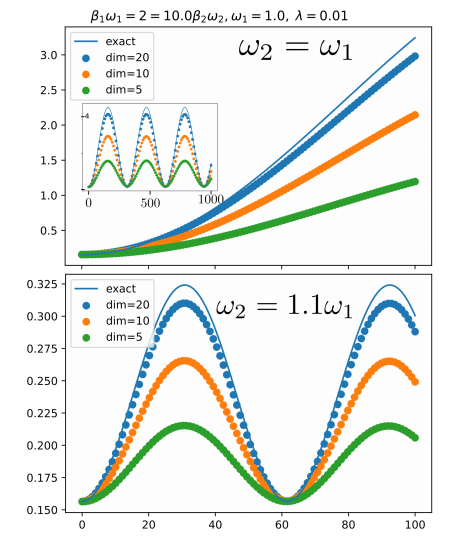
\includegraphics[scale=0.65]{figs/model3.1.3_fig1.png}
  \caption{Se muestra la evolución temporal del valor medio del operador número bosónico  ${\bf n}_1={\mathbf a}^\dagger{\mathbf a}$ obtenido del cálculo exacto \eqref{model3.1.3_ocupation_number} y los obtenidos mediante la simulación
  numérica del sistema truncado a dimensiones $5$, $10$ y $20$ para el caso resonante, (figura superior) y no resonante (figura inferior). }
  \label{model3.1.3_fig1}
\end{figure}

\section{Tratamiento aproximado: ecuaci\'on de Lindblad}\label{sec3_3TratamientoApproximado}

Una estrategia usual para estimar la evolución del estado reducido de un subsistema sin considerar explícitamente el estado de su entorno es mediante el uso de ecuaciones maestras. La ecuación de Lindblad provee entonces una aproximación a la dinámica local asumiendo ciertas hipótesis sobre la dinámica del entorno, que garantizan que el sistema sigue una dinámica completamente positiva. En el presente caso, donde el sistema está compuesto por sólo dos modos bosónicos, dichas condiciones están lejos de cumplirse.
Siguiendo los pasos detallados en \cite{HeinzPetruccione}, podemos construir una ecuación de Lindblad para el presente sistema como

 \begin{equation}
\frac{d\rho_A}{dt}=\frac{[{\bf H}_A-\Im(C) {\mathbf a}^\dagger {\mathbf a},\rho_A]}{{\bf i}\hbar } +  \Re(C)  \bigg[
  \langle {\mathbf b}^\dagger{\mathbf b}\rangle
\bigg({\mathbf a} \rho_A{\mathbf a}^\dagger - \frac{\{{\mathbf a}^\dagger{\mathbf a},\rho_A\}}{2}\bigg)
+\langle {\mathbf b}{\mathbf b}^\dagger\rangle
\bigg({\mathbf a}^\dagger \rho_A{\mathbf a} - \frac{\{{\mathbf a}{\mathbf a}^\dagger,\rho_A\}}{2}\bigg)
\bigg]\label{eq:lindbladbosA}
\end{equation}

con $\mathcal{C}=\lambda \int_{0}^{\infty} e^{{\bf i} (\omega_A-\omega_B)s}ds$. Naturalmente, esta integral no converge. Sin embargo, podemos regularizar esta cantidad introduciendo un tiempo de correlación $\tau$, y remplazando ${\cal C}$ por
$${\cal C}_\tau=\lambda\int_{0}^{\infty} e^{({\bf i} (\omega_A-\omega_B)-1/\tau) s}ds=\lambda\tau\frac{1+{\bf i}(\omega_A-\omega_B)\tau}{1+(\omega_A-\omega_B)^2\tau^2}$$
Podemos entender a $\tau$ como una escala de tiempo en la que el entorno pierde sus correlaciones, bien porque está acoplado a un sistema externo, bien porque lo observamos.

Notamos que como esta ecuación de Lindblad fue derivada de una dinámica gaussiana cerrada, y la traza de una matriz densidad gaussiana es gaussiana, las soluciones que corresponden a estados iniciales gaussianos evolucionan a estados gaussianos. Además, vemos que si inicialmente el estado era diagonal en la base de número de ocupación, lo será para todo tiempo posterior. Luego, si inicialmente el estado del sistema era de la forma

$$
\rho_A(0)=\frac{e^{-\beta(0){\mathbf a}^\dagger {\mathbf a}}}{{\Tr}e^{-\beta(0){\mathbf a}^\dagger {\mathbf a}}},
$$

para cualquier momento posterior tendremos

$$
\rho_A(t)=\frac{e^{-\beta(t){\mathbf a}^\dagger {\mathbf a}}}{{\Tr}e^{-\beta(t){\mathbf a}^\dagger {\mathbf a}}},
$$

que queda completamente determinado por el correspondiente valor medio del número de ocupación ${\bf n}_A(t)=\langle{\mathbf a}^\dagger{\mathbf a}\rangle_t$.

Podemos entonces resolver la evolución para esa familia de condiciones iniciales construyendo una ecuación para ${\bf n}_A(t)$. Para eso, multiplicando por derecha la Ec. \ref{eq:lindbladbosA} con $\frac{1}{\Re(C)}{\mathbf a}^\dagger{\mathbf a}$ y aplicando la operación de traza, obtenemos luego de algunas manipulaciones 

\begin{equation}
  \label{eq:lindbladoneside}
\frac{1}{\Re(C)}\frac{d {\bf n}}{dt}= {\bf n}_B-{\bf n}_A,
\end{equation}

cuya solución es de la forma

$$
{\bf n}_{A}(t)={\bf n}_{B}(0)+({\bf n}_{A}(0)-{\bf n}_{B})e^{-\Re(C)t },
$$

Si por otro lado, admitimos que como ambos sistemas son equivalentes, $n_B$ debería tener una dinámica idéntica a la de $n_A$, de manera que el número de partículas total se conserve, podemos generalizar \ref{eq:lindbladoneside} al par de ecuaciones acopladas de primer orden Lifshitz-continuas

% el n(t) ya no se conserva 

\begin{eqnarray}
  \label{eq:lindbladtwoside}
  \frac{1}{\Re(C)}\frac{d {\bf n}_A}{dt}&=& {\bf n}_B-{\bf n}_A\\
  \frac{1}{\Re(C)}\frac{d {\bf n}_B}{dt}&=& {\bf n}_A-{\bf n}_B,
\end{eqnarray}

cuya solución es de la forma

$$
{\bf n}_A(t)=\frac{{\bf n}_{A}(0)-{\bf n}_B(0)}{2}e^{-2 \Re(C) t} + \frac{{\bf n}_{A}(0)+{\bf n}_B(0)}{2}=\frac{{\bf n}_{A}(0)+{\bf n}_B(0)}{2}-{\bf n}_{B}(t).
$$

En la figura \ref{fig:model3.1.3_lindblad-vs-exact} se muestra el comportamiento del número de ocupación bosónico del primer sistema ${\bf n}_1 $ \textit{vs. t} para distintos tiempos y valores de regularización, tanto para el caso resonante como no resonante. 

Luego, la discrepancia de resultados - sobretodo para el caso no resonante - implica que, desde un enfoque de sistemas dinámicos, el sistema no cumple la ecuación de Lindblad localmente, o lo hace para tiempo nulo. En todo caso, vemos que el sistema relaja luego de un tiempo - que depende del parámetro de regularización $\tau$ - a un estado en que el número de partículas de ambos sistemas es el mismo, comportamiento bastante diferente al que obtuvimos de la evolución exacta. Notamos sin embargo que para tiempos grandes, en el caso resonante, la ocupación predicha por Lindblad converge al promedio temporal de la ocupación predicha por el modelo exacto. 

\begin{figure}
  \centering
  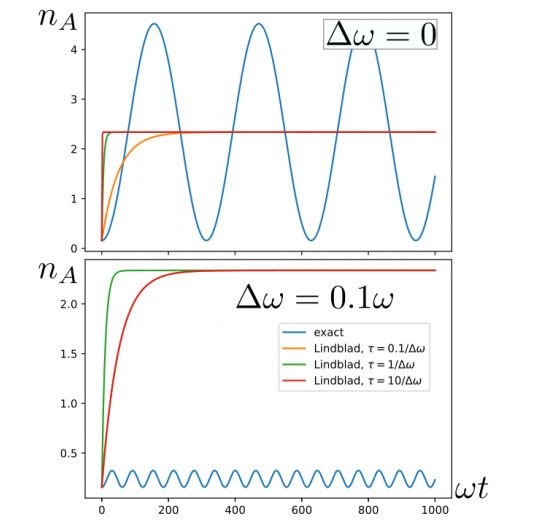
\includegraphics[scale = 0.65]{figs/model3.1.3_lindblad-vs-exact.png}
  \caption{Número de ocupación exacto y estimado al resolver la ecuación de Lindblad para diferentes valores de la regularización. Arriba: caso resonante. Abajo: $\Delta \omega/\omega=0.1$. En ambos casos se consider\'o el caso $\lambda=0.01 \hbar \omega$.}
  \label{fig:model3.1.3_lindblad-vs-exact}
\end{figure}

%\subsubsection{Resultados analíticos para estados gaussianos de un modo}
\begin{Omitir}

\begin{equation}
\rho=\frac{e^{-\beta {\bf n}}}{{\Tr}e^{-\beta {\bf n}}}
\end{equation}
$$
Z={\Tr}{e^{-\beta {\bf n}}} = \frac{1}{1-e^{-\beta}}
$$

$$
n= \langle n\rangle ={\Tr}{\bf n}\rho = \frac{1}{e^{\beta}-1}
$$
$$
\beta=\ln(\frac{n+1}{n})
$$
$$
Z=n+1
$$
$$
S(\rho)=-{\Tr}\rho \ln \rho = \beta n +\ln(n+1)
$$

$$
S(\rho_1||\rho_2)=n_1 \ln(\frac{n_1}{n_2})+ (n_1+1)\ln(\frac{1+n_2}{1+n_1})
$$
\end{Omitir}

Finalmente, a modo de conclusión del presente capítulo, se incluye en el apéndice \ref{ApendixA} un tratamiento perturbativo a la dinámica abierta del sistema de dos bosones como también así también la de un sistema bosónico genérico en la que se buscan estudiar algunas propiedades de dichos sistemas.
\clearpage

\chapter{Max-Ent y din\'amica aproximada}
\label{chap4_allmaxent}

\section*{Validez de la aproximaci\'on Markoviana.}

En el capítulo anterior, específicamente en la sección \ref{sec3_3TratamientoApproximado}, se estudió la evolución
del estado reducido de un modo bosónico, en un sistema que inicialmente se encontraba en un estado gaussiano descorrelacionado 
cuyas caracter\'isticas no son conocidas, mediante el uso de la ecuaci\'on maestra de Lindblad 
caracterizado por los t\'erminos de colapso que este induce. 
Al haber hecho uso de la ecuación de Lindblad, implícitamente se asumió la Markovianidad del sistema. Luego de completar los cálculos se encontró que la ecuación de Lindblad no devuelve resultados fidedignos con la dinámica exacta puesto que, acorde al formalismo de Lindblad, el sistema relaja a un estado en el que el número de partículas de ambos sistemas es el mismo, lo cual no se condice con los resultados de la evolución exacta. Esto se debe a que la aproximación Markoviana implementada no tiene en cuenta las correlaciones generadas durante la evolución. 

Una forma de subsanar esta discrepancia es resolviendo la dinámica exactamente. Sin embargo, en muchos casos la resolución de las ecuaciones diferenciales es un problema muy costoso y complejo, por lo que hemos de hacer uso de otras aproximaciones no-markovianas. 
En este trabajo, trataremos los distintos sistemas mediante un formalismo de \textbf{Gaussianización} basado en la propiedad \textbf{Max-Ent}.

\section*{Gaussianizaci\'on como aplicaci\'on del principio Max-Ent}

Anteriormente se ha estudiado la aplicabilidad de dinámicas Gaussianas a sistemas bosónicos, encontrando que este es un formalismo útil para la descripción de dichos sistemas. La ventaja de este formalismo radica en la reducción de la complejidad de un problema $\mathcal{O}(2^n)$ en un problema donde se han de especificar únicamente ciertos parámetros del estado Gaussiano, un problema $\mathcal{O}(n^2)$. Sin embargo este formalismo tiene sus límites y se vuelve inaplicable en el régimen de altas temperaturas y correlaciones grandes puesto que los mapeos bosónicos implementados dejan de ser fidedignos al problema original, requieriendo entonces de implementar un nuevo formalismo para aproximar al estado del sistema estudiado.

Este nuevo formalismo que usaremos para aproximar al estado exacto de un sistema evolucionado se basa en que los estados Gaussianos son estados Max-Ent con correlaciones de pares, por lo que siempre será posible aproximar al estado del sistema sin recurrir explícitamente al mapeo bosónico, trabajando directamente sobre dichos parámetros.

\clearpage

\section{Formalismo Max-Ent}
\label{ch_Max-Ent1}

Para entender este principio, supongamos que queremos determinar el estado inicial de un cierto sistema físico. Para hacerlo, debemos conocer, por medio de medidas sobre muchas copias del sistema, los valores medios de un conjunto completo de observables independientes. Llamamos al procedimiento de reconstruir el estado a partir de esos valores medios una \textbf{reconstrucción tomográfica} \cite{Nielsen.00} del estado.

Por ejemplo para un sistema de espín 1/2 esto se reduce a medir los valores medios de sus componentes ortogonales respecto a algún sistema de coordenadas. Por otro lado para un sistema de dos qubits, la caracterización de dicho sistema requerirá de la determinación experimental de 15 parámetros reales  \cite{Nielsen.00, mQC_Brylinski}.
Esto se puede realizar mediante una elección óptima de cinco observables que constituyen un conjunto completo de observables. De estos quince parámetros a determinar, seis se corresponden a observables locales y nueve a correlaciones de pares\footnote{Esto permite distinguir seis clases de estados localmente equivalentes. En este caso, la equivalencia local implica que existe una diferencia topológica y geométrica entre estos estados y, no una diferencia fundamentalmente física.}.
 
En general, al aumentar la dimensión del sistema, el número de observables necesarios para determinar el estado del sistema crece exponencialmente.
Por otro lado, en sistemas compuestos, s\'olo se tiene acceso a un n\'umero mucho m\'as limitado de observables, 
generalmente limitados a valores medios locales y correlaciones de pares, lo que no es suficiente para una reconstrucción tomográfica completa.
De esta manera, existirán muchos estados posibles \emph{compatibles} con los observables determinados. Podemos preguntarnos entonces cuál es el estado menos \emph{sesgado} que podemos asumir para el sistema. 

Un criterio para tal estado lo da el principio Max-Ent: de todos los estados, este principio establece que el estado menos 'sesgado' es aquel  estado,  compatible con los valores medios determinados, y cuya entropía de von Neumann es máxima,

\begin{equation*}
\rho\approx \rho_{ME} = \arg\max_{{ \Tr}\sigma {\bf O}_i =\langle  O_i\rangle} S(\sigma).
\end{equation*}

Podemos entender este criterio de la siguiente manera. Supongamos que tenemos diferentes estados candidatos $\sigma_i$ que cumplen la condición sobre los valores medios conocidos. Entonces,

\begin{equation*}
\sigma =\sum_i p_i \sigma_i,
\end{equation*}

donde $\{\{p_i\}_{i=1} \in \mathds{R}_{[0, 1]} \textnormal{ | }\sum_i p_i=1\}$, es otro estado que también cumple la misma condición sobre los valores medios, pero asume como conocida menos información: a priori, cualquiera de los $\sigma_i$ es igual de aceptable. Por otro lado, por la convexidad de la entropía de von Neumann,

\begin{equation*}
S(\sigma)\geq \sum_i p_i S(\sigma_i),
\end{equation*}
de lo que se sigue que este mejor candidato tendrá una mayor entropía. Esto es consistente con la idea de que es un estado que asume menos información conocida. 

Si pensamos a la condición sobre los valores medios como una restricción lineal, podemos utilizar el teorema de los multiplicadores de Lagrange para encontrar la forma del estado. Para eso, observamos que el problema de maximizar la entropía para ciertos valores medios determinados puede reformularse como la maximización de un problema sin restricciones:

\begin{eqnarray}
\rho_{ME} &=& \arg\max_{\sigma} {\bf F}[\sigma]\,;\mbox{ con }\\
{\bf F}[\sigma]&=&S(\sigma)+\sum_i \lambda_i ({\Tr}\sigma{ \bf O}_i-\langle {\bf O}_i\rangle)
\label{max-ent_def1}
\end{eqnarray}
para una cierta elección de los multiplicadores $\lambda_i$. Proponiendo $\sigma=\rho+\delta \sigma$ tendremos que

\begin{equation*}
{\bf F}[\sigma]=S(\rho)+
{\Tr}\delta \sigma (\lambda_i {\bf O}_i-\ln \rho)
{\cal O}^2(\delta \sigma),
\end{equation*}
\noindent por lo que \begin{equation}
\rho_{ME}=\frac{e^{-\sum_i \lambda_i {\bf O}_i}}{{Tr}e^{-\sum_i \lambda_i {\bf O}_i}}.
\label{eq:estadogibbsgeneralizado}
\end{equation}
para ciertos valores de los multiplicadores $\lambda_i$. En particular, si el observable a fijar es la energía del sistema, el operador densidad correspondiente tomará la forma de un \textbf{estado de Gibbs} \cite{PATHRIA2011115}. Esto motiva a llamar a los estados de la forma \ref{eq:estadogibbsgeneralizado} la familia de \textbf{estados de Gibbs generalizados} ó  \textbf{estados Max-Ent} para los observables ${\bf O}_i$:

\begin{equation*}
\mathfrak{G}_{\{{\bf O}_i\}}:=\{\rho \in \mathcal{C}(\mathds{H})\textnormal{ | } \exists \{\lambda_i\}_{i=1} \in \mathds{R} \land \exists \{{\bf O}_i\}_{i=1}  \textnormal{ tal que }  \rho=\frac{e^{-\sum_i \lambda_i {\bf O}_i}}{\Tr e^{-\sum_i \lambda_i {\bf O}_i}}\},
\label{Gibbs_state}
\end{equation*}

Esto nos permite obtener una caracterización alternativa para los estados Max-Ent: Si $\rho_{0}$ es el estado exacto del sistema, $\rho_{ME}$ es aquel estado de la familia $\mathfrak{G}_{\{{\bf O}_i\}}$ que \emph{minimiza}
la entropía relativa con $\rho_0$:

\begin{equation}
\rho_{ME}= {\arg}\min_{\sigma \in {\cal G}_{\{{\bf O}_i\}}}S(\rho_0||\sigma),
\end{equation}

\begin{Omitir}
la información de un sistema cuántico es deficiente y no es suficiente para caracterizar completamente un estado. En tal caso, existe más de una distribución de probabilidad que sea compatible con el sistema. Luego, el Principio Max-Ent formulado por Jaynes consiste en elegir aquella que maximice la entropía de von Neumann.

Supongamos que de dicho sistema solamente disponemos de un número limitado de resultados, los valores de expectación de algunos observables físicos $\lgg {\bf O}_1 \rgg_{obs}$, $\lgg {\bf O_2}_1 \rgg_{obs} \ldots, \lgg {\bf O}_k \rgg_{obs}$. Como no disponemos de suficiente información sobre el sistema, no podremos realizar un análisis tomográfico y determinar analíticamente el estado del sistema. En tal caso, existirán múltiples operadores densidad  $\rho_1, \rho_2, \ldots$ compatibles con los vínculos del sistema tales que 

\begin{align}
\left\{ \begin{array}{lcc}
          \lgg {\bf O}_1 \rgg_{\rho_j} = \lgg {\bf O}_1 \rgg_{obs}  \\
          \vdots     \\ 
          \lgg {\bf O}_k \rgg_{\rho_j} = \lgg {\bf O}_k\rgg_{obs}  \\ 
             \end{array}
\right.
\label{me_1}
\end{align}
con $j=1,2,\ldots,k$. Luego, una posible definición para el estado Max-Ent es 
\begin{equation}
   \rho_{ME} = \arg\max_{\sigma | \lgg {\bf O}_j \rgg_{\rho_j} S(\sigma)= \lgg {\bf O}_j \rgg_{obs}}. 
    \label{max-ent_def1}
\end{equation}
donde $\rho_{ME}$ denota al estado Max-Ent, $S(\sigma)$ denota a la entropía de von Neumann del estado $\sigma$ sujeto a las condiciones \eqref{me_1}  y donde nuevamente $j=1,2,\ldots,k$.

Por otro lado definimos el set de \textbf{estados de Gibbs}, denotado por $\mathfrak{G}\{{\bf O}_i\}$,  como aquellos estados que pueden ser escritos como 
\begin{equation}
    \rho = \frac{\exp(-\alpha_i {\bf O}_i)}{\Tr \exp(-\alpha_i {\bf O}_i)}, 
    \label{Gibbs_state}
\end{equation}
\noindent donde $\alpha_i \in \mathds{R}^n$, donde la operación de $\Tr$ se ha de realizar sobre todos los estados del espacio de Hilbert compatibles con los vínculos del sistema 
\end{Omitir}
\begin{Omitir}
y donde $\mathbf{K}$ es una forma cuadrática escrita en términos de los operadores bosónicos $\mathbf{a}_i$ y $\mathbf{a}_i^{\dagger}$ que cumplen un álgebra cerrada de conmutadores a saber:
\begin{align}
    [\mathbf{a}_i,\mathbf{a}_j] & = [\mathbf{a}_i^{\dagger},\mathbf{a}_j^{\dagger}] =0;  &  [\mathbf{a}_i, \mathbf{a}_j^{\dagger}] = \delta_{ij}.
    \label{Bosonic algebra}
\end{align}

Esta álgebra genera un espacio de Fock bosónico, que surge como el espacio de representación sobre el cual actúa el álgebra \eqref{Bosonic algebra}. 

Por otro lado, existe una definición alternativa y equivalente para el estado Max-Ent. Acorde a esta definición, el estado Max-Ent es aquel que cumple la siguiente condición 

\begin{equation}
\tilde{\rho} = \min_{\atop{\sigma \in \mathfrak{G}\{{\bf O}_i\}}} S(\rho || \sigma) = \rho_{ME} \bigg|_{\lgg {\bf O}_i\rgg = \lgg {\bf O}_i\rgg_{\rho}},   
\label{max-ent_def2}
\end{equation}

donde $S(\rho||\sigma) = - \Tr \rho (\log \sigma - \log \rho)$, la entropía relativa entre dichos estados $\rho$ y $\sigma$. Resulta que el estado $\rho_{ME}$ definido por \eqref{max-ent_def1} y \eqref{max-ent_def2} puede ser escrito como un estado de Gibbs \eqref{Gibbs_state}. Un caso particular de los estados Max-Ent son los Estados Gaussianos, ya introducidos anteriormente. 
Son estados simultáneamente Max-Ent y de Gibbs. \\
\end{Omitir}


Un conjunto de estados $\mathfrak{g}_{\{{\bf O}_i\}}$ representa entonces una subvariedad (Riemanniana) del conjunto de los operadores densidad del sistema $\mathcal{C}(\mathds{H})$. Sin embargo, y a diferencia de 
(excepto para casos límites triviales), $\mathfrak{g}_{\{{\bf O}_i\}}$ no será un conjunto convexo: la mezcla estadística de dos estados en $\rho, \sigma \in \mathfrak{g}_{\{{\bf O}_i\}}$ en general no pertenece a dicho espacio, $p \rho + (1-p) \sigma \notin\mathfrak{g}_{\{{\bf O}_i\}}$. Por ejemplo, si ${\bf s}_z=|1\rangle\langle 1|-|-1\rangle\langle -1|$ representa la componente $z$ del espín de una partícula de espín $1$,
$\rho_{\pm}=e^{\mp \beta{\bf s}_z}/{\Tr}e^{\mp \beta{\bf s}_z} \in  \mathfrak{g}_{\{s_z\}}$,  pero
$$
\rho=\frac{e^{- \beta{\bf s}_z}+e^{\beta{\mathbf s}_z}}{2 \mathrm{Tr}e^{- \beta{\mathbf s}_z}} \not\in 
\mathfrak{g}_{\{s_z\}}
$$

\section{Estados Max-Ent de uno y dos cuerpos}

Habiendo definido en general la familia de estados max-ent $\mathfrak{G}_{\{O_i\}}$, y a los efectos de la discusión siguiente, vamos a introducir dos casos particularmente relevantes: el de las familias de estados Max-Ent de uno y dos cuerpos. Para esto, vamos a considerar un sistema cuántico compuesto, de manera que su álgebra de observables sea generada por las álgebras de observables en cada subsistema que lo conforma:
$$
{\cal A}_S = \overline{\bigcup_i {\cal A}_i}
$$
con ${\cal A}_i=\overline{\{{\bf o}_{1,i},{\bf o}_{2,i},\ldots\}}$ el álgebra de observables asociada al sub-sistema $i-$ésimo, de manera que cualquer operador ${\bf Q}$ en ${\cal A}_i$ sea una combinación lineal de productos de los operadores ${\bf o}_{1,i}$.

Diremos entonces que un operador ${\bf O}_1$ es un \emph{operador de un cuerpo} si puede expresarse como una combinación lineal de los operadores ${\bf o}_{1,i},{\bf o}_{2,i},\ldots$ que definen una o varias de las subálgebras locales. En general, diremos que un operador es de $n-$cuerpos si puede expresarse como combinación lineal de productos de hasta $n$ operadores de $1$ cuerpo. De esta manera, ${\bf 1}$ sería un operador de $0-$cuerpos, la proyección $z$ del momento angular total en un sistema de espines ${\bf S}_z=\sum_i {\bf s}_{z,i}$ sería un operador de $1-$cuerpo, y el cuadrado del momento angular total ${\bf S}^2={\bf S}_x^2+{\bf S}_z^2+{\bf S}_z^2$, un operador de dos cuerpos \footnote{Notemos que con esta definición, un operador de un cuerpo será también un operador de dos cuerpos}.

Conviene entonces definir la \emph{variedad max-ent de 1-cuerpo} (\emph{2-cuerpos})  $S_{ME, 1}=\mathfrak{g}_{1-cuerpo}$ ($S_{ME, 2}=\mathfrak{g}_{2-cuerpo}$), como el conjunto de estados que maximizan la entropía luego de fijar los valores medios para todos los operadores de 1 cuerpo (2 cuerpos)\footnote{En general, podemos definir $S_{ME, n}$ como el conjunto de estados max-ent con valores medios definidos para todos los operadores de hasta $n$ cuerpos.}.

Por lo tanto, $S_{ME, 1}$ es un conjunto de estados producto (no correlacionados), que es a la vez una subvariedad de $S_{ME, 2}$.
$S_{ME, 2}$ está formada entonces por un conjunto de estados max-ent para los que están fijadas solamente las correlaciones de pares. 



\begin{Omitir}
Sea nuevamente el \textbf{espacio de estados}, denotado por $\mathcal{C}(\mathds{H})$, el conjunto de todos los estados densidad compatibles con los vínculos de un sistema cuántico el cual es un conjunto convexo que tiene la estructura topológica de una variedad Riemanniana, cuya métrica está dada por aquella que rige el producto escalar de Hilbert-Schmidt \eqref{HS scalar prod} \cite{Nielsen.00, NakaharaM}. Dentro de dicha variedad, disponemos de otras dos subvariedades relevantes a este trabajo, a saber: aquella asociada a los \textbf{estados Max-Ent de un cuerpo}, denotado por $\mathcal{S}_{ME,1}$, y aquella asociada a los \textbf{estados Max-Ent de dos cuerpos}, denotado por $\mathcal{S}_{ME,2}$. 

Notamos que estas dos variedades no son convexas puesto que la  mezcla estadística de dos estados Max-Ent cualesquiera en $\mathcal{S}_{ME,1}$ ($\mathcal{S}_{ME,2}$) en general no pertenece a $\mathcal{S}_{ME,1}$ ($\mathcal{S}_{ME,2}$). Por ejemplo, $\rho_{\pm}=e^{\mp \beta{\bf s}_x}/{\Tr}e^{\mp \beta{\bf s}_x} \in \mathcal{S}_{ME,1}$,  pero

$$
\rho=\frac{e^{- \beta{\bf s}_x}+e^{\beta{\mathbf s}_x}}{2 \mathrm{Tr}e^{- \beta{\mathbf s}_x}} \not\in 
\mathcal{S}_{ME,1}
$$

Adicionalmente, notamos que la variedad $\mathcal{S}_{ME,1}$ es, a su vez, una subvariedad de $\mathcal{S}_{ME,2}$ en el cual los estados no tienen correlaciones de pares. \\
\end{Omitir}

\section{Estados Max-Ent y gaussianizaci\'on}

En esta sección explicaremos como se puede aplicar el formalismo de gaussianización y el formalismo Max-Ent en el modelado de la dinámica de sistemas cuánticos. En la figura \ref{aprox-ME1_page-0001.jpg}, mostramos la aproximación Max-Ent para un sistema cuántico a un tiempo fijo. Disponemos de un estado $\rho$ en el espacio de estados, luego, mediante un proceso de optimización de los parámetros de cada clase de estados, obtendremos un estado $\sigma_1 \in \mathcal{S}_{ME,1}$ y un estado $\sigma_2 \in \mathcal{S}_{ME,2}$, que aproximarán al estado exacto del sistema. Como el estado Max-Ent de dos cuerpos incluye correlaciones de dos cuerpos, este aproximará mejor al estado real del sistema comparado al estado Max-Ent de un cuerpo, debido a la mayor cantidad de parámetros disponibles a optimizar. Esta noción de distinguibilidad entre operadores se obtiene, en este caso, mediante la entropía relativa entre dos estados dada por \ref{relative entropy} para cualquier par de estados $\rho$ y $\sigma$. 
%\footnote{Cabe destacar que tanto la entropía relativa, dada por \eqref{relative entropy}, como la fidelidad, dada por \eqref{fidelity}, no son métricas; sino simplemente medidas de distinguibilidad. La entropía relativa no es una métrica puesto que no es simétrica y la fidelidad tampoco es una métrica al no cumplir con la desigualdad triangular. En particular la entropía relativa se anula cuando los estados son idénticos y decrece cuando los estados son menos distinguibles. Una métrica bien definida está dada por el arcocoseno de la fidelidad, la métrica de Bures-Wooters \eqref{Bures-Wooters} }

\begin{figure}
    \centering
    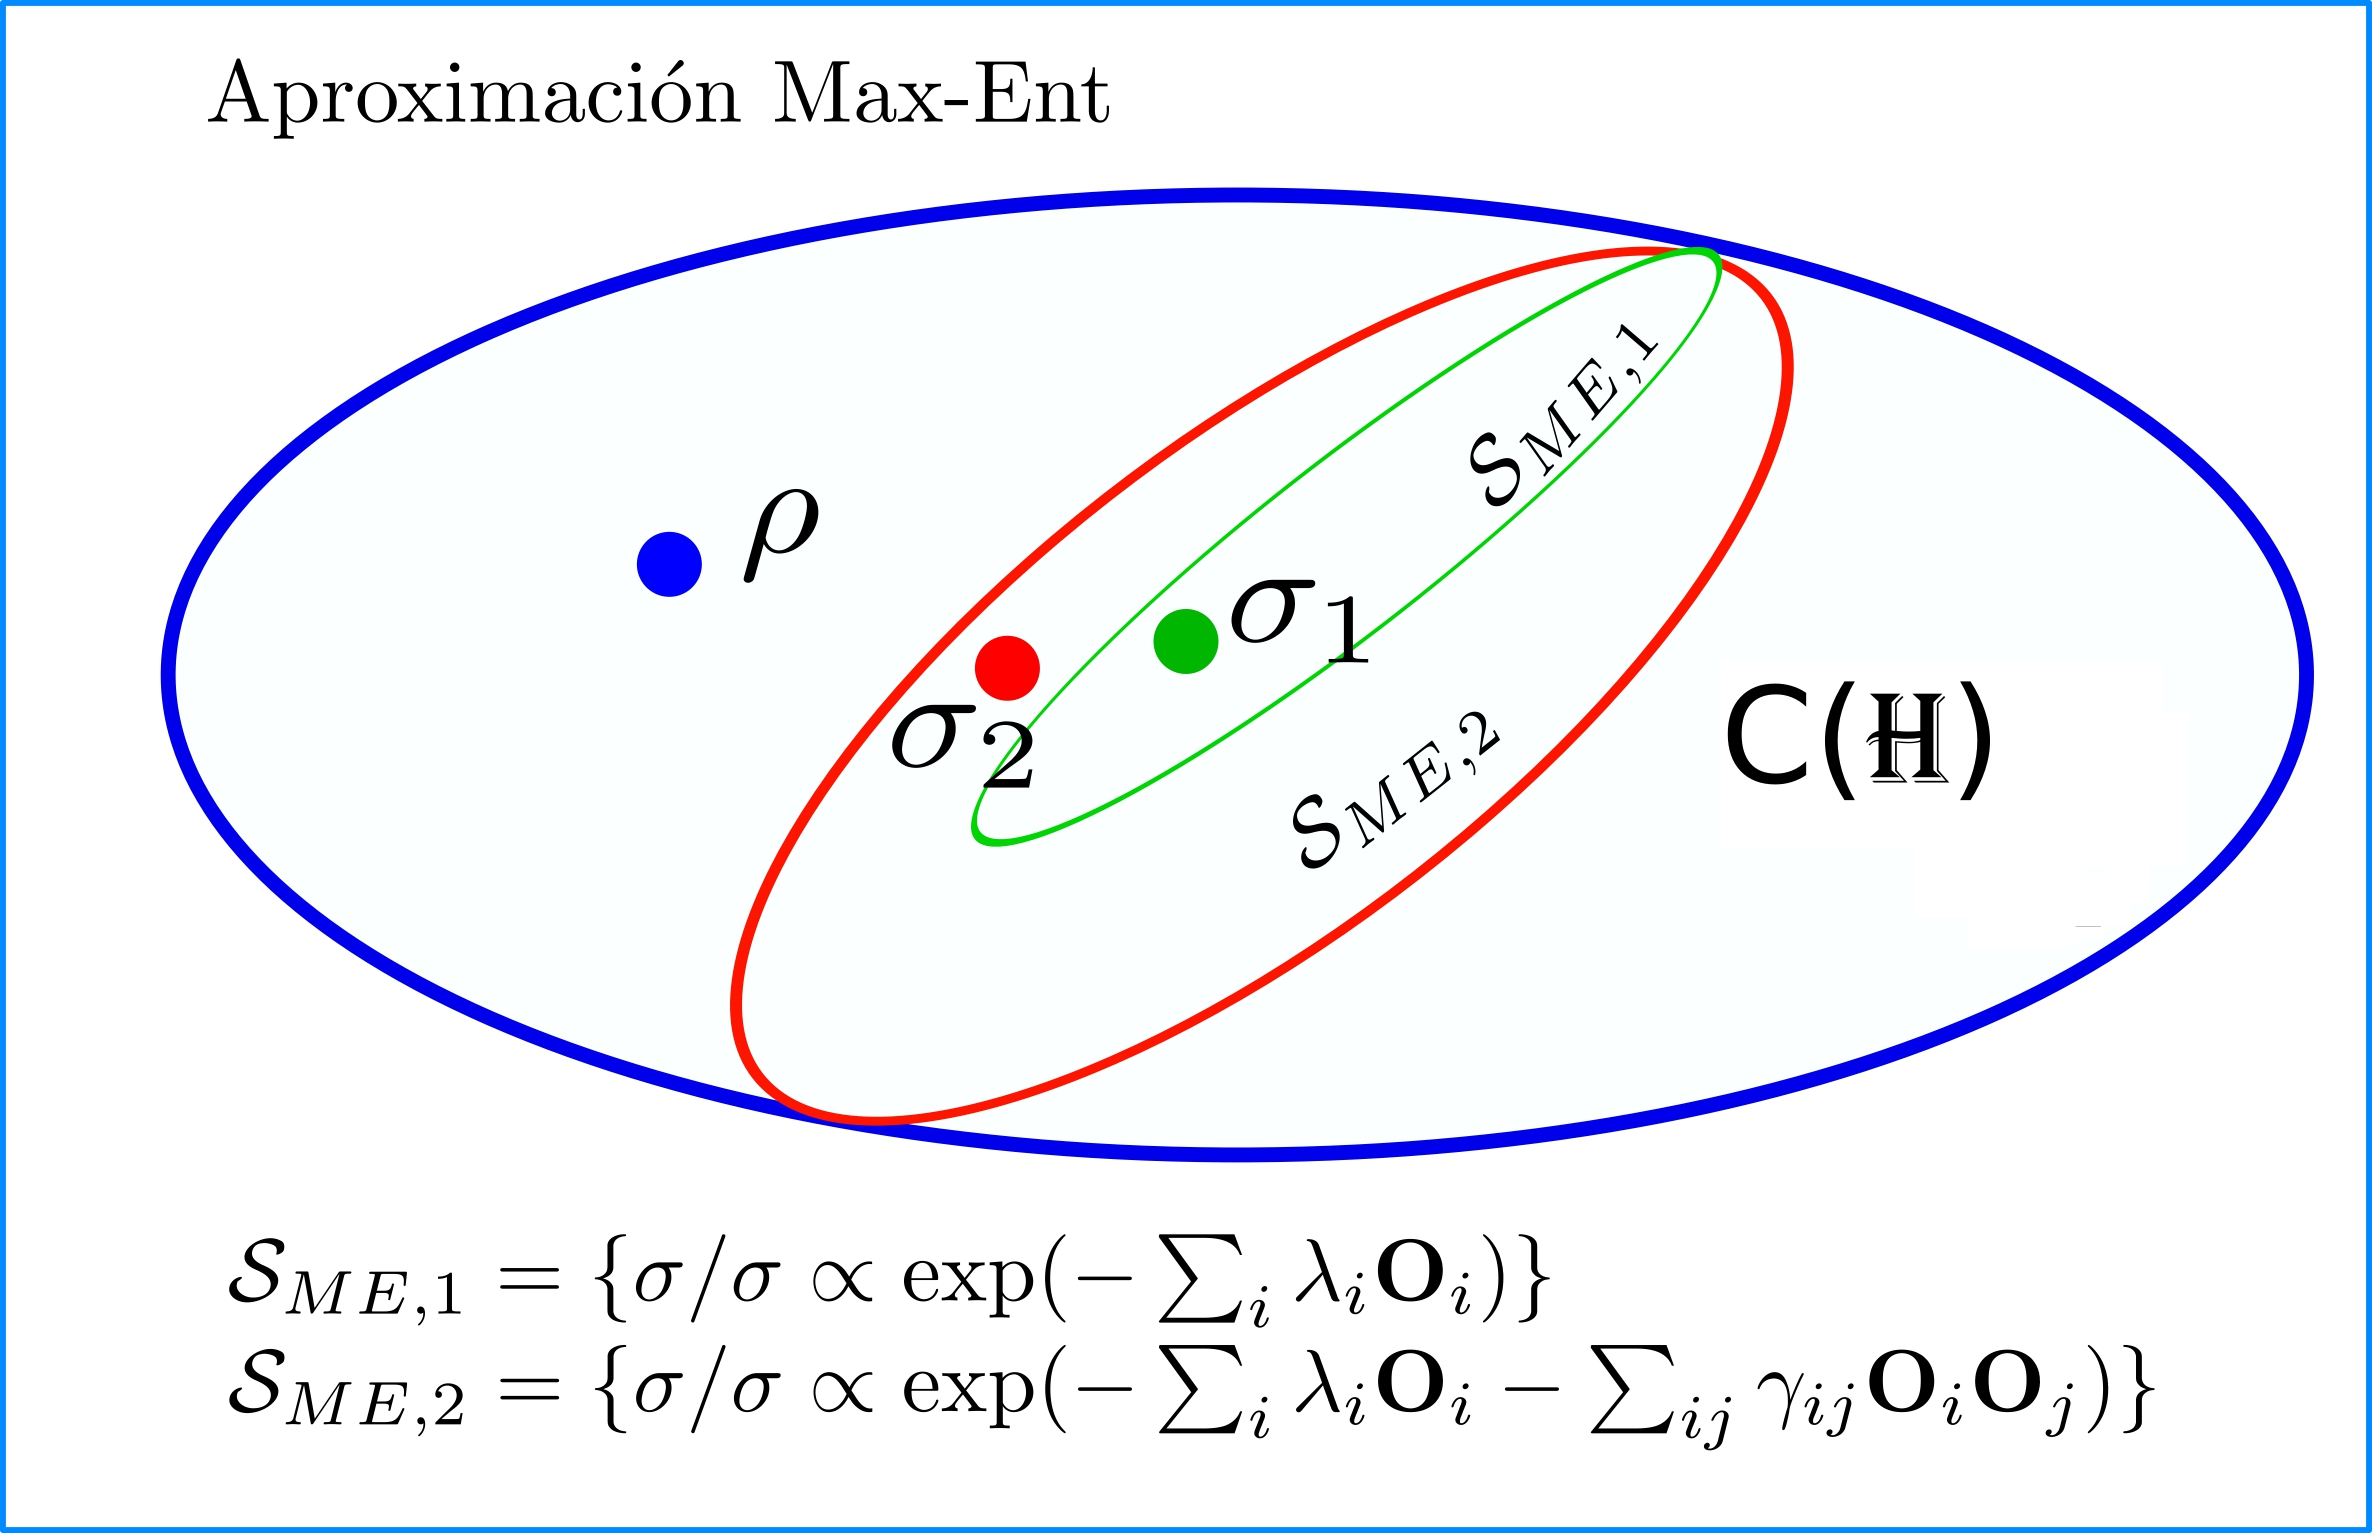
\includegraphics[scale=0.2]{figs/aprox-ME1_page-0001.jpg}
    \caption{En el presente diagrama, mostramos la variedad de estados densidad $\mathcal{S}$. Dentro de dicha variedad encontramos otras dos variedades: una asociada a estados Max-Ent de un cuerpo $\mathcal{S}_{ME,1}$ (en \textcolor{green}{verde}) y otra variedad de Max-Ent de dos cuerpos $\mathcal{S}_{ME,2}$ (en \textcolor{red}{rojo}), la cual incluye a la anterior. Mediante un proceso de optimización de los parámetros obtendremos los mejores estados, aquellos que más aproximan al estado del sistema, manteniéndose dentro de su variedad: el estado $\sigma_1$ dentro de la variedad $\mathcal{S}_{ME,1}$ y $\sigma_2$ dentro de la variedad $\mathcal{S}_{ME,2}$  }
    \label{aprox-ME1_page-0001.jpg}
\end{figure}

\begin{figure}
    \centering
    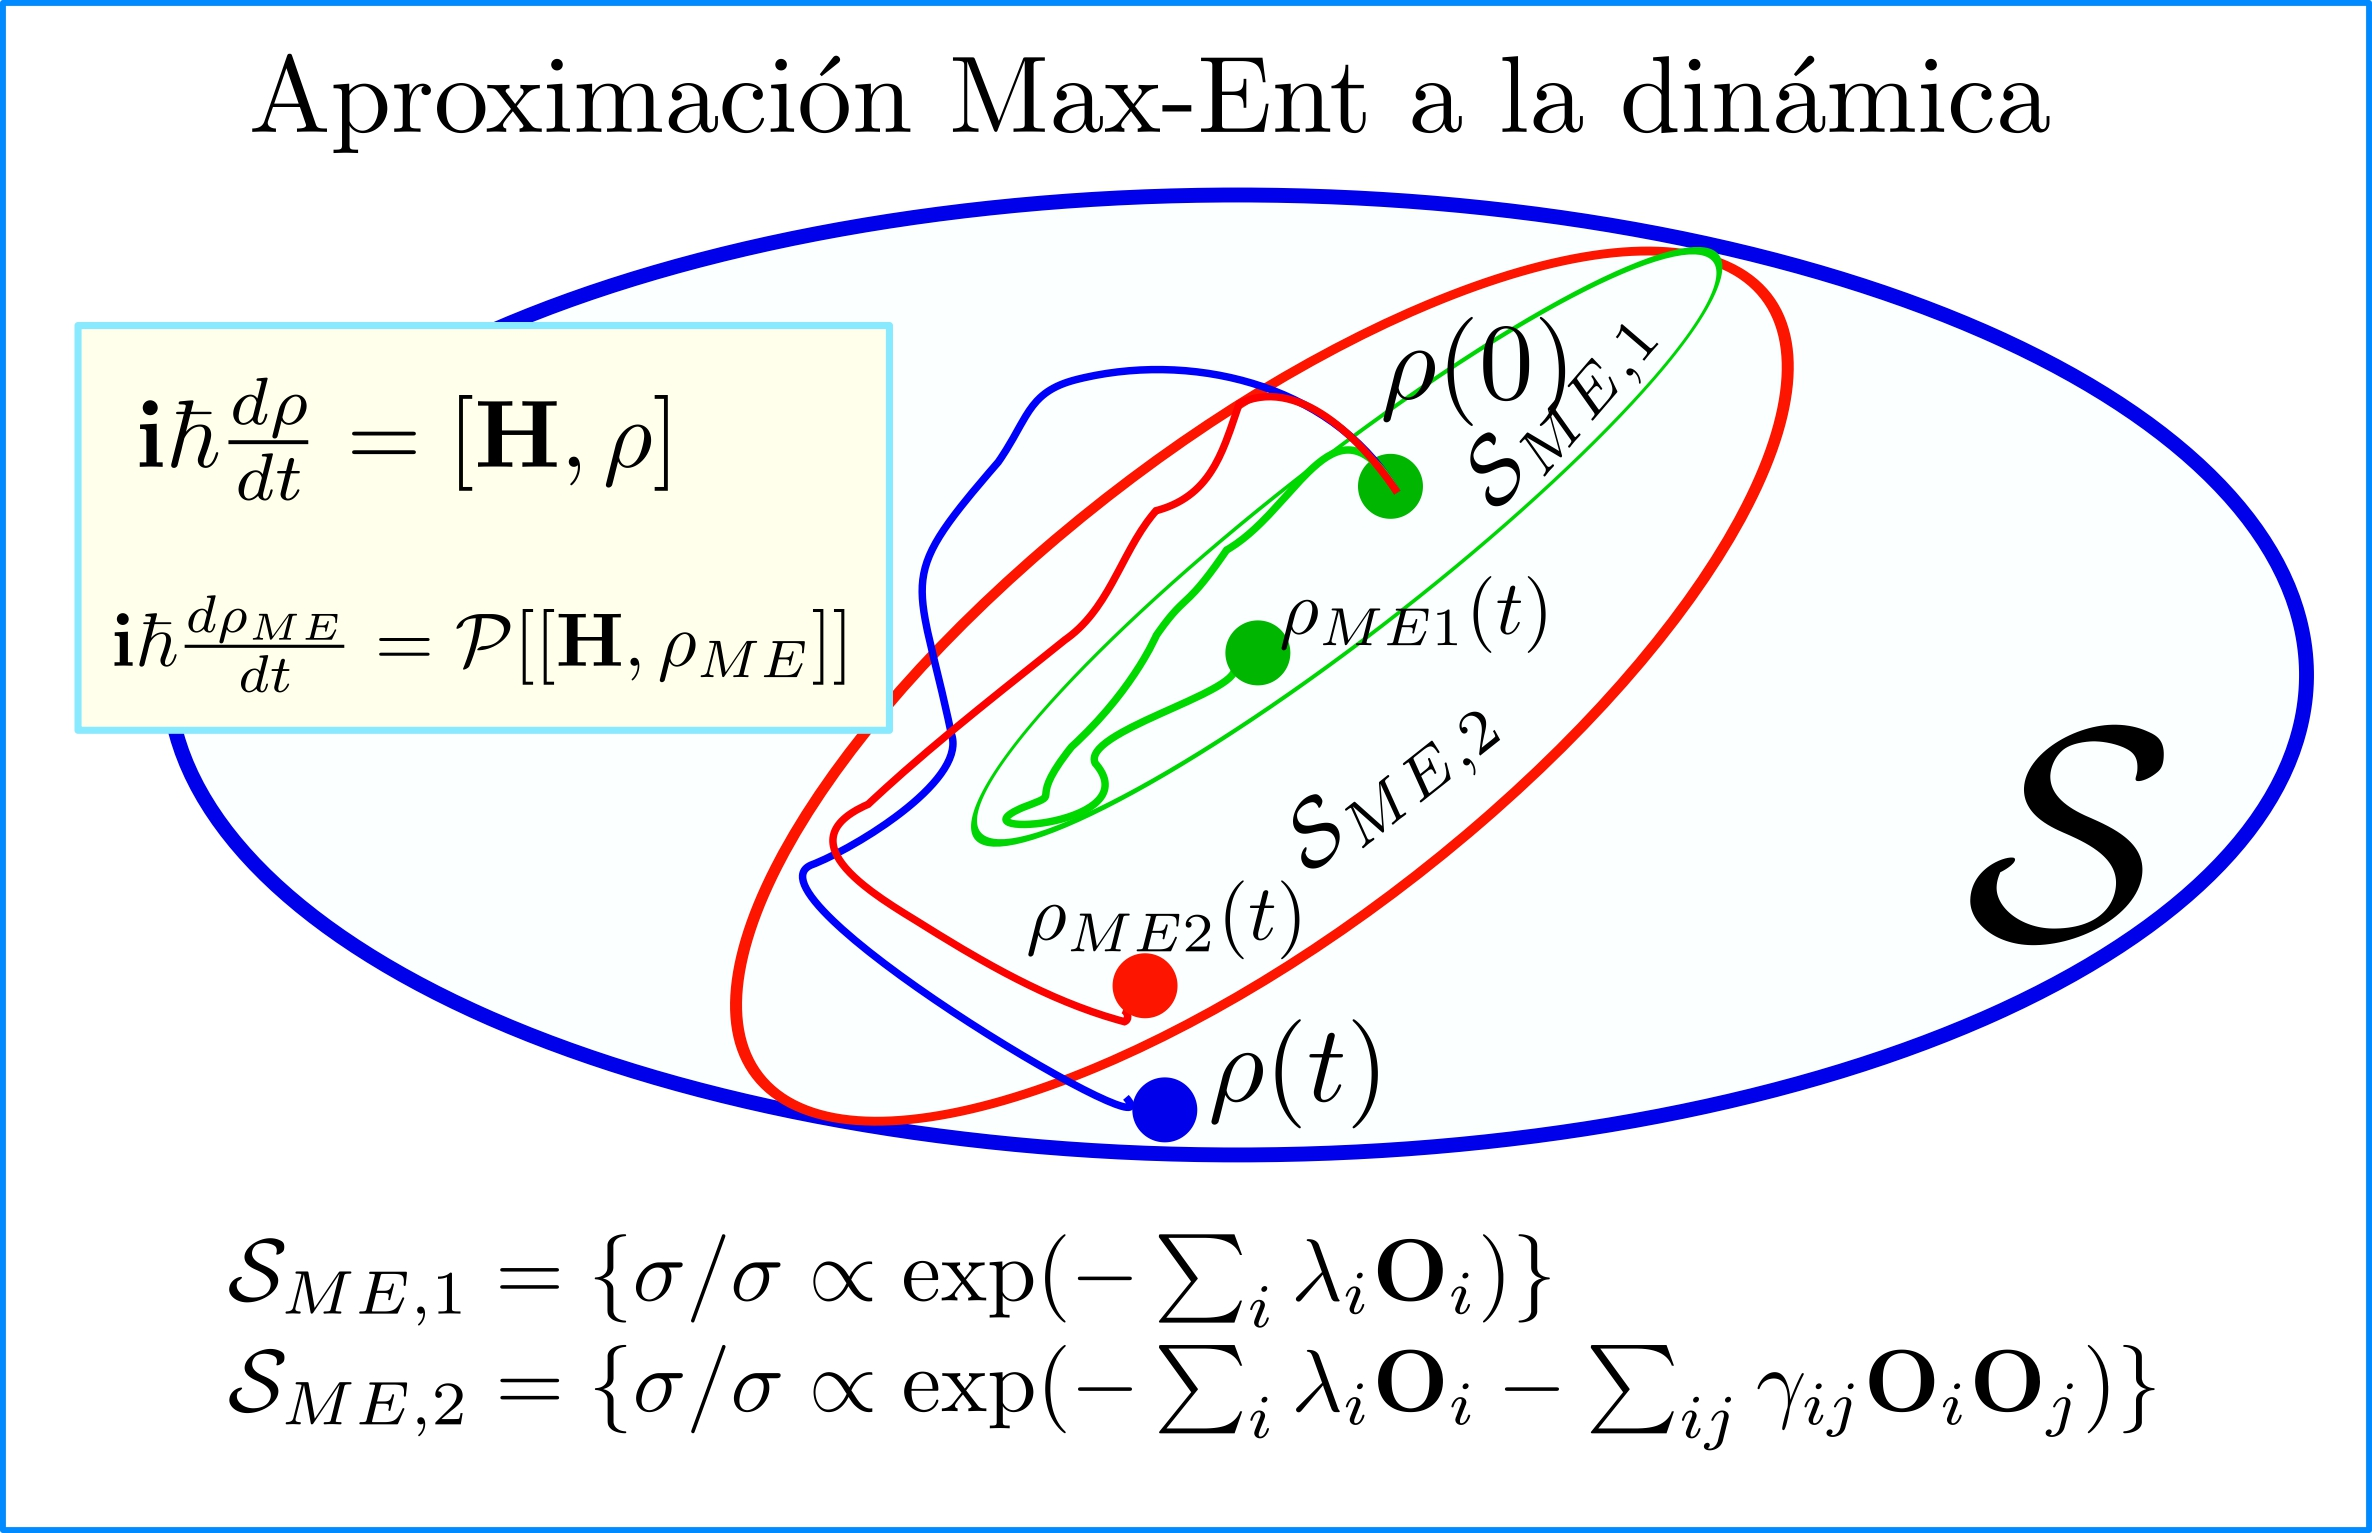
\includegraphics[scale=0.2]{figs/aprox-ME2_page-0001.jpg}
    \caption{En este diagrama mostramos la aplicación de las aproximaciones Max-Ent de uno y dos cuerpos para el estudio de la dinámica de un sistema cuántico. Nuevamente, desconocemos la forma explícita del estado, inicialmente descorrelacionado, del sistema, $\rho(t)$ denotado en azul, por lo que buscamos aproximarla con dinámicas restringidas Max-Ent de un cuerpo, $\sigma_1(t)$ en \textcolor{green}{verde}, y el estado Max-Ent de dos cuerpos  $\sigma_2(t)$ en \textcolor{red}{rojo}. En ambos casos, los estados $\sigma_1(t)$ y $\sigma_2(t)$ continuarán siendo estados Max-Ent de uno y dos cuerpos, respectivamente, para todo tiempo sin salirse de la variedad a la cual pertenecen. }
    \label{aprox-ME2_page-0001}
\end{figure}

%Por lo tanto haremos uso de las \textbf{dinámicas restringidas de Max-Ent de uno y dos cuerpos}, es decir dinámicas Max-Ent donde se fuerza al estado a permanecer siempre a la misma subvariedad evolucionando infinitesimalmente el estado y proyectándolo continuamente a dicha subvariedad. Es decir que $\sigma_1(t) \in \mathcal{S}_{ME,1} \textnormal{, } \sigma_2(t) \in \mathcal{S}_{ME,2} \textnormal{ } \forall t \in \mathds{R}_+ $. Se asume que el error asociado a esta proyección es mínimo. Nuevamente, como se disponen de más grados de libertad para los estados Max-Ent de dos cuerpos que para los estados Max-Ent de un cuerpo, se espera que los primeros aproximen mejor al estado exacto que los segundos.

Surge la interrogante sobre si es posible explotar la representación eficiente de los estados Max-Ent para estimar la dinámica del estado. Para esto, vamos a comparar  la dinámica Hamiltoniana exacta con la que obtenemos al restringir la evolución a una variedad MaxEnt, situación esquematizada en la figura \ref{aprox-ME2_page-0001}. En este caso, se desconoce la forma analítica del estado evolucionado exacto $\rho(t)$ del sistema, una curva continua de estados densidad desconocida en la variedad $\mathcal{S}$. A la hora de aproximar el estado exacto $\rho(t)$ mediante estados Max-Ent tendremos que, producto de las interacciones entre los subsistemas, el estado Max-Ent evolucionado $\rho_{ME}(t)$  dejará de pertenecer a la subvariedad de la cual había partido. Para tiempos cortos, ese estado evolucionado libre será próximo a la variedad objetivo, sobre la que podemos proyectar el estado vía un proceso de optimización. Luego, podemos aproximar la dinámica restringida dividiendo la dinámica en intervalos cortos, donde el estado sigue una evolución libre, seguida de una proyección a la variedad objetivo \footnote{Notemos que el uso de la entropía relativa como función de costo (y físicamente, medida de indistinguibilidad) entre estados Max-Ent de la forma $e^{-{\bf K} }$, donde ${\bf K}$ es una forma cuadrática afín en operadores bosónicos/fermiónicos, nos permite trabajar directamente sobre el operador ${\bf K}$, simplificando considerablemente el problema. De forma tal que el problema efectivo a solucionar es similar al conocido problema de \textbf{Programación Cuadrática} \cite{NoceWrig06}, un problema de complejidad \textbf{P}, enunciado a continuación.  

\begin{tcolorbox}[colback=red!5!white, colframe=red!50!black, title= Problema de Programación Cuadrática Generalizado ]

En este problema se cuenta con $n$ variables y los siguientes elementos

\begin{itemize}
    \item un vector $2n$-dimensional complejo ${\bf c}$,
    \item una matriz hermítica $2n \times 2n$-dimensional $Q$,
    \item un vector $2n$-dimensional complejo ${\bf b}$,
\end{itemize}

Se desea encontrar el vector $2n$-dimensional que minimiza la forma cuadrática: 

$$
{\displaystyle {\tfrac {1}{2}}\mathbf {x} ^{\dagger }Q\mathbf {x} +\mathbf {c} ^{\dagger }\mathbf {x} }.
$$
\end{tcolorbox}}.

Las rutinas numéricas Max-Ent se basan en un proceso de optimización de parámetros donde la entropía relativa es tomada como función costo. Si se dispone de una base de $n$ operadores, que actúan sobre el espacio de Hilbert global a todos los posibles subsistemas cuánticos, los estados Max-Ent de un cuerpo se obtendrán de una optimización de $n$ parámetros mientras que los estados Max-Ent de dos cuerpos se obtendrán de una optimización de $n^2$ parámetros; lo cual tiene acarreada la consecuencia de altos consumo de recursos informáticos y alto \textit{runtime} para obtener resultados. Buscamos, entonces, otro formalismo que nos permita obtener resultados con menor costo informático. De aquí surge el \textbf{Procedimiento de Proyección Ortogonal de uno} y \textbf{dos cuerpos}. 

\section{Procedimiento de proyecci\'on ortogonal}
\label{ch_Max-Ent2}

\begin{figure}
    \centering
    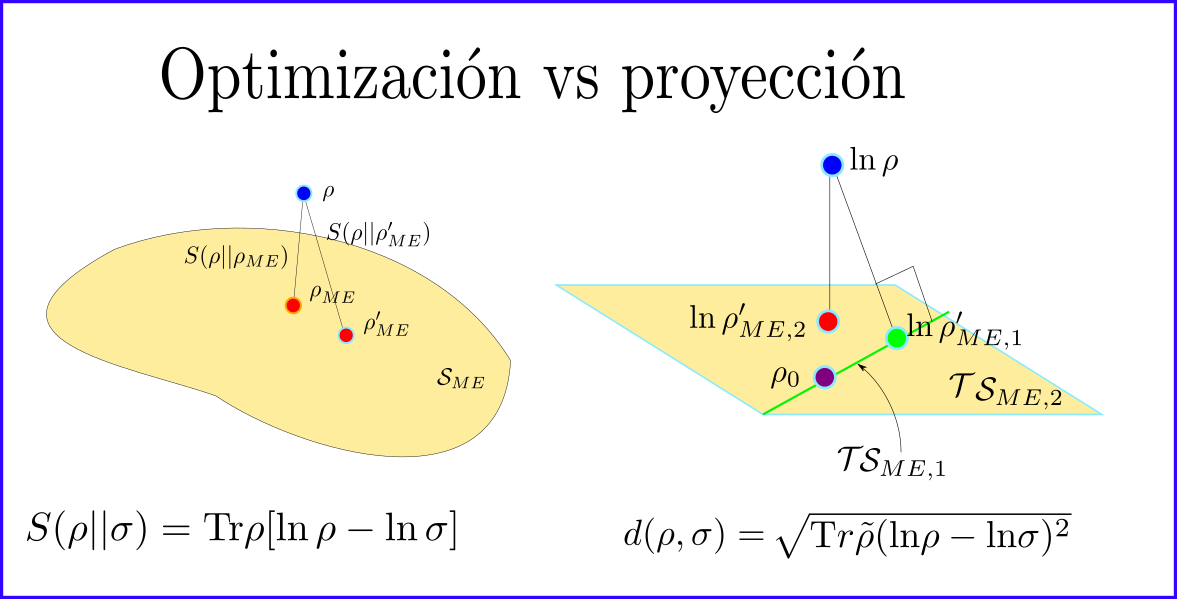
\includegraphics[scale=0.35]{figs/aprox-ME3-last.png}
    \caption{En esta figura mostramos dos situaciones. En la izquierda mostramos el procedimiento por optimización sobre el cual, Max-Ent halla su base. En la derecha planteamos una nueva situación. Disponemos de las variedades $\mathcal{S}_{ME,1}$ y $\mathcal{S}_{ME,2}$ ya definidas y de sus espacios tangentes asociados, denotados por $\mathcal{TS}_{ME,1}$ y $\mathcal{TS}_{ME,2}$. Sobre estos últimos podremos definir cantidades físicamente relevantes, entre ellas una noción de distancia entre estados a minimizar. Este último se logrará mediante un \textbf{Procedimiento de Proyección de uno y dos cuerpos}. }
    \label{aprox-ME3_page-0001}
\end{figure}

Dado que tanto los conjuntos Max-Ent de uno y dos cuerpos, $\mathcal{S}_{ME,1}$ y $\mathcal{S}_{ME,2}$, son variedades diferenciables Riemannianas podremos definir sus espacios tangentes asociados, denotados por $\mathcal{TS}_{ME,1}$ y $\mathcal{TS}_{ME,2}$ respectivamente, como se esquematiza en la figura \ref{aprox-ME3_page-0001}. Sobre estos podremos definir cantidades físicamente relevantes. En particular, sobre dichos espacios tangentes, podemos definir  productos internos de Hilbert Schmidt \eqref{HS scalar prod} y \eqref{HS scalar prod pond} y usar que todo producto interno induce una métrica o distancia bien definida. Nos interesará trabajar principalmente con \eqref{HS scalar prod pond} pues \eqref{HS scalar prod} es un caso especial, en el que el estado que pondera dicho producto  es $\rho = \mathds{1}$, y por tanto definimos la distancia entre estados

\begin{equation}
    d(\rho,\sigma) =   ||\log\rho-\log\sigma||_{\tilde{\rho}_{\textnormal{HS}}}
    , \label{state_distance}
\end{equation}

\noindent donde el estado estado de referencia $\tilde{\rho}$ se elige de según convenga, y puede cambiara o estar fijo fijo. Entonces, el Procedimiento de Proyección Ortogonal consiste en la optimización numérica de la función costo dada por \eqref{state_distance} en términos de ciertos parámetros, entre ellos las correlaciones de pares. La ventaja de este método es que las rutinas numéricas de proyección consumen muchos menos recursos informáticos que rutinas numéricas Max-Ent .

Las definiciones anteriores de distancia \eqref{state_distance} y producto escalar \eqref{HS scalar prod} son completamente válidas si son ponderadas por un estado cambiante con el tiempo, por lo que se implementó una rutina numérica recursiva basada en la continua actualización del estado que pondera estas cantidades precedentes por el estado inmediatamente anterior. Esto es: si se desea calcular la evolución del sistema a tiempo $t=t_i$ conociendo el estado del sistema al tiempo inmediatamente anterior $t_{i-1}$, luego la distancia y otras cantidades relacionadas estarán ponderadas por el estado inmediatamente anterior, $\rho(t_{i-1})$. Este procedimiento de actualizar el estado requiere de proyectar el estado y reconstruirlo mediante el producto tensorial. Este procedimiento de proyección y reconstrucción se podrá hacer sobre uno de los subsistemas o sobre ambos subsistemas \\

En síntesis, en esta sección usaremos distintos algoritmos y protocolos numéricos para ajustar los parámetros de un estado del estado de Gibbs \eqref{Gibbs_state} que mejor ajusten al verdadero estado del sistema, los cuales pasaremos a explicar a continuación.

\begin{tcolorbox}[title= Max-Ent de un cuerpo]
    En esta rutina numérica, que denotaremos como \textcolor{blue}{ME1}, disponemos de una base de $n$ operadores sobre el primer subsistema $\{\mathbf{O}_i^{(A)}\}_{i=1}^{n}\in \textnormal{HS}(\mathds{H}^{A})$ y de una base de $m$ operadores sobre el segundo subsistema $\{\mathbf{Q}_j^{(B)}\}_{j=1}^{m} \in \textnormal{HS}(\mathds{H}^{B})$. Luego, la base global será $n+m$-dimensional y estará dada los elementos
    
    $$
    \{\mathbf{O}_i^{(A)} \otimes \mathds{1}^{(B)}\}_{i=1}^{n} \cup \{\mathds{1}^{(A)} \otimes \mathbf{Q}_j^{(B)}\}_{j=1}^{m}
    $$
    
    y por tanto el estado de Gibbs tendrá $n+m$ parámetros $\{\lambda_{i}\}_{i=1}^{n+m} \in \mathds{R}$ a determinar. Se estudiará la dinámica restringida a la variedad $\mathcal{S}_{ME,1}$. La evolución del sistema cuántico será calculada mediante la función \texttt{mesolve} de la librería \texttt{QuTip} mientras que para la aproximación de la dinámica por estados gaussianos, se considera la entropía relativa \eqref{relative entropy} como función de costo a minimizar y los parámetros anteriores son calculados mediante la librería \texttt{scipy.optimize}. 
    
    \end{tcolorbox} \begin{tcolorbox}[title= Max-Ent de dos cuerpos] 
    En esta rutina numérica, que denotaremos como \textcolor{orange}{ME2}, disponemos de una base de $n$ operadores sobre el primer subsistema $\{\mathbf{O}_i^{(A)}\}_{i=1}^{n}\in \textnormal{HS}(\mathds{H}^{A})$ y de una base de $m$ operadores sobre el segundo subsistema $\{\mathbf{Q}_j^{(B)}\}_{j=1}^{m} \in \textnormal{HS}(\mathds{H}^{B})$ e incluímos términos de dos cuerpos. Luego, la base global será $n\times m+n+m$-dimensional y estará dada los elementos
    
    $$
    \{\mathbf{O}_i^{(A)} \otimes \mathds{1}^{(B)}\}_{i=1}^{n} \cup \{\mathds{1}^{(A)} \otimes \mathbf{Q}_j^{(B)}\}_{j=1}^{m} \cup \{\mathbf{O}_i^{(A)} \otimes \mathbf{Q}_j^{(B)}\}_{i=1, j=1}^{n,m}
    $$
    
    y por tanto el estado de Gibbs tendrá un total de $n \times m + n + m$ parámetros a ajustar, siendo estos $\{\lambda_{i}\}_{i=1}^{n+m} \in \mathds{R}$ y $\{\gamma_{ij}\}_{i=1,j=1}^{n,m} \in \mathds{R}$. Se estudiará la dinámica restringida a la variedad $\mathcal{S}_{ME,2}$. La evolución del sistema cuántico será calculada mediante la función \texttt{mesolve} de la librería \texttt{QuTip} mientras que para la aproximación de la dinámica por estados gaussianos, se considera la entropía relativa \eqref{relative entropy} como función de costo a minimizar y los parámetros anteriores son calculados mediante la librería \texttt{scipy.optimize}.
    \end{tcolorbox}
    \begin{tcolorbox}[title= Proyección Ortogonal de un cuerpo]
     En esta rutina numérica, que denotaremos como \textcolor{red}{TP1}, disponemos de una base de $n$ operadores sobre el primer subsistema $\{\mathbf{O}_i^{(A)}\}_{i=1}^{n}\in\textnormal{HS}(\mathds{H}^{A})$ y de una base de $m$ operadores sobre el segundo subsistema $\{\mathbf{Q}_j^{(B)}\}_{j=1}^{m} \in \textnormal{HS}(\mathds{H}^{B})$. Luego, la base global será $n+m$-dimensional y estará dada los elementos
    
    $$
    \{\mathbf{O}_i^{(A)} \otimes \mathds{1}^{(B)}\}_{i=1}^{n} \cup \{\mathds{1}^{(A)} \otimes \mathbf{Q}_j^{(B)}\}_{j=1}^{m}
    $$
    
    y por tanto el estado de Gibbs tendrá $n+m$ parámetros $\{\lambda_{i}\}_{i=1}^{n+m} \in \mathds{R}$ a determinar. Se estudiará la dinámica restringida a la variedad $\mathcal{S}_{ME,1}$. La evolución del sistema cuántico será calculada mediante la función \texttt{mesolve} de la librería \texttt{QuTip} mientras que para la aproximación de la dinámica por estados gaussianos, se considera a la distancia entre estados cuánticos, escrita en \eqref{state_distance} como función de costo a minimizar y los parámetros anteriores son calculados mediante la librería \texttt{scipy.optimize}.
     \end{tcolorbox}
    \begin{tcolorbox}[title= Proyección Ortogonal de dos cuerpos]
    En esta rutina numérica, que denotaremos como \textcolor{dark green}{TP2}, disponemos de una base de $n$ operadores sobre el primer subsistema $\{\mathbf{O}_i^{(A)}\}_{i=1}^{n}\in \textnormal{HS}(\mathds{H}^{A})$ y de una base de $m$ operadores sobre el segundo subsistema $\{\mathbf{Q}_j^{(B)}\}_{j=1}^{m} \in \textnormal{HS}(\mathds{H}^{B})$ e incluímos términos de dos cuerpos. Luego, la base global será $n\times m+n+m$-dimensional y estará dada los elementos
    
    $$
    \{\mathbf{O}_i^{(A)} \otimes \mathds{1}^{(B)}\}_{i=1}^{n} \cup \{\mathds{1}^{(A)} \otimes \mathbf{Q}_j^{(B)}\}_{j=1}^{m} \cup \{\mathbf{O}_i^{(A)} \otimes \mathbf{Q}_j^{(B)}\}_{i=1, j=1}^{n,m}
    $$
    
    y por tanto el estado de Gibbs tendrá un total de $n \times m + n + m$ parámetros a ajustar, siendo estos $\{\lambda_{i}\}_{i=1}^{n+m} \in \mathds{R}$ y $\{\gamma_{ij}\}_{i=1,j=1}^{n,m} \in \mathds{R}$. Se estudiará la dinámica restringida a la variedad $\mathcal{S}_{ME,2}$. La evolución del sistema cuántico será calculada mediante la función \texttt{mesolve} de la librería \texttt{QuTip} mientras que para la aproximación de la dinámica por estados gaussianos, se considera a la distancia entre estados cuánticos, escrita en \eqref{state_distance} como función de costo a minimizar y los parámetros anteriores son calculados mediante la librería \texttt{scipy.optimize}.
     \end{tcolorbox}

En la próxima sección estudiaremos cuan precisas y eficientes resultan ser estas estrategias para simular la dinámica real de distintos sistemas 
Para esto, analizaremos el comportamiento de las entropías relativas con el tiempo para cada rutina numérica, lo cual nos proveerá información de que tan similares son el estado obtenido por la rutina numérica y el estado exacto del sistema; como también las evoluciones temporales de los valores de expectación de ciertos operadores.

%{\color{red} \Large [Lo que sigue del capítulo debería tener esta estructura: \begin{itemize} \item 5.1) Sistema bosón-bosón truncados. No gaussianidad debida al truncado. 5.1.1) cerrado. no resonante 5.1.2 cerrado, resonante. 5.1.3) abierto resonante?.  \item 5.2) bosón-espín (Modelo de Dicke simplificado.) 5.1.1) "gaussiano" (acoplamiento conmuta con el Hamiltoniano de espín)   5.1. "no gaussiano" (acoplamiento no conmuta con el Hamiltoniano de espín) \end{itemize} En todos los casos, hay que establecer lo que valen los parámetros del estado inicial y de la evolución. }

\chapter{Aplicaciones}
\label{chapter5}


\begin{figure}
    \centering
    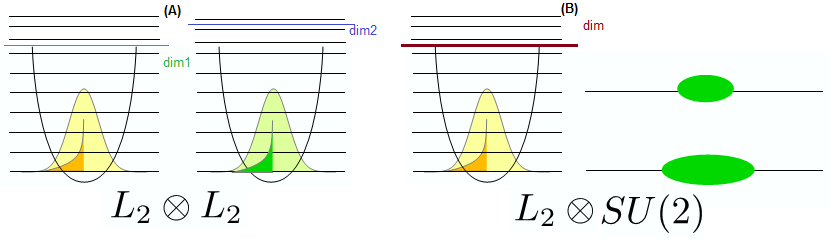
\includegraphics[scale=0.50]{figs/fig_models-cap5.png}
    \caption{En los presentes diagramas se muestran esquemas de la distribución de niveles de los sistemas estudiados en el presente capítulo. A la izquierda, se muestra el sistema de dos bosones, donde al estudiarlo numéricamente se realizará un truncamiento de los espacios de Hilbert bosónicos asociados a cada subsistema denotados por \texttt{dim1} y \texttt{dim2}. A la derecha, se muestra el sistema con acoplamiento bosón-espín, para el cual se implementará un truncamiento del espacio de Hilbert del subsistema bosónico denotado por el valor \texttt{dim}. Denotamos no rigurosamente las características de cada subsistema mediante $L_2$, el conocido espacio de Hilbert de la mecánica cuántica, para sistemas bosónicos y $SU(2)$, el grupo de simetría de los espines analizados.}
    \label{fig_models-cap5}
\end{figure}

En este capítulo aplicaremos los formalismos de aproximación de estados cuánticos anteriormente discutidos, en \autoref{ch_Max-Ent1} y \autoref{ch_Max-Ent2}, a situaciones concretas de sistemas físicos con dinámicas gaussianas o cuasi-gaussianas y dinámicas no gaussianas. En particular estudiaremos la dinámica de dos subsistemas bosónicos acoplados (figura \ref{fig_models-cap5}, izquierda) o un sistema bosón-espín (figura \ref{fig_models-cap5}, derecha), que admiten límites en los que una aproximación Max-Ent a la dinámica es exacta. Veremos luego cómo al truncar los sistemas bosónicos a dimensión finita esta propiedad de gaussianidad se pierde, lo que conlleva una pérdida de exactitud en la aproximación.
Analizaremos la eficacia de las aproximaciones implementadas para reproducir la dinámica de estos sistemas mediante los cálculos de entropía relativa y de la métrica de Bures-Wooters sobre dichos sistemas objetivos.

\section{Sistema de dos bosones}
\label{two_boson_system}

Como discutimos en el  \autoref{cap3_dosbosones}, la dinámica de un sistema bosónico átomo-cavidad que inicialmente se encuentra en un estado gaussiano, y cuya evolución está gobernada por un Hamiltoniano cuadrático en los operadores de creación y aniquilación bosónicos, constituye una dinámica Gaussiana; por lo que dicha dinámica siempre estará circunscrita a las variedades Max-Ent. La situación cambia radicalmente si el espectro de autoestados del sistema es finito-dimensional y discreto. En tal caso, los operadores de creación y aniquilación sobre cada modo bosónico son

\begin{subequations}
\begin{align}
{\bf a}_{i}\rightarrow {\bf a}^{N}_{i}=\sum_{n=0}^{N-1}\sqrt{n}|n\rangle_i \langle n+1|_i & \textnormal{ y }{\bf a}^{\dagger}_{i}\rightarrow {\bf a}^{\dagger N}_{i}=\sum_{n=0}^{N-1}\sqrt{n}|n+1\rangle_i \langle n|_i, \\
{\bf b}_{j}\rightarrow {\bf b}^{N}_{j}=\sum_{m=0}^{N-1}\sqrt{m}|m\rangle_j \langle m+1|_j & \textnormal{ y }{\bf b}^{\dagger}_{j}\rightarrow {\bf b}^{\dagger N}_{j}=\sum_{m=0}^{N-1}\sqrt{m}|m+1\rangle_j \langle m|_j,
\end{align}
\end{subequations}

donde se han de realizar las identificaciones ${\bf H}\rightarrow  {\bf H}={ \bf H}_1 + { \bf H}_2 + \lambda {\bf V}$, 
con ${\bf V}={\bf a}^{N\dagger}{\bf b}^{N}+{\bf b}^{N\dagger}{\bf a}^{N}$, 
${\bf H}_i=\sum_{k=0}^{N}\omega_i \bigg(n+\frac{1}{2}\bigg)|n \rangle_i\langle n|_i$, donde $\lambda$ es la constante de acoplamiento y siendo $\omega_i$ la frecuencia del $i$-ésimo modo de oscilación.

Sin embargo, en este caso aún podemos definir una variedad Riemanniana MaxEnt de estados asociados a los observables  $\{{\bf H}_1,{\bf H}_2,{\bf b}^{N\dagger}{\bf a}^{N},{\bf a}^{N\dagger}{\bf b}^{N}\}$, y forzar la dinámica sobre esta variedad mediante las dinámicas restringidas Max-Ent. 

Es importante destacar que este procedimiento de truncado de sistemas bosónicos a dimensión finita hará que las dinámicas estudiadas no sean gaussianas y consecuentemente se perderá exactitud en las aproximaciones usadas. 
Deseamos entonces estudiar qué tan aplicables son los protocolos implementados y cuantificar esta pérdida de exactitud asociada a la truncar la cantidad de niveles de energía asociado a cada sistema. A continuación estudiaremos varias dinámicas (cuasi-)gaussianas y no gaussianas para este sistema, a saber: 

\begin{itemize}
    \item En la \autoref{bxb_c_nr_g}, estudiaremos una dinámica cuasi-gaussiana cerrada no resonante.
    \item En la \autoref{bxb_cr}, estudiaremos una dinámica cuasi-gaussiana cerrada resonante.
    \item En la \autoref{bxb_or}, analizaremos una dinámica cuasi-gaussiana abierta no resonante
    \item y fianalmente en la  \autoref{bxb_cnr} estudiaremos una dinámica no gaussiana cerrada no resonante;
\end{itemize}

buscando analizar la efectividad de las rutinas numéricas implementadas en la descripción de estos sistemas. 

%\notamm{Esta sección de dinámica no gaussiana cerrada no resonante debería ir al final de esta subsección, justo antes del modelo de Dicke. El resto está OK.}

\clearpage

\subsection{Dinámica gaussiana cerrada no resonante}
\label{bxb_c_nr_g}

En esta sección estudiaremos la dinámica cerrada no resonante de un estado cuasi-gaussiano para el sistema de dos bosones. Para realizar los cálculos numéricos, hemos de truncar los espacios de Hilbert bosónicos a \texttt{dim1} y \texttt{dim2} niveles, donde \texttt{dim1} indica la cantidad de niveles de energía en el átomo y donde \texttt{dim2} indica la cantidad de niveles de energía en la cavidad. El estado inicial\footnote{A esta temperatura, $\beta=0.05$, la ocupación media bosónica es de 20 estados aproximadamente, mientras que en el estado truncado, el valor medio $\langle{\bf n_1} \rangle= 4$, lo cual es una condición lejana a la gaussianidad.} a considerar es 
\begin{equation}
\rho_{AB}(0) = e^{-0.05{\bf a}^{\texttt{dim1}\dagger} {\bf a}^{\texttt{dim1}}} \otimes e^{-0.05{\bf b}^{\texttt{dim2}\dagger} {\bf b}^{\texttt{dim2}}}
\label{model3.6_gaussian1}
\end{equation}

Nos interesa estudiar qué tan aplicables son los formalismos anteriores. Para las simulaciones, se tomaron los dimensiones de truncamiento \texttt{dim1}=\texttt{dim2}=10, frecuencias $\omega_1 = 3.0$ y $\omega_2 = \sqrt{48}$ y constante de acoplamiento $\lambda = 0.05$. En la figura \ref{rel_entropy_closed_nonres.png} se muestran los resultados de la entropía relativa global y parcial \textit{vs.} tiempo. 

\begin{figure}
    \centering
    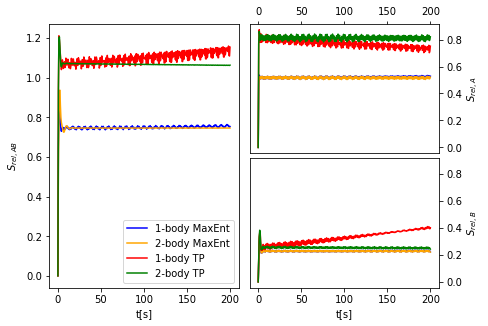
\includegraphics[scale=0.60]{figs/section3_4/section5_bxb-closed-nonres/rel_entropy_closed_nonres_g.png}
    \caption{En la presente figura mostramos la entropía relativa $S_{rel,AB}$, (izquierda) y las entropías parciales $S_{rel,A}$ (derecha superior) y $S_{rel,B}$ (derecha inferior) \textit{vs.} tiempo para la evolución cerrada no resonante del estado \eqref{model3.6_gaussian1} para el sistema de dos bosones. Se han usado las dimensiones de \textit{cut-off} \texttt{dim1} = \texttt{dim2} = 10, con frecuencias $\omega_1 = 3.0$ y $\omega_2 =\sqrt{48}$ y constante de acoplamiento $\lambda = 0.05$.}
    \label{rel_entropy_closed_nonres.png}
\end{figure}

De la figura \ref{rel_entropy_closed_nonres.png}, en particular para el \textit{plot} de la entropía global, notamos que los protocolos Max-Ent de uno y dos cuerpos, \textcolor{blue}{ME1} y \textcolor{orange}{ME2}, y Proyección ortogonal de dos  cuerpos, \textcolor{dark green}{TP2}, son útiles en la aproximación del estado del sistema, al no poseer una tendencia creciente a largos plazos en el tiempo. Para la entropía global tenemos que

\begin{gather*}
    \bigg|S(\rho_{\textnormal{\textcolor{blue}{ME1}}}|| \Tr_{1}\rho_{\textnormal{\textcolor{blue}{ME1}}} \otimes \Tr_{2}\rho_{\textnormal{\textcolor{blue}{ME1}}})(t) - S(\rho_{\textnormal{\textcolor{orange}{ME2}}}|| \Tr_{1}\rho_{\textnormal{\textcolor{orange}{ME2}}} \otimes \Tr_{2}\rho_{\textnormal{\textcolor{orange}{ME2}}})(t) \bigg| \leq 1 \times10^{-3} \textnormal{ y } \\  
    \bigg|S(\rho_{\textnormal{\textcolor{blue}{ME1}}}|| \Tr_{1}\rho_{\textnormal{\textcolor{blue}{ME1}}} \otimes \Tr_{2}\rho_{\textnormal{\textcolor{blue}{ME1}}})(t) 
    - S(\rho_{\textnormal{\textcolor{dark green}{TP2}}}|| \Tr_{1}\rho_{\textnormal{\textcolor{dark green}{TP2}}} \otimes \Tr_{2}\rho_{\textnormal{\textcolor{dark green}{TP2}}} (t) \bigg| \leq 0.4.
\end{gather*}

mientras que obtenemos resultados análogos para la entropía relativa parcial, calculada comparando los estados que describen a cada subsistema. Por otro lado, la rutina numérica de Proyección ortogonal de un cuerpo \textcolor{red}{TP1} resulta ser inadecuada al poseer una tendencia creciente y resulta divergente a largos plazos en el tiempo. Esto significa que los estados calculados mediante esta rutinas se vuelven progresivamente más distinguibles del estado exacto del sistema. \newline 

A raíz de estos resultados, nos interesa ahora estudiar el comportamiento de la evolución de la métrica de Bures-Wooters dada por \eqref{Bures-Wooters} acorde a tres métodos, que hayan su fundamento en los formalismos anteriores:

\begin{itemize}
    \item Primero, calcularemos la evolución de esta métrica con el tiempo usando la dinámica Max-Ent restringida de dos cuerpos. 
    %En particular calcularemos ${\bf B}(\rho_{\textnormal{\textcolor{orange}{ME2}}},  \exp{\log\rho_{\textnormal{\textcolor{orange}{ME2}}}-\lambda_i {\bf O_i}}) \textit{vs}. t$. 
    En los \textit{plots} futuros, denotamos a esta técnica como \textcolor{orange}{Max-Ent}.
    \item Luego, calcularemos la métrica de Bures-Wooters \textit{vs.} tiempo usando el procedimiento de Proyección Ortogonal de dos cuerpos, donde tanto la distancia definida en \eqref{state_distance} como el producto escalar de Hilbert-Schmidt dado por \eqref{HS scalar prod pond} están ponderados por un estado fijo $\rho_0$, el estado inicial. Es decir que calcularemos ${\bf B}(\rho_{\textnormal{exacto}}, \rho_{\textnormal{\textcolor{violet}{Proj rho0}}}) \textit{vs}. t$.  Será denotada como \textcolor{violet}{Proj rho0}.
    \item Finalmente, calcularemos la métrica de Bures-Wooters \textit{vs.} tiempo usando el procedimiento de proyección de dos cuerpos, donde ahora se actualizará el estado que pondera la distancia y el producto escalar de Hilbert-Schmidt dado por \eqref{HS scalar prod pond}. Esto es, para calcular el estado $\rho(t_i)$ a tiempo $t_i$, estas cantidades anteriores estarán ponderadas por el estado $\rho(t_{i-1})$. Es decir que calcularemos ${\bf B}(\rho_{\textnormal{exacto}}, \rho_{\textnormal{\textcolor{awesome}{Proj rho(t)}}}) \textit{vs}. t$.    Será denotada como \textcolor{awesome}{Proj rho(t)}.
\end{itemize}

Pasamos, a continuación, a estudiar el comportamiento de la métrica de Bures-Wooters \eqref{Bures-Wooters} \textit{vs.} tiempo acorde a los protocolos explicados en la sección anterior para conocer que tan cercanos son los estados calculados mediante dichas técnicas numéricas al estado exacto del sistema. 

\begin{figure}
\begin{minipage}{.5\linewidth}
\centering
\subfloat[]{\label{main:a}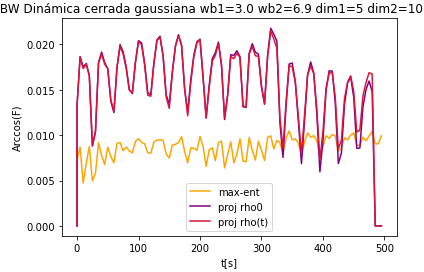
\includegraphics[align=t,scale=.68]{figs/section3_4/section5_bxb-closed-nonres/b5xb10_c_nonres_g.png}}
\end{minipage}%
\begin{minipage}{.5\linewidth}
\centering
\subfloat[]{\label{main:b}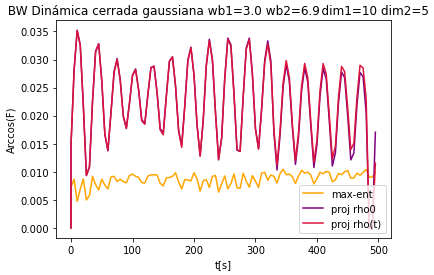
\includegraphics[align=t,scale=.68]{figs/section3_4/section5_bxb-closed-nonres/b10xb5_c_nonres_g.png}}
\end{minipage}\par\medskip
\centering
\subfloat[]{\label{main:c}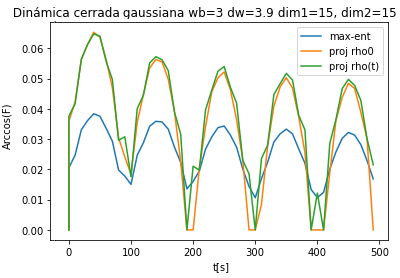
\includegraphics[align=t,scale=.68]{figs/section3_4/section5_bxb-closed-nonres/b15xb15_c_nonres_g.png}}
\caption{Se muestran los tres \textit{plots} de la métrica de Bures Wooters \textit{vs.} tiempo para distintos pares de truncamiento, (\texttt{dim1},\texttt{dim2}): (5,10) mostrado en (a), (10,5) mostrado en (b) y (15,15) mostrado en (c), en el caso de evolución cerrada no resonante del estado cuasi-gaussiano \eqref{model3.6_gaussian1} con frecuencias $\omega_1 = 3.0$,  $\omega_2 =\sqrt{48}$ y constante de acoplamiento $\lambda = 0.05$.}
\label{closed_n_nr}
\end{figure}

En la figura \ref{closed_n_nr} se muestran tres \textit{plots} de la métrica de Bures-Wooters \textit{vs.} tiempo acorde a los tres protocolos variando los parámetros de truncamiento. Para los tres pares de valores de truncamiento notamos que las dinámicas obtenidas a partir de Proyección Ortogonal de dos cuerpos, esto es \textcolor{violet}{Proj rho0} y \textcolor{awesome}{Proj rho(t)}, devuelven resultados muy similares entre sí, con una diferencia entre rutinas nunca superior a $2 \times 10^{-3}$. Por otro lado notamos que la diferencia entre los protocolos de Proyección Ortogonal y \textcolor{orange}{Max-Ent} nunca es superior a 0.10. Al aumentar los parámetros de truncamiento, las curvas de las métricas de Bures-Wooters empiezan a solaparse entre sí; lo cual es un resultado congruente con los obtenidos para la entropía relativa presentados en la figura \ref{rel_entropy_closed_nonres.png}.
\begin{figure}
    \centering
    \subfloat[\centering ]{{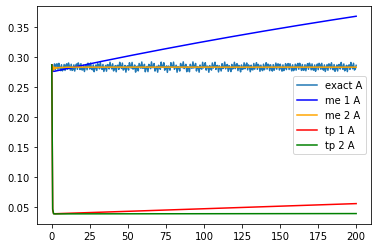
\includegraphics[scale=0.55]{figs/section3_4/section5_bxb-closed-nonres/n1_ocupation_number_closed_nonres_g.png} }}
    \qquad
    \subfloat[\centering ]{{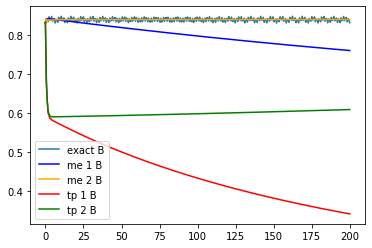
\includegraphics[scale=0.55]{figs/section3_4/section5_bxb-closed-nonres/n2_ocupation_number_closed_nonres_g.png}}}
    \caption{En esta figura se presentan los resultados para la evolución del valor de expectación $\lgg {\bf n}_1 \rgg$ (izquierda) y la evolución del valor de expectación $\lgg {\bf n}_2 \rgg$ (derecha), para truncamientos \texttt{dim1}=\texttt{dim2}=10, frecuencias $\omega_1 = 3.0\textnormal{ , } \omega_2 =\sqrt{48}$ y constante de acoplamiento $\lambda = 0.05$, con el tiempo para la evolución cerrada no resonante del estado cuasi gaussiano \eqref{model3.6_gaussian1} para el sistema de dos bosones.}
    \label{ocupations_closed_nonres}
\end{figure}

Por otro lado, en la figura \ref{ocupations_closed_nonres}, tenemos los resultados de la evolución temporal de los valores de expectación de los operadores ${\bf n}_1 = {\bf a}^{\texttt{dim1}\dagger} {\bf a}^{\texttt{dim1}}$ y ${\bf n}_2 = {\mathbf b}^{\texttt{dim2}\dagger} {\mathbf b}^{\texttt{dim2}}$, respectivamente, para parámetros de truncamiento \texttt{dim1}=\texttt{dim2}=10. 
Observamos que el protocolo Max-Ent de dos cuerpos \textcolor{orange}{ME2} es el que mejor ajusta las oscilaciones de la dinámica exacta, entorno a $0.27$ para $\langle{\bf n}_2\rangle$ y entorno a $0.85$ para $\langle{\bf n}_1\rangle$.
Notamos que Max-Ent de un cuerpo \textcolor{blue}{ME1} y \textcolor{red}{TP1} son inaplicables para modelar $\langle{\bf n}_1\rangle(t)$ y $\langle{\bf n}_2\rangle(t)$  respectivamente. Asimismo \textcolor{dark green}{TP2} es un formalismo aplicable pero que presenta deficiencias en reproducir los resultados exactos, sobretodo para modelar la evolución temporal del operador número $\langle{\bf n}_1\rangle(t)$. \\

\begin{table}
     \caption{Comportamiento asintótico de las entropías relativas Dinámica Gaussiana cerrada no resonante}
     \begin{tabular}{llllll}
        \toprule
         & \( \textcolor{blue}{\textbf{Max-Ent 1}} \) & \( \textcolor{red}{\textbf{Proy. Ortg. 1}} \) & \( \textcolor{orange}{\textbf{Max-Ent 2}} \) & \( \textcolor{dark green}{\textbf{Proy. Ortg. 2}} \)  \\
        \midrule   \\
        $S(\rho_{\cdots}||\sigma)\xrightarrow[t\gg 200 {s}]{} $  & $0.75 \pm 0.01$, & $\infty$, & $0.75 \pm 0.01$, & $1.10 \pm 0.01$.   \\
        $S(\rho_{\cdots_{A}}||\sigma_{A})\xrightarrow[t\gg 200 {s}]{} $ & $0.57 \pm 0.01$, & $0.60 \pm 0.05$, & $0.57 \pm 0.01$, & $0.81 \pm 0.01$. \\
        $S(\rho_{\cdots_{B}}||\sigma_{B})\xrightarrow[t\gg 200 {s}]{} $ & $0.21 \pm 0.01$, & $\infty$, & $0.21 \pm 0.01$, & $0.21 \pm 0.01$. \\
        \bottomrule
        & \( \textcolor{orange}{\textbf{Max-Ent}} \) & \( \textcolor{violet}{\textbf{Proy. Ortg. 2 }} \rho_0 \) & \( \textcolor{awesome}{\textbf{Proy. Ortg. 2 }} \rho(t) \) \\
        ${\bf B}(\rho_{\cdots}, \sigma)\textnormal{  } \xrightarrow[t\gg 200 {s}]{}$ & $0.09 \pm 0.01$, & $(1.1 \pm 0.1) \times 10^{-2}$, & $(1.1 \pm 0.1) \times 10^{-2}$, & {\small\textnormal{ para (\texttt{dim1}, \texttt{dim2}) = (5,10).}} \\
        & $(7 \pm 3)\times 10^{-3}$, & $(2.0 \pm 0.5)\times 10^{-2}$, & $(2.0 \pm 0.5)\times 10^{-2}$, & {\small\textnormal{ para (\texttt{dim1}, \texttt{dim2}) = (10,5).}}  \\
         & $(7 \pm 3)\times 10^{-3}$, & $(2.0 \pm 0.5)\times 10^{-2}$, & $(2.0 \pm 0.5)\times 10^{-2}$, & {\small\textnormal{ para (\texttt{dim1}, \texttt{dim2}) = (15,15).}} \\
        \bottomrule
        & \( \textcolor{blue}{\textbf{Max-Ent 1}} \) & \( \textcolor{red}{\textbf{Proy. Ortg. 1}} \) & \( \textcolor{orange}{\textbf{Max-Ent 2}} \) & \( \textcolor{dark green}{\textbf{Proy. Ortg. 2}} \) \\
        $\lgg {\bf n}_1 \rgg\xrightarrow[t\gg 200 {s}]{}$ & $\infty$, & $ 0.07 \pm 0.01 $, & $0.29 \pm 0.01$, & $ 0.03 \pm 0.01$.\\
        $\lgg {\bf n}_2 \rgg\xrightarrow[t\gg 200 {s}]{}$ & $ 0.65 \pm 0.01 $, & $ 0.30 \pm 0.10 $, & $0.85 \pm 0.01$, & $ 0.60 \pm 0.01$. \\
        \bottomrule
     \end{tabular} 
    \begin{tablenotes}
      \small
      \item En esta tabla presentamos los comportamientos asintóticos de las entropías relativas, de las métricas de Bures y los valores medios de los observables a tiempos largos ($t \gg 200s$) para las rutinas implementadas. Los primeros tres resultados corresponden a aquellos de la figura \ref{rel_entropy_closed_nonres.png}, los siguientes tres corresponden a la figura \ref{closed_n_nr} seguidos por aquellos mostrados en la figura \ref{ocupations_closed_nonres}. Los errores fueron calculados en base a las amplitudes de las oscilaciones. Los colores de las columnas están asociados a los colores de las curvas en las figuras. 
    \end{tablenotes}
    \label{table1}
\end{table}

Resumimos los resultados precedentes en la tabla \ref{table1}. Concluimos entonces que para la dinámica dada por la evolución del estado \eqref{model3.6_gaussian1}, una dinámica de por sí lejana a la gaussianidad, se obtuvo que los formalismos de dos cuerpos son capaces de describir correctamente la evolución del sistema.

\subsection{Dinámica cerrada gaussiana resonante}
\label{bxb_cr}

Estudiaremos ahora la evolución de la dinámica cuasi gaussiana cerrada resonante con dimensiones de \textit{cut-off} iniciales de \texttt{dim1}=\texttt{dim2}=10, frecuencias $\omega_1 = \omega_2 = 3.0$ y acoplamiento $\lambda = 0.05$. Se toma al estado inicial descorrelacionado dado por \eqref{model3.6_gaussian1}. Nuevamente, dicha dinámica es cuasi-gaussiana y se busca estudiar que tan aplicables son las rutinas numéricas en la descripción de esta. Se presentan los resultados obtenidos. 

\begin{figure}
    \centering
    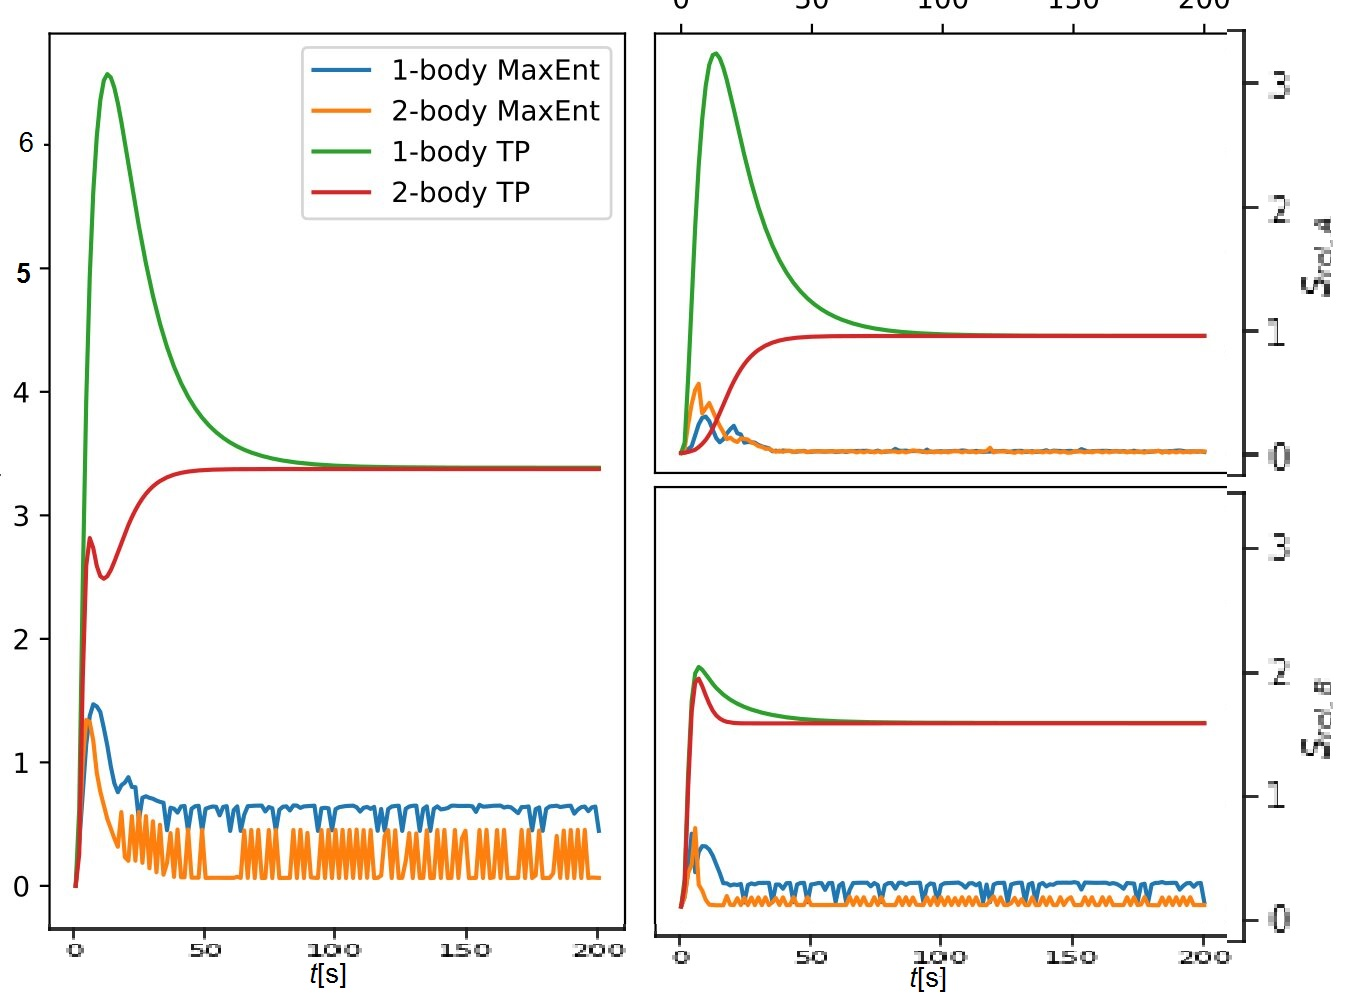
\includegraphics[scale=0.65]{figs/section3_4/section5_bxb-closed-res/rel_entropy_closed_res_g.jpg}
    \caption{En la presente figura mostramos la entropía relativa $S_{rel,AB}$, (izquierda) y las entropías parciales $S_{rel,A}$ (derecha superior) y $S_{rel,B}$ (derecha inferior) \textit{vs.} tiempo para la evolución cerrada resonante del estado \eqref{model3.6_gaussian1} para el sistema de dos bosones. Se han usado las dimensiones de \textit{cut-off} \texttt{dim1} = \texttt{dim2} = 10, con frecuencias $\omega_1 = \omega_2 = 3.0$ y constante de acoplamiento $\lambda = 0.05$.}
    \label{rel_entropy_closed_res}
\end{figure}

De la figura \ref{rel_entropy_closed_res} observamos que las rutinas de Max-Ent \textcolor{blue}{ME1} y \textcolor{orange}{ME2} se estabilizan entorno a $0.9$ para la entropía relativa global y entorno a $0.5$ para las entropías relativas parciales para tiempos superiores a 100s; siendo la curva obtenida para \textcolor{blue}{ME1} ligeramente superior a la obtenida para \textcolor{orange}{ME2}, lo cual es un resultado esperable. Por otro lado, los protocolos de Proyección Ortogonal de uno y dos cuerpos  \textcolor{red}{TP1} y \textcolor{dark green}{TP2} devuelven virtualmente dinámicas idénticas entre sí, estabilizándose ambas entorno a $1.5$ para la entropía relativa global y en torno a $1.0$ para las entropías relativas parciales para tiempos mayores a 100s. 
Por tanto, los estados obtenidos mediante estas rutinas son poco distinguibles del estado exacto del sistema. En particular para las entropías relativas globales tenemos que 

%\bigg|S(\rho_{\textnormal{\textcolor{blue}{ME1}}}|| \Tr_{1}\rho_{\textnormal{\textcolor{blue}{ME1}}} \otimes \Tr_{2}\rho_{\textnormal{\textcolor{blue}{ME1}}})(t) - S(\rho_{\textnormal{\textcolor{orange}{ME2}}}|| \Tr_{1}\rho_{\textnormal{\textcolor{orange}{ME2}}} \otimes \Tr_{2}\rho_{\textnormal{\textcolor{orange}{ME2}}})(t) \bigg| \leq 1 \times10^{-3} \textnormal{ y }

\begin{gather*}
     \bigg|S(\rho_{\textnormal{\textcolor{blue}{ME1}}}|| \Tr_{1}\rho_{\textnormal{\textcolor{blue}{ME1}}} \otimes \Tr_{2}\rho_{\textnormal{\textcolor{blue}{ME1}}})(t) - S(\rho_{\textnormal{\textcolor{orange}{ME2}}}|| \Tr_{1}\rho_{\textnormal{\textcolor{orange}{ME2}}} \otimes \Tr_{2}\rho_{\textnormal{\textcolor{orange}{ME2}}})(t)  \bigg|  \leq 0.1 \\
     \bigg|  S(\rho_{\textnormal{\textcolor{red}{TP1}}}|| \Tr_{1}\rho_{\textnormal{\textcolor{red}{TP1}}} \otimes \Tr_{2}\rho_{\textnormal{\textcolor{red}{TP1}}})(t) -
     S(\rho_{\textnormal{\textcolor{dark green}{TP2}}}|| \Tr_{1}\rho_{\textnormal{\textcolor{dark green}{TP2}}} \otimes \Tr_{2}\rho_{\textnormal{\textcolor{dark green}{TP2}}})(t) \bigg|  \leq 1 \times10^{-3} \textnormal{ y} \\ \bigg|S(\rho_{\textnormal{\textcolor{blue}{ME1}}}|| \Tr_{1}\rho_{\textnormal{\textcolor{blue}{ME1}}} \otimes \Tr_{2}\rho_{\textnormal{\textcolor{blue}{ME1}}})(t) -
     S(\rho_{\textnormal{\textcolor{dark green}{TP2}}}|| \Tr_{1}\rho_{\textnormal{\textcolor{dark green}{TP2}}} \otimes \Tr_{2}\rho_{\textnormal{\textcolor{dark green}{TP2}}})(t) \bigg| \leq 1.0.
\end{gather*}

\begin{figure}
\begin{minipage}{.5\linewidth}
\centering
\subfloat[]{\label{main:a}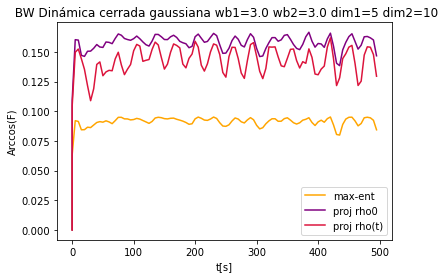
\includegraphics[scale=.52]{figs/section3_4/section5_bxb-closed-res/b5xb10_c_res_g.png}}
\end{minipage}%
\begin{minipage}{.5\linewidth}
\centering
\subfloat[]{\label{main:b}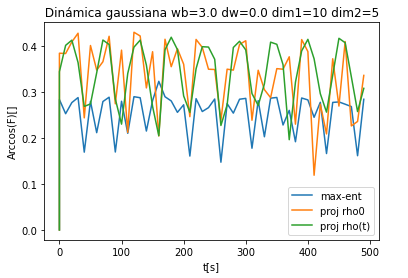
\includegraphics[scale=.52]{figs/section3_4/section5_bxb-closed-res/b10xb5_c_res_g.png}}
\end{minipage}\par\medskip
\centering
\subfloat[]{\label{main:c}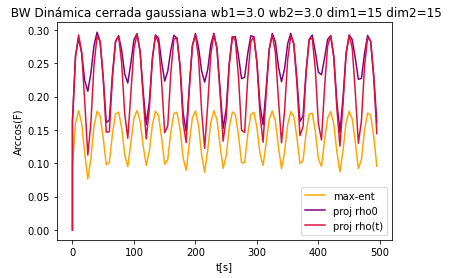
\includegraphics[scale=.52]{figs/section3_4/section5_bxb-closed-res/b15xb15_c_res_g.png}}
\caption{Se muestran los tres \textit{plots} de la métrica de Bures Wooters \textit{vs.} tiempo para distintos pares de truncamiento, (\texttt{dim1},\texttt{dim2}): (5,10) mostrado en (a), (10,5) mostrado en (b) y (15,15) mostrado en (c), en el caso de evolución cerrada resonante del estado cuasi-gaussiano \eqref{model3.6_gaussian1} con frecuencias $\omega_1 = \omega_2 = 3.0$ y  acoplamiento $\lambda = 0.05$.}
\label{bxb-closed-res/bxb_closed_r.png}
\end{figure}

A raíz de estos resultados favorables obtenidos de la entropía relativa, nuevamente estudiamos el comportamiento de la métrica de Bures-Wooters y su evolución con el tiempo acorde a los protocolos de dinámica Max-Ent restringida de dos cuerpos \textcolor{orange}{ME2} y por Proyección Ortogonal, los protocolos \textcolor{violet}{Proj rho0} y \textcolor{awesome}{Proj rho(t)}. En la figura \ref{bxb-closed-res/bxb_closed_r.png} se muestran dichos resultados. Como se puede apreciar, la diferencia entre protocolos es mínima - nunca mayor a $0.2$ -. Adicionalmente, al aumentar los parámetros de truncado notamos que estas diferencias entre protocolos disminuyen aún más - notar el solapamiento de las curvas obtenidas para el tercer \textit{plot}, el caso de (\texttt{dim1},\texttt{dim2})=(15,15) - como era de esperar siendo estos resultados congruentes con aquellos obtenidos de la entropía relativa.

\begin{figure}
    \centering
    \subfloat[\centering ]{{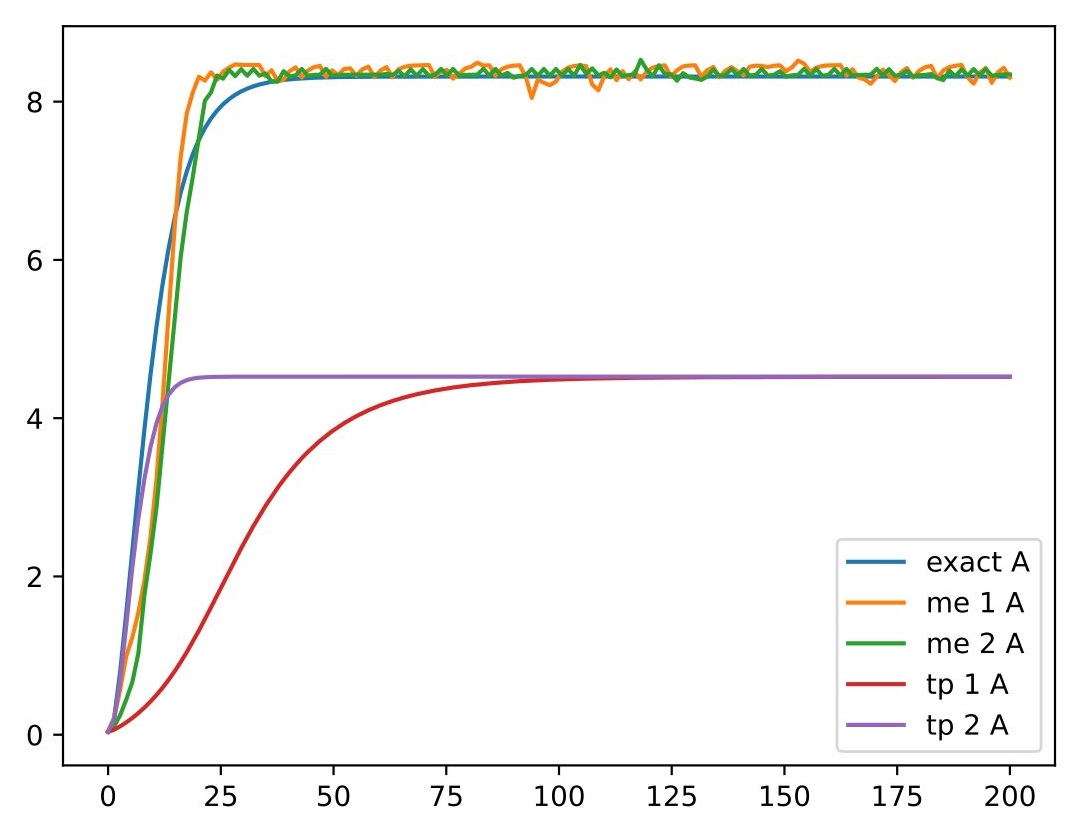
\includegraphics[scale=0.55]{figs/section3_4/section5_bxb-closed-res/n1_ocupation_number_closed_res_g.jpg}}}
    \qquad
    \subfloat[\centering ]{{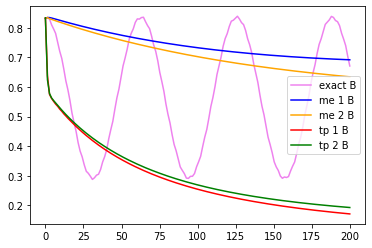
\includegraphics[scale=0.55]{figs/section3_4/section5_bxb-closed-res/n2_ocupation_number_closed_res_g.jpg}}}
    \caption{En esta figura se presentan los resultados para la evolución del valor de expectación $\lgg {\bf n}_1 \rgg$ (figura de la izquierda) y la evolución del valor de expectación $\lgg {\bf n}_2 \rgg$ (figura de la derecha) con el tiempo para la evolución cerrada resonante de un estado no gaussiano para el sistema de dos bosones. Se han usado las dimensiones de \textit{cut-off} \texttt{dim1}= \texttt{dim2} = 10, frecuencias $\omega_1 = \omega_2 = 3.0$ y acoplamiento $\lambda = 0.05$.}
    \label{ocupations_closed_res}
\end{figure}

En la figura \ref{ocupations_closed_res} tenemos los resultados de la evolución temporal de los valores de expectación de los operadores ${\bf n}_1 = {\bf a}^{\texttt{dim1}\dagger} {\bf a}^{\texttt{dim1}}$ y ${\bf n}_2 = {\mathbf b}^{\texttt{dim2}\dagger} {\mathbf b}^{\texttt{dim2}}$ respectivamente. De dichos gráficos observamos que las rutinas de Max-Ent de uno y dos cuerpos, \textcolor{blue}{ME1} y \textcolor{orange}{ME2}, devuelven resultados acordes a la dinámica exacta del sistema, estabilizándose entorno a $0.6$, tanto para $\lgg{\bf n}_1\rgg$ como para $\lgg{\bf n}_2\rgg$. Por otro lado, las rutinas de Proyección Ortogonal \textcolor{red}{TP1} y \textcolor{dark green}{TP2} no reproducen los resultados correctos, estabilizándose por debajo del mínimo de las oscilaciones. 

\begin{table}
     \caption{Comportamiento asintótico de las entropías relativas Dinámica Gaussiana cerrada no resonante}
     \begin{tabular}{llllll}
        \toprule
         & \( \textcolor{blue}{\textbf{Max-Ent 1}} \) & \( \textcolor{red}{\textbf{Proy. Ortg. 1}} \) & \( \textcolor{orange}{\textbf{Max-Ent 2}} \) & \( \textcolor{dark green}{\textbf{Proy. Ortg. 2}} \)  \\
        \midrule   \\
        $S(\rho_{\cdots}||\sigma)\xrightarrow[t\gg 200 {s}]{} $ & $0.85 \pm 0.10$, & $1.5 \pm 0.1$, & $0.85 \pm 0.10$, & $1.5 \pm 0.1$.   \\
        $S(\rho_{\cdots_{A}}||\sigma_{A})\xrightarrow[t\gg 200 {s}]{} $ & $0.4 \pm 0.05$, & $0.8 \pm 0.02$, & $0.4 \pm 0.05$, & $0.8 \pm 0.02$. \\
        $S(\rho_{\cdots_{B}}||\sigma_{B})\xrightarrow[t\gg 200 {s}]{} $ & $0.30 \pm 0.05$, & N/A, & $0.30 \pm 0.05$, & N/A. \\
        \bottomrule
        & \( \textcolor{orange}{\textbf{Max-Ent}} \) & \( \textcolor{violet}{\textbf{Proy. Ortg. 2 }} \rho_0 \) & \( \textcolor{awesome}{\textbf{Proy. Ortg. 2 }} \rho(t) \) \\
        ${\bf B}(\rho_{\cdots}, \sigma)\textnormal{  } \xrightarrow[t\gg 200 {s}]{}$ & $0.08 \pm 0.01$, & $0.13 \pm 0.05$, & $0.16 \pm 0.03$, & {\small\textnormal{ para (\texttt{dim1}, \texttt{dim2}) = (5,10).}} \\
        & $0.08 \pm 0.01$, & $0.12 \pm 0.04$, & $0.13 \pm 0.02$, & {\small\textnormal{ para (\texttt{dim1}, \texttt{dim2}) = (10,5).}}  \\
        & $0.13 \pm 0.02$, & $0.25 \pm 0.10$, & $0.20 \pm 0.05$, & {\small\textnormal{ para (\texttt{dim1}, \texttt{dim2}) = (15,15).}} \\
        \bottomrule
        & \( \textcolor{blue}{\textbf{Max-Ent 1}} \) & \( \textcolor{red}{\textbf{Proy. Ortg. 1}} \) & \( \textcolor{orange}{\textbf{Max-Ent 2}} \) & \( \textcolor{dark green}{\textbf{Proy. Ortg. 2}} \) \\
        $\lgg {\bf n}_1 \rgg\xrightarrow[t\gg 200 {s}]{}$ & $0.60 \pm 0.05$, & $0.10 \pm 0.01$, & $0.60 \pm 0.05$, & $0.10 \pm 0.01$.\\
        $\lgg {\bf n}_2 \rgg\xrightarrow[t\gg 200 {s}]{}$ & $0.60 \pm 0.05$, & $0.10 \pm 0.01$, & $0.60 \pm 0.05$, & $0.10 \pm 0.01$.\\ \\
        \bottomrule
     \end{tabular} 
    \begin{tablenotes}
      \small
      \item En esta tabla presentamos los comportamientos asintóticos de las entropías relativas, de las métricas de Bures y los valores medios de los observables a tiempos largos para las rutinas implementadas, donde $\rho$ es el estado calculado acorde a la rutina indexada en la columna y siendo $\sigma$ el estado exacto del sistema. Los resultados corresponden a aquellos de la figura \ref{rel_entropy_closed_res}, los siguientes tres corresponden a la figura \ref{bxb-closed-res/bxb_closed_r.png} seguidos por aquellos mostrados en la figura \ref{ocupations_closed_res}. Los errores fueron calculados teniendo el cuenta el máximo de las oscilaciones. Los colores de las columnas están asociados a los colores de las curvas respectivas. 
    \end{tablenotes}
    \label{table2}
\end{table}

En la tabla \ref{table2}, mostramos estos resultados. Concluimos de estos análisis que las cuatro rutinas implementadas son capaces de simular esta dinámica en lo que refiere al cálculo del estado del sistema y cálculo de evoluciones de operadores, a un costo computacional mucho menor que Max-Ent. 

\subsection{Dinámica abierta gaussiana no resonante }
\label{bxb_or}

En esta sección estudiaremos la dinámica abierta no resonante para el sistema de dos bosones con operadores de colapso bosónicos del primer subsistema - esto es ${\bf C}_1 = {\bf a}^{\texttt{dim1}}$, ${\bf C}_2 = {\bf a}^{\texttt{dim1}\dagger}$ -  y donde se han tomado las dimensiones de truncamiento iniciales \texttt{dim1}=\texttt{dim2}=10, frecuencias $\omega_1 = 3.0$, $\omega_2 = \sqrt{48}$ y factores de colapso $\gamma_1 = 0.1$, $\gamma_2 = 2 \gamma_1$ con un acoplamiento $\lambda = 0.05$. Se toma la dinámica cuasi-gaussiana de un estado inicial \eqref{model3.6_gaussian1}. Pasamos a discutir los resultados.

\begin{figure}
    \centering
    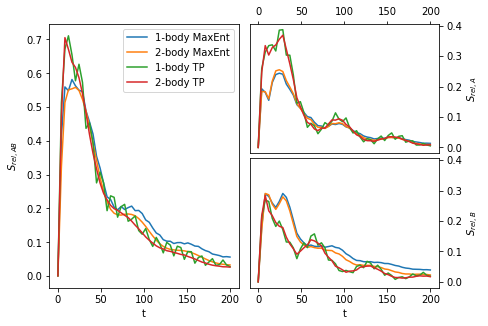
\includegraphics[scale=0.6]{figs/section3_4/section5_bxb-open-nonres/rel_entropy_open_nonres_ng.png}
    \caption{En la presente figura mostramos la entropía relativa $S_{rel,AB}$, (izquierda) y las entropías parciales $S_{rel,A}$ (derecha superior) y $S_{rel,B}$ (derecha inferior) \textit{vs.} tiempo para la evolución abierta no resonante del estado \eqref{model3.6_gaussian1} para el sistema de dos bosones, usando operadores de colapso bosónicos del primer subsistema. Se han usado las dimensiones de \textit{cut-off} \texttt{dim1}=\texttt{dim2}=10, frecuencias $\omega_1 = 3.0$, $\omega_2 = \sqrt{48}$ y factores de colapso $\gamma_1 = 0.1$, $\gamma_2 = 2 \gamma_1$ con un acoplamiento $\lambda = 0.05$.}
    \label{rel_entropy_open_nonres}
\end{figure}

De la figura \ref{rel_entropy_open_nonres} notamos que los protocolos \textcolor{blue}{ME1}, \textcolor{orange}{ME2} y \textcolor{dark green}{TP2}  devuelven virtualmente las mismas dinámicas para tiempos superiores a 150s, tendiendo a estabilizarse entorno a $0.4$ a largos plazos para la entropía relativa global. Resultados análogos fueron obtenidos para las entropías relativas parciales, donde estos tres protocolos tienden a estabilizarse entorno a $0.2$.
Por otro el protocolo \textcolor{red}{TP1} también no resulta ser un formalismo aplicable, al estabilizarse entorno a $0.6$ para la entropía global pero diverge para la entropía parcial al segundo subsistema. Esto es, para las entropías globales y parciales tenemos que 

\begin{gather*}
    \bigg|S(\rho_{\textnormal{\textcolor{blue}{ME1}}}|| \Tr_{1}\rho_{\textnormal{\textcolor{blue}{ME1}}} \otimes \Tr_{2}\rho_{\textnormal{\textcolor{blue}{ME1}}})(t) - S(\rho_{\textnormal{\textcolor{orange}{ME2}}}|| \Tr_{1}\rho_{\textnormal{\textcolor{orange}{ME2}}} \otimes \Tr_{2}\rho_{\textnormal{\textcolor{orange}{ME2}}})(t) \bigg| \leq 1 \times10^{-3} \textnormal{ y } \\  
    \bigg|S(\rho_{\textnormal{\textcolor{blue}{ME1}}}|| \Tr_{1}\rho_{\textnormal{\textcolor{blue}{ME1}}} \otimes \Tr_{2}\rho_{\textnormal{\textcolor{blue}{ME1}}})(t) 
    - S(\rho_{\textnormal{\textcolor{dark green}{TP2}}}|| \Tr_{1}\rho_{\textnormal{\textcolor{dark green}{TP2}}} \otimes \Tr_{2}\rho_{\textnormal{\textcolor{dark green}{TP2}}} (t) \bigg| \leq 1 \times10^{-3}.
\end{gather*}

Luego, los primeros tres protocolos devuelven dinámicas fidedignas a la exacta y además, notamos que la evolución a largos plazos de esta dinámica está regida únicamente por correlaciones de pares, siendo los efectos de los términos de mayor orden insignificantes. A partir de estos resultados prometedores, pasamos a estudiar el comportamiento de la métrica de Bures-Wooters con el tiempo usando los protocolos explicados en la \autoref{bxb_cnr}. 

\begin{figure}
\begin{minipage}{.5\linewidth}
\centering
\subfloat[]{\label{main:a}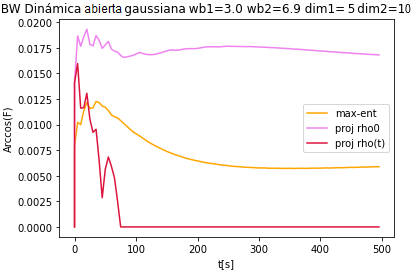
\includegraphics[scale=.7]{figs/section3_4/section5_bxb-open-nonres/b5xb10_open_nonres_g.png}}
\end{minipage}%
\begin{minipage}{.5\linewidth}
\centering
\subfloat[]{\label{main:b}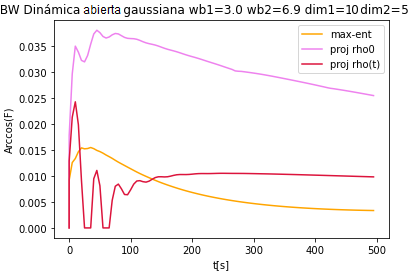
\includegraphics[scale=.7]{figs/section3_4/section5_bxb-open-nonres/b10xb5_open_nonres_g.png}}
\end{minipage}\par\medskip
\centering
\subfloat[]{\label{main:c}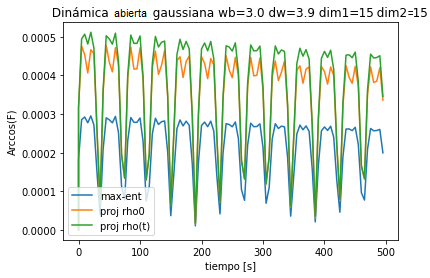
\includegraphics[scale=.7]{figs/section3_4/section5_bxb-open-nonres/b15xb15_open_nonres_g.png}}
\caption{Se muestran tres \textit{plots} de la métrica de Bures-Wooters \textit{vs.} tiempo para distintos pares de parámetros de truncamiento (\texttt{dim1},\texttt{dim2}): (5,10) mostrado en (a), (10,5) mostrado en (b) y (15,15) mostrado en (c), para la evolución abierta no resonante del estado cuasi gaussiano dado por \eqref{model3.6_gaussian1} con frecuencias $\omega_1 = 3.0$, $\omega_2 = \sqrt{48}$ y factores de colapso $\gamma_1 = 0.1$, $\gamma_2 = 2 \gamma_1$ con un acoplamiento $\lambda = 0.05$. }
\label{bxb-closed-res/bxb_open_nr.png}
\end{figure}

Como vemos de los tres gráficos presentados en la figura \ref{bxb-closed-res/bxb_open_nr.png},
las dos dinámicas de Proyección Ortogonal \textcolor{violet}{Proj rho0} y \textcolor{awesome}{Proj rho(t)} devuelven resultados muy similares entre sí, con una diferencia nunca mayor a $1\times 10^{-2}$ para los casos de truncamiento $(\texttt{dim1},\texttt{dim2})=(5,10),(10,5)$. La diferencia con Max-Ent va disminuyendo progresivamente a medida que aumentan los parámetros de truncamiento. En el tercer caso, con truncamientos $(\texttt{dim1},\texttt{dim2})=(15,15)$ esta es del orden de $0.20$ pero notando que las dinámicas tienden a oscilar bruscamente. Estos resultados son excelentes, implicando esto la aplicabilidad de dichas rutinas en la aproximación de la dinámica exacta sin deterioro significativo en la calidad de resultados, resultados acordes a los obtenidos para la entropía relativa en la figura \ref{rel_entropy_open_nonres}.

\begin{figure}
    \centering
    \subfloat[\centering ]{{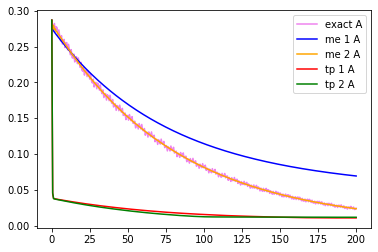
\includegraphics[scale=0.55]{figs/section3_4/section5_bxb-open-nonres/n1_ocupation_number_open_nonres_ng.png} }}
    \qquad
    \subfloat[\centering]{{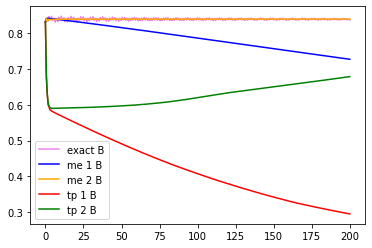
\includegraphics[scale=0.55]{figs/section3_4/section5_bxb-open-nonres/n2_ocupation_number_open_nonres_ng.png} }}
    \caption{En esta figura se presentan los resultados para la evolución del valor de expectación $\lgg {\bf n}_1 \rgg$ (figura izquierda) y la evolución del valor de expectación $\lgg {\bf n}_2 \rgg$ (figura derecha) con el tiempo para la evolución abierta resonante de un estado gaussiano usando operadores de colapso dados por operadores bosónicos del primer subsistem. Se usan las dimensiones de truncamiento \texttt{dim1}=\texttt{dim2}=10, frecuencias $\omega_1 = 3.0$, $\omega_2 = \sqrt{48}$ y factores de colapso $\gamma_1 = 0.1$, $\gamma_2 = 2 \gamma_1$ y constante de acoplamiento $\lambda = 0.05$.}
    \label{ocupations_open1_res}
\end{figure}

Por otro lado, de la figura \ref{ocupations_open1_res},  tenemos los resultados de la evolución temporal de los valores de expectación de los operadores ${\bf n}_1 = {\bf a}^{\texttt{dim1}\dagger} {\bf a}^{\texttt{dim1}}$ y ${\bf n}_2 = {\mathbf b}^{\texttt{dim2}\dagger} {\mathbf b}^{\texttt{dim2}}$, respectivamente. 
Notamos que las cuatro dinámicas devuelven resultados similares para el valor de expectación ${\bf n}_1 = {\bf a}^{\texttt{dim1}\dagger} {\bf a}^{\texttt{dim1}}$, no así para ${\bf n}_2 = {\mathbf b}^{\texttt{dim2}\dagger} {\mathbf b}^{\texttt{dim2}}$. En el primer caso, los protocolos Max-Ent \textcolor{blue}{ME1} y \textcolor{orange}{ME2} tienden a estabilizarse por encima de los resultados exactos mientras que Proyección Ortogonal \textcolor{red}{TP1} y \textcolor{dark green}{TP2} ajustan mejor a la dinámica exacta a tiempos largos $t\gg 200s$. Para el segundo caso, \textcolor{blue}{ME1} y \textcolor{red}{TP1} resultan inaplicables a largos plazos pero los protocolos de dos cuerpos \textcolor{orange}{ME2} y \textcolor{dark green}{TP2} devuelven buenos resultados.\\

\begin{table}
     \caption{Comportamiento asintótico de las entropías relativas Dinámica Gaussiana cerrada no resonante}
     \begin{tabular}{llllll}
        \toprule
         & \( \textcolor{blue}{\textbf{Max-Ent 1}} \) & \( \textcolor{red}{\textbf{Proy. Ortg. 1}} \) & \( \textcolor{orange}{\textbf{Max-Ent 2}} \) & \( \textcolor{dark green}{\textbf{Proy. Ortg. 2}} \)  \\
        \midrule   \\
        $S(\rho_{\cdots}||\sigma)\xrightarrow[t\gg 200 {s}]{} $  & $1.00 \pm 0.01$, & $0.60 \pm 0.05$, & $1.00 \pm 0.01$, & $1.00 \pm 0.01$.   \\
        $S(\rho_{\cdots_{A}}||\sigma_{A})\xrightarrow[t\gg 200 {s}]{} $ & $0.15 \pm 0.01$, & $0.15 \pm 0.01$ &, $0.15 \pm 0.01$, & $0.15 \pm 0.01$. \\
        $S(\rho_{\cdots_{B}}||\sigma_{B})\xrightarrow[t\gg 200 {s}]{} $ & $0.21 \pm 0.01$, & $\infty$, & $0.21 \pm 0.01$, & $0.21 \pm 0.01$.\\
        \bottomrule
        & \( \textcolor{orange}{\textbf{Max-Ent}} \) & \( \textcolor{violet}{\textbf{Proy. Ortg. 2 }} \rho_0 \) & \( \textcolor{awesome}{\textbf{Proy. Ortg. 2 }} \rho(t) \) \\
        ${\bf B}(\rho_{\cdots}, \sigma)\textnormal{  } \xrightarrow[t\gg 200 {s}]{}$ & $(8.0 \pm 0.1) \times 10^{-3}$, &$(1.75 \pm 0.01) \times 10^{-2}$, & 0, & {\small\textnormal{ para (\texttt{dim1}, \texttt{dim2}) = (5,10).}} \\
        & $(1.0 \pm 0.1) \times 10^{-2}$, & $(2.0 \pm 0.1) \times 10^{-2}$, & $(5.0 \pm 0.1) \times 10^{-3}$, & {\small\textnormal{ para (\texttt{dim1}, \texttt{dim2}) = (10,5).}}  \\
         &$0.20 \pm 0.20$ & $0$,& $0$, & {\small\textnormal{ para (\texttt{dim1}, \texttt{dim2}) = (15,15).}} \\
        \bottomrule
        & \( \textcolor{blue}{\textbf{Max-Ent 1}} \) & \( \textcolor{red}{\textbf{Proy. Ortg. 1}} \) & \( \textcolor{orange}{\textbf{Max-Ent 2}} \) & \( \textcolor{dark green}{\textbf{Proy. Ortg. 2}} \) \\
        $\lgg {\bf n}_1 \rgg\xrightarrow[t\gg 200 {s}]{}$ & $0.08 \pm 0.01$, & $0.03 \pm 0.01$ & $0.4 \pm 0.01$, & $0.03 \pm 0.01$.\\
        $\lgg {\bf n}_2 \rgg\xrightarrow[t\gg 200 {s}]{}$ & $0.6 \pm 0.1$, & $0.2\pm 0.1$ & $0.85 \pm 0.01$, & $0.7 \pm 0.1$.\\ \\
        \bottomrule
     \end{tabular} 
    \begin{tablenotes}
      \small
      \item En esta tabla presentamos los comportamientos asintóticos de las entropías relativas, de las métricas de Bures y los valores medios de los observables a tiempos largos para las rutinas implementadas. Los resultados corresponden a aquellos de la figura \ref{rel_entropy_open_nonres}, los siguientes tres corresponden a la figura \ref{bxb-closed-res/bxb_open_nr.png} seguidos por aquellos mostrados en la figura \ref{ocupations_open1_res}. Los errores fueron calculados teniendo el cuenta el máximo de las oscilaciones. Los colores de las columnas están asociados a los colores de las curvas respectivas. 
    \end{tablenotes}
    \label{table3}
\end{table}

En la tabla \ref{table3} mostramos estos resultados. Concluimos entonces que las cuatros rutinas son eficientes y devuelven resultados fidedignos. En particular, esto es un resultado muy prometedor para Proyección Ortogonal de dos cuerpos, al ser menos costoso que sus contrapartes de Max-Ent.

\subsection{Dinámica no gaussiana cerrada no resonante}
\label{bxb_cnr}

En esta sección estudiaremos la dinámica cerrada no resonante para un estado no gaussiano, en el sistema de dos bosones. En un estudio \textit{ab initio} se toman las dimensiones de truncamiento \texttt{dim1}=\texttt{dim2}=10, frecuencias específicas $\omega_1 = 3.0$, $\omega_2 =\sqrt{48}$ y constante de acoplamiento $\lambda = 0.05$ que modera la fuerza de la interacción ${\bf V}$ escrita anteriormente.. 

\begin{figure}
    \centering
    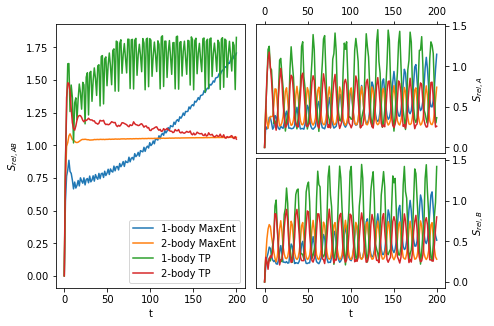
\includegraphics[scale = 0.7]{figs/section3_4/section5_bxb_low-closed_nonres/bxb_low_closed_nr_rel-entropy.png}
    \caption{En la presente figura mostramos la entropía relativa global $S_{rel,AB}$ (izquierda) y las entropías relativas parciales  $S_{rel,A}$ (derecha superior) y $S_{rel,B}$ (derecha inferior) \textit{vs.} tiempo para la evolución cerrada no resonante del estado \eqref{low_temp_state} para el sistema de dos bosones. Se han usado las dimensiones de \textit{cut-off} \texttt{dim1}= \texttt{dim2} = 10, frecuencias frecuencias $\omega_1 = 3.0$ y $\omega_2 =\sqrt{48}$ y un acoplamiento $\lambda = 0.05$ con $\beta=0.08$.}
    \label{low_temp_rel-entropy}
\end{figure}

Empezamos considerando un estado no gaussiano a una temperatura de forma tal que el número de ocupación bosónico del primer subsistema sea del orden de 5 estados. El estado a evolucionar será

\begin{equation}
    \rho_{AB}(0) = e^{-0.08{\bf a}^{\texttt{dim1}\dagger} {\bf a}^{\texttt{dim1}}} \otimes \mathds{1}_{\textnormal{\texttt{dim2}}}. \label{low_temp_state}
\end{equation}

Es claro que dicho estado está lejos de ser un estado gaussiano. Nos interesará estudiar que tan aplicables y confiables son los métodos aproximativos desarrollados anteriormente en describir esta dinámica. Se presentan los resultados a continuación junto con su análisis. 
En la figura \ref{low_temp_rel-entropy} se muestra la entropía relativa \textit{vs.} tiempo para el sistema global y para los subsistemas bosónicos.
Cómo podemos observar, los protocolos numéricos de un cuerpo \textcolor{blue}{ME1}, \textcolor{orange}{ME2} devuelven, a largo plazo, dinámicas virtualmente idénticas entre sí; estabilizándose entorno a un valor fijo de $2.0$ para la entropía global y entorno a $0.1$ para las entropías parciales para tiempos superiores a 150s.
Por otro lado, el protocolo \textcolor{red}{TP1} es inaplicable pero \textcolor{dark green}{TP2} es un formalismo aplicable, estabilizándose entorno a $0.5$ para tiempos mayores a 150s. Para las entropías relativas globales tenemos

\begin{gather*}
     \bigg|S(\rho_{\textnormal{\textcolor{blue}{ME1}}}|| \Tr_{1}\rho_{\textnormal{\textcolor{blue}{ME1}}} \otimes \Tr_{2}\rho_{\textnormal{\textcolor{blue}{ME1}}})(t) - S(\rho_{\textnormal{\textcolor{orange}{ME2}}}|| \Tr_{1}\rho_{\textnormal{\textcolor{orange}{ME2}}} \otimes \Tr_{2}\rho_{\textnormal{\textcolor{orange}{ME2}}})(t)  \bigg| \leq 1 \times 10^{-2}, \\ \bigg|S(\rho_{\textnormal{\textcolor{blue}{ME1}}}|| \Tr_{1}\rho_{\textnormal{\textcolor{blue}{ME1}}} \otimes \Tr_{2}\rho_{\textnormal{\textcolor{blue}{ME1}}})(t) -
     S(\rho_{\textnormal{\textcolor{dark green}{TP2}}}|| \Tr_{1}\rho_{\textnormal{\textcolor{dark green}{TP2}}} \otimes \Tr_{2}\rho_{\textnormal{\textcolor{dark green}{TP2}}})(t) \bigg| \leq 4.0.
\end{gather*}

\begin{figure}
\begin{minipage}{.5\linewidth}
\centering
\subfloat[]{\label{main:a}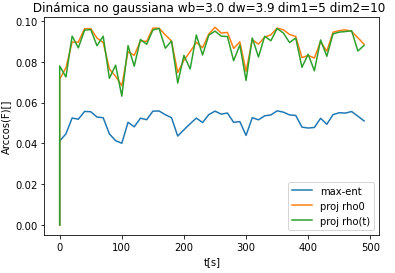
\includegraphics[scale=.71]{figs/section3_4/section5_bxb_low-closed_nonres/b5xb10_nonres_ng.png}}
\end{minipage}%
\begin{minipage}{.5\linewidth}
\centering
\subfloat[]{\label{main:b}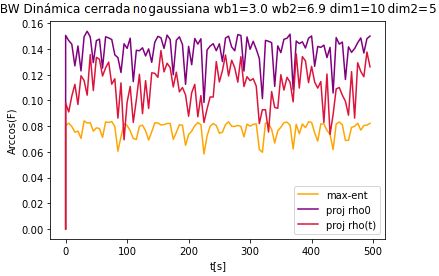
\includegraphics[scale=.7]{figs/section3_4/section5_bxb_low-closed_nonres/b10xb5_nonres_ng.png}}
\end{minipage}\par\medskip
\centering
\subfloat[]{\label{main:c}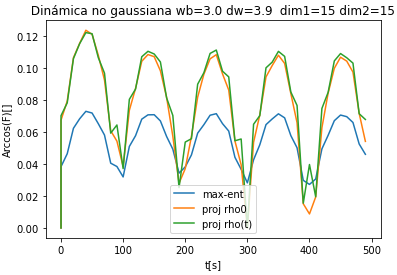
\includegraphics[scale=.75]{figs/section3_4/section5_bxb_low-closed_nonres/b15xb15_nonres_ng.png}}
\caption{Se muestran tres \textit{plots} de la métrica de Bures-Wooters \textit{vs.} tiempo para distintos pares de parámetros de truncamiento (\texttt{dim1},\texttt{dim2}): (5,10) mostrado en (a), (10,5) mostrado en (b) y (15,15) mostrado en (c), para la evolución cerrada no resonante del estado no gaussiano dado por \eqref{low_temp_state} con frecuencias $\omega_1 = 3.0$, $\omega_2 = \sqrt{48}$ y  constante de acoplamiento $\lambda = 0.05$. }
\label{closed_ng_nr}
\end{figure}

Pasamos a continuación a estudiar el comportamiento de la métrica de Bures-Wooters con el tiempo para los distintos protocolos. 
De los resultados presentados en la figura \ref{closed_ng_nr} observamos que las rutinas numéricas basadas en Proyección Ortogonal de dos cuerpos \textcolor{violet}{Proj rho0} y \textcolor{awesome}{Proj rho(t)} proveen virtualmente la misma dinámica, pues las curvas de Bures-Wooters asociadas tienen diferencias nunca superiores a $0.2$. Adicionalmente, para los casos de (\texttt{dim1},\texttt{dim2})=(5,10) y (\texttt{dim1},\texttt{dim2})=(10,5), la métrica de Bures calculada mediante dichas rutinas se estabilizan entorno a 0.08 y 0.05 respectivamente. Al aumentar los parámetros de truncamiento, notamos que las curvas obtenidas mediante Proyección Ortogonal empiezan a solaparse más con Max-Ent, lo cual es un excelente resultado; congruente con lo obtenido para la entropía relativa. Esto implica que el estado exacto del sistema puede ser aproximado por el estado Max-Ent de dos cuerpos o bien por alguno de los estados obtenidos por Proyección Ortogonal, sin que esto acarree un deterioro en la calidad de los resultados. 

Adicionalmente, en la figura \ref{ocupations_low_closed_nonres}
mostramos la evolución temporal de los operadores de ocupación de los subsistemas bosónicos ${\bf n}_1 = {\bf a}^{\texttt{dim1}\dagger} {\bf a}^{\texttt{dim1}}$, ${\bf n}_2 = {\mathbf b}^{\texttt{dim2}\dagger} {\mathbf b}^{\texttt{dim2}}$. De dichos gráficos podemos observar que la dinámica restringida de Max-Ent de uno y dos cuerpos, \textcolor{blue}{ME1} y \textcolor{orange}{ME2}, tienden a estabilizarse en torno al promedio de las oscilaciones, aproximadamente en $2.0$. Por otro lado, notamos que Proyección Ortogonal de uno y dos cuerpos, \textcolor{red}{TP1} y \textcolor{dark green}{TP2}, devuelven resultados similares entre sí para tiempos mayores a 125s, tendiendo a estabilizarse por debajo del mínimo de estas oscilaciones para ambos casos.

\begin{figure}
    \centering
    \subfloat[\centering ]{{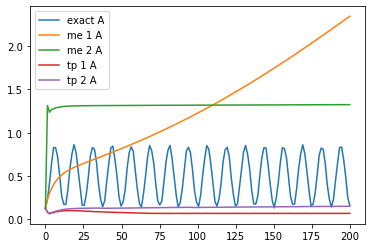
\includegraphics[scale=0.54]{figs/section3_4/section5_bxb_low-closed_nonres/bxb_low_closed_nr_n1.jpeg} }}
    \qquad
    \subfloat[\centering ]{{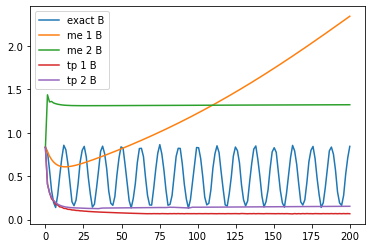
\includegraphics[scale=0.54]{figs/section3_4/section5_bxb_low-closed_nonres/bxb_low_closed_nr_n2.jpeg}}}
    \caption{En esta figura se presentan los resultados para la evolución del valor de expectación $\lgg {\bf n}_1 \rgg$ (izquierda) y la evolución del valor de expectación $\lgg {\bf n}_2 \rgg$ (derecha) con el tiempo para la evolución cerrada no resonante del estado no gaussiano  \eqref{low_temp_state}, para el sistema de dos bosones. Se han usado las dimensiones de \textit{cut-off} \texttt{dim1}= \texttt{dim2} = 10, con frecuencias $\omega_1 = 3.0$ y $\omega_2 =\sqrt{48}$ y un acoplamiento $\lambda = 0.05$.}
    \label{ocupations_low_closed_nonres}
\end{figure}

\begin{table}
     \caption{Comportamiento asintótico de las entropías relativas Dinámica Gaussiana cerrada no resonante}
     \begin{tabular}{llllll}
         \toprule
         & \( \textcolor{blue}{\textbf{Max-Ent 1}} \) & \( \textcolor{red}{\textbf{Proy. Ortg. 1}} \) & \( \textcolor{orange}{\textbf{Max-Ent 2}} \) & \( \textcolor{dark green}{\textbf{Proy. Ortg. 2}} \)  \\
        \midrule   \\
        $S(\rho_{\cdots}||\sigma)\xrightarrow[t\gg 200 {s}]{} $  & $1.9 \pm 0.1$, & N/A & $1.9 \pm 0.1$, & $5.0 \pm 0.1$.  \\
        $S(\rho_{\cdots_{A}}||\sigma_{A})\xrightarrow[t\gg 200 {s}]{} $ & $0.1 \pm 0.1$, & $5.0 \pm 0.01$ & $0.1 \pm 0.1$, & $2.0 \pm 0.01$ \\
        $S(\rho_{\cdots_{B}}||\sigma_{B})\xrightarrow[t\gg 200 {s}]{} $ & $0.5 \pm 0.4$, & N/A & $0.5 \pm 0.4$, & N/A. \\
        \bottomrule
        & \( \textcolor{orange}{\textbf{Max-Ent}} \) & \( \textcolor{violet}{\textbf{Proy. Ortg. 2 }} \rho_0 \) & \( \textcolor{awesome}{\textbf{Proy. Ortg. 2 }} \rho(t) \) \\
        ${\bf B}(\rho_{\cdots}, \sigma)\textnormal{  } \xrightarrow[t\gg 200 {s}]{}$ & $(9.0 \pm 0.1) \times 10^{-3}$, & $(1.25 \pm 0.32) \times 10^{-2}$, & $(1.20 \pm 0.30) \times 10^{-2}$, & {\small\textnormal{ para (\texttt{dim1}, \texttt{dim2}) = (5,10).}} \\
        & $(8.0 \pm 0.1) \times 10^{-2}$, & $0.13 \pm 0.1$, & $0.11 \pm 0.1$, & {\small\textnormal{ para (\texttt{dim1}, \texttt{dim2}) = (10,5).}}  \\
        & $0.25 \pm 0.20$ & $0.11 \pm 0.1$, & $0.11 \pm 0.1$, & {\small\textnormal{ para (\texttt{dim1}, \texttt{dim2}) = (15,15).}} \\
        \bottomrule
        & \( \textcolor{blue}{\textbf{Max-Ent 1}} \) & \( \textcolor{red}{\textbf{Proy. Ortg. 1}} \) & \( \textcolor{orange}{\textbf{Max-Ent 2}} \) & \( \textcolor{dark green}{\textbf{Proy. Ortg. 2}} \) \\
        $\lgg {\bf n}_1 \rgg\xrightarrow[t\gg 200 {s}]{}$ & $2.0 \pm 0.1$, & $ 0.10 \pm 0.01 $ & $2.0 \pm 0.1$, & $ 0.40 \pm 0.01 $.\\
        $\lgg {\bf n}_2 \rgg\xrightarrow[t\gg 200 {s}]{}$ & $2.5 \pm 0.2$, & $ 0.50 \pm 0.01 $ & $2.5 \pm 0.2$, & $ 0.50 \pm 0.01 $. \\
        \bottomrule
     \end{tabular} 
    \begin{tablenotes}
      \small
      \item En esta tabla presentamos los comportamientos asintóticos de las entropías relativas, de las métricas de Bures y los valores medios de los observables a tiempos largos para las rutinas implementadas. Los primeros tres resultados corresponden a aquellos de la figura \ref{low_temp_rel-entropy}, los siguientes tres corresponden a la figura \ref{closed_ng_nr} seguidos por aquellos mostrados en la figura \ref{ocupations_low_closed_nonres}. Los errores fueron calculados teniendo el cuenta el máximo de las oscilaciones. Los colores de las columnas están asociados a los colores de las curvas respectivas. 
    \end{tablenotes}
    \label{table4}
\end{table}

En la tabla \ref{table4} resumimos los resultados comentados anteriormente. 
Se concluye entonces que las rutinas numéricas implementadas, y sobre todo la dinámica de Proyección Ortogonal de dos cuerpos, son eficaces para la simulación de la dinámica exacta no resonante para el estado no gaussiano \eqref{low_temp_state} para el sistema de dos bosones.

\clearpage

\section{Sistema con acoplamiento bos\'on-esp\'in: Modelo de Dicke Simplificado}

En este capítulo estudiaremos un sistema de dos componentes: un subsistema bosónico y un subsistema de dos niveles con un acoplamiento bosón-espín, el \textbf{Modelo de Dicke simplificado}. Se estudiarán la dinámica cuasi gaussiana, donde la interacción conmuta con el Hamiltoniano espinorial, y una dinámica no gaussiana donde se elegirá una interacción donde esto no ocurre. \\

Este modelo físico consiste de dos componentes, un subsistema bosónico y un subsistema espinorial. En particular los estados del subsistema bosónico pertenecen al (completamiento del) espacio de Fock bosónico, a saber

\begin{align}
    \mathds{F}_{+}(\mathds{H}_b) = \overline{\bigoplus_{n=0}^{\infty} \textnormal{Sym}^{n} \mathds{H}_b^{\otimes n}} = \overline{\mathds{C} \oplus \mathds{H}_b \oplus (S_{+}(\mathds{H}_b \otimes \mathds{H}_b)) \oplus (S_{+}(\mathds{H}_b \otimes \mathds{H}_b \otimes \mathds{H}_b)) \oplus \cdots}.
\end{align}

donde nuevamente $\textnormal{Sym}^{n}$ es la simetrización del espacio de Hilbert de $n$ partículas, $\mathds{C}$ es el espacio de Hilbert asociado a un sistema sin partículas, $\mathds{H}_b$ es el espacio de Hilbert de un sistema con una única partícula, $S_{+}(\mathds{H}_b \otimes \mathds{H}_b)$ corresponde al espacio de Hilbert simetrizado del sistema con dos partículas y así sucesivamente. Los estados de Fock del sistema bosónico pueden ser construidos a partir de los operadores de creación y aniquilación bosónicos, a saber

$$
{\bf a}:\textnormal{Sym}^{N} \mathds{H} \rightarrow \textnormal{Sym}^{N-1} \mathds{H} \textnormal{ y }{\bf a}^{\dagger}: \textnormal{Sym}^{N}\mathds{H} \rightarrow \textnormal{Sym}^{N+1}\mathds{H}$$

que actúan sobre los estados de Fock de la forma usual.
En tales condiciones, el Hamiltoniano que rige a esta componente es ${\bf H}_b = \omega_a {\bf a}^{\dagger}{\bf a}$. \\

Un sistema de dos niveles es un sistema cuántico cuyo espacio de Hilbert es dos-dimensional $\mathds{H}_s \cong \mathds{C}^2$, dicho espacio se encuentra generado por un estado excitado $\ket{e}$ y un estado fundamental $\ket{g}$ con una diferencia $\Omega$ de energía entre ellos. Acorde a la mecánica cuántica, las partículas de espín $\frac{1}{2}$ son la representación fundamental del grupo $SU(2)$, siendo esta una representación unitaria irreducible, de dimensión $2\cdot \frac{1}{2} +1 =2$. Los estados de dicho espacio son construídos mediante los operadores 

\begin{align}
    \sigma_+ &= \ket{e}\bra{g} = \frac{1}{2} (\sigma_x + i\sigma_y),  & \sigma_- &= \ket{g}\bra{e} = \frac{1}{2} (\sigma_x - i\sigma_y), \\
    \sigma_+ & = \left( \begin{array}{cc}
       0 & 1 \\
       0 & 0
    \end{array} \right),  & \sigma_- & = \left( \begin{array}{cc}
       0 & 0 \\
       1 & 0
    \end{array} \right),
\end{align}

donde definimos las matrices de Pauli $\sigma_x, \sigma_y, \sigma_z$ como

\begin{align}
    \sigma_x &= \ket{e}\bra{g} + \ket{g}\bra{e}, & \sigma_y &= -i\ket{e}\bra{g} + i \ket{g}\bra{e} & \sigma_z &= \ket{e}\bra{e} - \ket{g}\bra{g}, \\
    \sigma_x & = \left( \begin{array}{cc}
       1 & 0 \\
       0 & 1
    \end{array} \right), & \sigma_y & = \left( \begin{array}{cc}
       0 & -i \\
       i & 0
    \end{array} \right), & \sigma_z & = \left( \begin{array}{cc}
       1 & 0 \\
       0 & -1
    \end{array} \right),
\end{align}

las cuales son los generadores de dicha representación irreducible dos-dimensional del grupo $SU(2)$ \cite{HoracioI}. Dichos generadores satisface el álgebra de Lie $\mathfrak{su(2)}$: $[\sigma_i,\sigma_j]={\bf i} \epsilon_{ijk}\sigma_k $, siendo $\epsilon_{ijk}$ el tensor de Levi-Civita completamente antisimétrico en tres índices. 
En este trabajo, nos interesará estudiar dos clases de Hamiltonianos espinoriales, a saber

\begin{align}
    {\bf H}_s^{(a)} = \frac{1}{2} \Omega \sigma_z \\
    {\bf H}_s^{(b)} = \frac{1}{2} \Omega \sigma_x,
\end{align}

donde esta elección de Hamiltonianos influirá en el tipo de dinámica a describir. Notemos que el modelo de Dicke posee una simetría global 
\begin{equation}
    \mathcal{P}: ({\bf a},\sigma^{\pm})\rightarrow (-{\bf a},-\sigma^{\pm}).
\end{equation}

Dicha simetría tiene dos autovalores: $1$ y $-1$, al actuar sobre los estados del sistema, a saber 

\begin{align}
    P & = (-1)^{{\bf N}_{ex}}, & {\bf N}_{ex} = {\bf a }^{\dagger}{\bf a} + \sigma_z,
\end{align}
donde $P$ es el número total de excitaciones. 

El Hamiltoniano que regirá la dinámica del sistema conjunto bosón-espín será escrito como la suma de los hamiltonianos bosónicos y espinoriales y un término de interacción adicional

\begin{equation}
    \mathbf{H}_D = \omega_a {\bf a}^{\dagger}{\bf a} + {\bf H}_s+ \lambda {\bf S}_z \frac{{\bf a}^{\dagger}+{\bf a}}{2},
    \label{model3.5_hamiltonian}
\end{equation}

donde el último término describe el acoplamiento entre el sistema de dos niveles y la cavidad con una magnitud $\lambda$ de acoplamiento\footnote{
Notemos que el último término de \eqref{model3.5_hamiltonian} puede ser escrito como la suma de dos términos: un término \textit{co-rotante} que conserva el número de excitaciones y es proporcional a ${\bf a}\sigma^{+} + {\bf a}^{\dagger}\sigma^{-}$ y un término \textit{contra-rotante} proporcional a ${\bf a}\sigma^{-} + {\bf a}^{\dagger}\sigma^{+}$, donde $\sigma^{\pm}=\sigma_{x}\pm {\bf i}\sigma_{y}$ son los operadores escalera de espín.}. \\

Siendo este un sistema bosón-espín un sistema no markoviano que presenta correlaciones e interacciones, podemos estudiarlo con los cuatro protocolos que hemos desarrollado en el presente trabajo de diploma: \textcolor{blue}{ME1}, \textcolor{orange}{ME2}, \textcolor{red}{TP1}, \textcolor{dark green}{TP2} y los casos particulares a este último protocolo, donde ponderamos con un estado fijo \textcolor{violet}{Proj rho0} y el protocolo donde ponderamos con un estado continuamente actualizado \textcolor{awesome}{Proj rho(t)}.
Ahora bien, para hacer los cálculos numéricos hemos de realizar un truncamiento del espacio de Hilbert bosónico a un número finito de estados, análogamente a como se realizaron estos cálculos en \autoref{two_boson_system}. En tal caso, los operadores de creación y aniquilación sobre cada modo bosónico son

\begin{subequations}
\begin{align}
{\bf a}_{i}\rightarrow {\bf a}^{N}_{i}=\sum_{n=0}^{N-1}\sqrt{n}|n\rangle_i \langle n+1|_i & \textnormal{ y }{\bf a}^{\dagger}_{i}\rightarrow {\bf a}^{\dagger N}_{i}=\sum_{n=0}^{N-1}\sqrt{n}|n+1\rangle_i \langle n|_i,
\end{align}
\end{subequations}

donde $N =$ \texttt{dim} $\mathds{H}$. En tales condiciones, estudiaremos

\begin{itemize}
    \item En la \autoref{dicke_gaussian}, se estudiará la evolución cuasi-gaussiana abierta no resonante y 
    \item en la \autoref{dicke_non-gaussian} se estudiará la evolución abierta no gaussiana no resonante para el sistema de Dicke simplificado,
\end{itemize}

buscando analizar la aplicabilidad de las rutinas desarrolladas en describir estas dinámicas. 

\subsection{Evolución gaussiana abierta no resonante}
\label{dicke_gaussian}

En la presente sección, estudiaremos la evolución gaussiana abierta no resonante del modelo de Dicke simplificado, donde la interacción conmuta con el Hamiltoniano espinorial, esto es consideramos el Hamiltoniano espinorial 

$$
{\bf H}_s^{(a)} = \frac{1}{2} \Omega \sigma_z.
$$

Acorde a la aproximación de onda rotante \cite{Nielsen.00}, el Hamiltoniano de interacción que resultará es

\begin{equation}
    \mathbf{H}_I = \lambda {\bf S}_z\frac{e^{{\bf i}\omega t}{\bf a}^{\dagger}+e^{-{\bf i}\omega t}{\bf a}}{2}.
    \label{model3.5_interaction}
\end{equation}

En tales condiciones, nos intereserá evolucionar un estado gaussiano, el cual puede ser escrito como

\begin{equation}
    \rho = e^{-\mathbf{K}}, \textnormal{ donde } \mathbf{K} = -(\mathbf{K}_{bos,1} \mathds{1}_2 + \mathbf{K}_{bos,2}\sigma_z) 
    \label{model3.5_rho}
\end{equation}

donde $\mathbf{K}_{bos,i}= \beta_{i}{\bf a}^{\dagger}{\bf a} + \psi_i,  \textnormal{ con } i =1,2$, donde $\sigma_{\mu}=(\mathds{1}_2, \boldsymbol{\sigma})$ es un "tetravector"  de las matrices de Pauli que incluye a la matriz identidad y donde todos los coeficientes son, \textit{a priori}, funciones $C^{1}(\mathds{R}_{+})$ en $t$. 

En un estudio \textit{ab initio} de este sistema, podemos realizar el cálculo analítico de la evolución cerrada del estado $\rho$, válida a cortos plazos. Para una evolución a cortos plazos $\delta t$, acorde al postulado \ref{Post time evolution} y al teorema de Stone sobre grupos unitarios fuertemente continuos de un parámetro, el operador de evolución unitaria sobre este sistema será $\mathcal{U} = e^{-i\delta t \mathbf{H}_I} \in \mathds{T}$, siendo $\mathds{T}$ el grupo unitario que tiene al hamiltoniano del sistema por generador. En consecuencia, 

\begin{equation}
    \rho = \exp (-\mathbf{K} - i\delta t [\mathbf{H}_I,\mathbf{K}] + \mathcal{O}((\delta t)^2) ).
\end{equation}

El resultado de dicha evolución será

\begin{equation}
    \rho(t) = \exp \bigg[ -\mathbf{K} -\lambda \left(\begin{array}{cc}
        \beta_2 (e^{-i\omega \delta t}{\bf a}-e^{i\omega \delta t}{\bf a}^{\dagger}) & \beta_2 (e^{-i\omega \delta t}{\bf a}-e^{i\omega \delta t}{\bf a}^{\dagger})  \\
        \beta_1 (e^{-i\omega \delta t}{\bf a}-e^{i\omega \delta t}{\bf a}^{\dagger}) & \beta_1 (e^{-i\omega \delta t}{\bf a}-e^{i\omega \delta t}{\bf a}^{\dagger}) 
    \end{array}\right) + \mathcal{O}((\delta t)^2)
    \bigg].
    \label{model3.4_rho1_ev}
\end{equation}

Mediante la ecuación de Liouville-von Neumann \eqref{Liouville eq}, hallamos que los coeficientes $\beta_i$, $\psi_i$, $i=1,2$ son independientes del tiempo y por tanto, sin pérdida de generalidad, pueden ser tomados como constantes arbitrarias fijas. Destaquemos que la validez de dicha aproximación está dada por la convergencia de la serie de Picard \cite{HeinzPetruccione}. Dicha evolución de un estado no gaussiano inicialmente descorrelacionado, devuelve un estado no gaussiano con correlaciones de pares; demostrando esto que este sistema es no markoviano. Esto demuestra que la evolución de una dinámica, cerrada o abierta, dependerá exclusivamente de la conmutatividad o no de la interacción bosón-espín y del Hamiltoniano espinorial. \\

Para los cálculos numéricos, se tomó un parámetro de truncamiento inicial de \texttt{dim}=10, operadores de colapso bosónicos con factores de colapso $\gamma_1 = 0.05$, $\gamma_2 = 0.1$ y frecuencias $\omega_1 = 3$,  $\omega_2 = \sqrt{48}$ y  constante de acoplamiento $\lambda = 0.05$. Se toma el estado inicial gaussiano descorrelacionado dado por \eqref{model3.5_rho}.

\begin{figure}
    \centering
    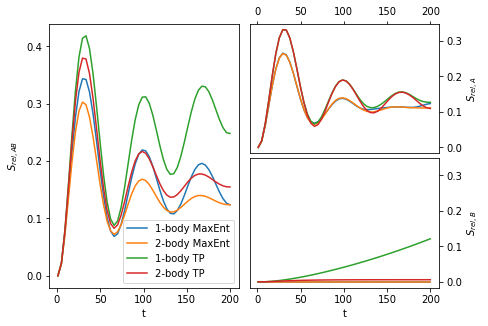
\includegraphics[scale=0.7]{figs/section3_4/section5_bxs-open-nonres/rel_entropy_bxs_nonres.png}
    \caption{En la presente figura mostramos la entropía relativa global $S_{rel,AB}$ para la evolución cerrada no resonante de un estado gaussiano para el sistema de Dicke simplificado. Se tomó un parámetro de truncamiento de \texttt{dim}=10, operadores de colapso bosónicos con factores de colapso $\gamma_1 = 0.05$, $\gamma_2 = 0.1$ y frecuencias $\omega_1 = 3$, $\omega_2 = \sqrt{48}$ y  constante de acoplamiento $\lambda = 0.05$.}
    \label{rel_entropy_open_nonres.png}
\end{figure}

En la figura \ref{rel_entropy_open_nonres.png} se muestra la entropía relativa \textit{vs.} tiempo para los distintos protocolos implementados. De estos resultados observamos que las dinámicas de dos cuerpos, \textcolor{orange}{ME2} y \textcolor{dark green}{TP2}, devuelven virtualmente la misma dinámica, no divergente a largos plazos. Esta tiende a estabilizarse entorno a $8 \times 10^{-5}$. Por otro lado, si bien las rutinas de un cuerpo  \textcolor{blue}{ME1}, \textcolor{red}{TP1} tienen una tendencia creciente, crecen muy lentamente (notar la escala) por lo que a largos plazos siguen siendo aplicables. 

Luego, los estados calculados mediantes estas rutinas son poco distinguibles del estado exacto, por lo que nos interesa cuantificar esta diferencia (en el sentido geométrico) mediante la métrica de Bures-Wooters acorde a la dinámica restringida Max-Ent de dos cuerpos \textcolor{orange}{ME2} y acorde a la proyección ortogonal de dos cuerpos ponderada por un estado fijo y por un estado continuamente actualizado, \textcolor{violet}{Proj rho0} y \textcolor{awesome}{Proj rho(t)} respectivamente. Dichos resultados se muestran en la figura 
\ref{bxb-closed-res/bxb_open_nr.png}. 

\begin{figure}
\begin{minipage}{.5\linewidth}
\centering
\subfloat[]{\label{main:a}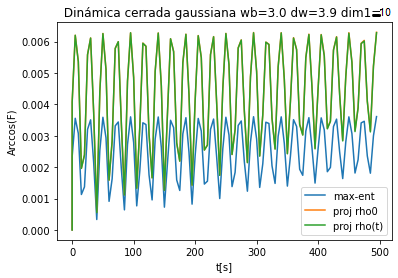
\includegraphics[scale=.57]{figs/section3_4/section5_bxs-open-nonres/b10xs_nonres_g.png}}
\end{minipage}%
\begin{minipage}{.5\linewidth}
\centering
\subfloat[]{\label{main:b}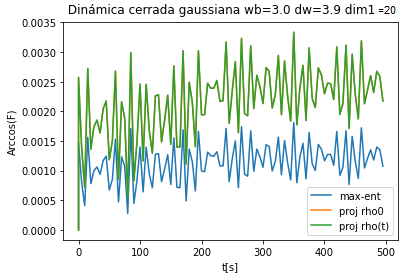
\includegraphics[scale=.57]{figs/section3_4/section5_bxs-open-nonres/b20xs_nonres_g.png}}
\end{minipage}\par\medskip
\centering
\subfloat[]{\label{main:c}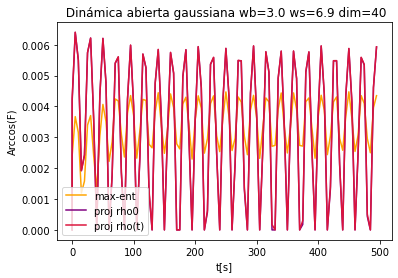
\includegraphics[scale=.65]{figs/section3_4/section5_bxs-open-nonres/b40xs_nonres_g.png}}
\caption{Se muestran tres \textit{plots} de la métrica de Bures-Wooters \textit{vs.} tiempo para distintos pares de parámetros de truncamiento para la evolución cerrada no resonante del estado cuasi gaussiano dado por \eqref{model3.6_gaussian1}. Se tomó un parámetro de truncamiento de dim=10, operadores de colapso bosónicos con factores de colapso $\gamma_1 = 0.05$, $\gamma_2 = 0.1$ y frecuencias $\omega_1 = 3$ y $\omega_2 = \sqrt{48}$ y constante de acoplamiento $\lambda = 0.05$. Se estudiaron los casos de \texttt{dim} = 10 mostrado en (a), 20 mostrado en (b) y 40 mostrado en (c). }
\label{bxb-closed-res/bxs_open_nr.png}
\end{figure}

En primera instancia, notamos que las curvas obtenidas por ambas variantes de Proyección Ortogonal son idénticas. La diferencia entre dichas es imperceptible en la escala de los gráficos, siendo de tan solo $5 \times 10^{-4}$. Por otro lado, dichas son también virtualmente idénticas a la curva obtenida para Max-Ent, con una diferencia nunca mayor a $0.03$ para los primeros dos casos de truncamiento. Los resultados son prometedores y se condicen con aquellos obtenidos para la entropía relativa en \ref{rel_entropy_open_nonres.png}.

\begin{figure}
    \centering
    \subfloat[\centering ]{{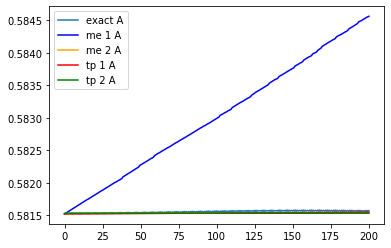
\includegraphics[scale=0.57]{figs/section3_4/section5_bxs-open-nonres/expectation_value_n1_bxs_nonres.png}}}
    \qquad
    \subfloat[\centering ]{{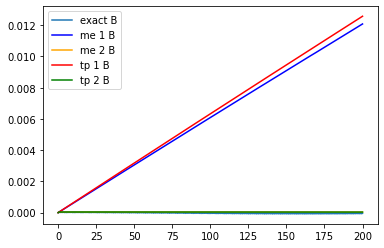
\includegraphics[scale=0.57]{figs/section3_4/section5_bxs-open-nonres/expectation_value_n2_bxs_nonres.png}}}
    \caption{En esta figura se presentan los resultados para la evolución del valor de expectación $\lgg { \bf n}_1 \rgg$ (figura de la izquierda) y la evolución del valor de expectación $\lgg { \bf S}_z \rgg$ (figura de la derecha) con el tiempo para la evolución cerrada resonante de un estado gaussiano para el sistema de Dicke simplificado. Se tomó un parámetro de truncamiento de \texttt{dim}=10, operadores de colapso bosónicos con factores de colapso $\gamma_1 = 0.05$, $\gamma_2 = 0.1$ y frecuencias $\omega_1 = 3$ y $\omega_2 = \sqrt{48}$ y una constante de acoplamiento $\lambda = 0.05$.}
    \label{ocupations_open_res}
\end{figure}

Finalmente, en la figura \ref{ocupations_open_res}, se presentan los resultados para la evolución del valor de expectación $\lgg {\bf n}_1 \rgg$ y la evolución del valor de expectación $\lgg {\bf S}_z \rgg$. Notamos que, pese a la gran similitud entre la eficacia de Max-Ent y Proyección Ortogonal, las rutinas de Proyección ortogonal aún son incapaces de modelar correctamente la dependencia temporal exacta de estos operadores, por lo que se deberán de corregir en futuros estudios.

\begin{table}
     \caption{Comportamiento asintótico de las entropías relativas Dinámica Gaussiana cerrada no resonante}
     \begin{tabular}{llllll}
        \toprule
         & \( \textcolor{blue}{\textbf{Max-Ent 1}} \) & \( \textcolor{dark green}{\textbf{Proy. Ortg. 1}} \) & \( \textcolor{orange}{\textbf{Max-Ent 2}} \) & \( \textcolor{red}{\textbf{Proy. Ortg. 2}} \)  \\
        \midrule   \\
        $S(\rho_{\cdots}||\sigma)\xrightarrow[t\rightarrow\infty]{} $  & $0.15 \pm 0.5$ & $\infty$ & $0.12 \pm 0.01$ & $0.14 \pm 0.1$   \\
        $S(\rho_{\cdots_{A}}||\sigma_{A})\xrightarrow[t\rightarrow\infty]{} $ & $0.10 \pm 0.05$ & $0.10 \pm 0.05$ & $0.10 \pm 0.05$ & $0.10 \pm 0.05$ \\
        $S(\rho_{\cdots_{B}}||\sigma_{B})\xrightarrow[t\rightarrow\infty]{}$ & $0.01 \pm 0.01$ & $\infty$ & $0.01 \pm 0.01$ & $0.01 \pm 0.01$ \\
        \bottomrule
        & \( \textcolor{orange}{\textbf{Max-Ent}} \) & \( \textcolor{violet}{\textbf{Proy. Ortg. 2 }} \rho_0 \) & \( \textcolor{awesome}{\textbf{Proy. Ortg. 2 }} \rho(t) \) \\
        ${\bf B}(\rho_{\cdots}, \sigma)\textnormal{  } \xrightarrow[t\gg 200 {s}]{}$ & $(2 \pm 1)\times 10^{-3}$, & $(4 \pm 2)\times 10^{-3}$, &$(4 \pm 2)\times 10^{-3}$ , & {\small\textnormal{ para \texttt{dim}=10.}} \\
        &$(2.5 \pm 0.5)\times 10^{-3}$,& $(3 \pm 3)\times 10^{-3}$,& $(3 \pm 3)\times 10^{-3}$, & {\small\textnormal{ para \texttt{dim}=20.}}  \\
        &$(2.5 \pm 0.5)\times 10^{-3}$,& $(3 \pm 3)\times 10^{-3}$,& $(3 \pm 3)\times 10^{-3}$, & {\small\textnormal{ para \texttt{dim}=40.}} \\
        \bottomrule
        & \( \textcolor{orange}{\textbf{Max-Ent 1}} \) & \( \textcolor{red}{\textbf{Proy. Ortg. 1}} \) & \( \textcolor{dark green}{\textbf{Max-Ent 2}} \) & \( \textcolor{violet}{\textbf{Proy. Ortg. 2}} \) \\
        $\lgg {\bf n} \rgg\xrightarrow[t\rightarrow\infty]{}$ & $\infty$ & $ 0.04 \pm 0.01 $ & $0.90 \pm 0.01$ & $(4.5 \pm 0.5) \times 10^{-3}$.\\
        $\lgg {\bf S}_z \rgg\xrightarrow[t\rightarrow\infty]{}$ & $\infty$ & $\infty$ & $0.10 \pm 0.01$ & $ 0.0 \pm 0.0$. \\
        \bottomrule
     \end{tabular} 
    \begin{tablenotes}
      \small
      \item En esta tabla presentamos los comportamientos asintóticos de las entropías relativas, de las métricas de Bures y los valores medios de los observables a tiempos largos para las rutinas implementadas. Los primeros tres resultados corresponden a aquellos de la figura \ref{rel_entropy_open_nonres.png}, los siguientes tres corresponden a la figura \ref{bxb-closed-res/bxs_open_nr.png} seguidos por aquellos mostrados en la figura \ref{ocupations_open_res}. Los errores fueron calculados teniendo el cuenta el máximo de las oscilaciones. Los colores de las columnas están asociados a los colores de las curvas respectivas. 
    \end{tablenotes}
    \label{table4}
\end{table}

Concluimos que Proyección Ortogonal es un formalismo muy útil para describir esta evolución para el modelo de Dicke simplificado. 

\subsection{Evoluci\'on no gaussiana para un sistema con acoplamiento bos\'on-esp\'in}
\label{dicke_non-gaussian}

En esta sección, estudiaremos la evolución abierta no gaussiana no resonante para el sistema de Dicke simplificado, tomando un hamiltoniano de interacción bosón-espín que no conmute con el Hamiltoniano espinorial.

En este caso tomaremos al Hamiltoniano espinorial como ${\bf H}_s = \frac{1}{2}\Omega\sigma_x$ con la base de operadores de espín dada por todas las matrices de Pauli y la identidad. Es decir, que ahora los operadores de espín que actúan sobre este sistema son $\{\mathbf{1}_2, \sigma_x, \sigma_y, \sigma_z\}$. Dado que la interacción no conmuta con el Hamiltoniano espinorial, la evolución será no gaussiana. Tomaremos un estado inicial

\begin{equation}
    \rho_{ng}= e^{-\mathbf{K}_{ng}}, \textnormal { donde } \mathbf{K}_{ng} = \sum_{\mu=0}^{4} \bigg(\alpha_{\mu}(t){\bf a}^{\dagger}{\bf a}{\bf +} \zeta_{\mu}{\bf a} + \zeta_{\mu}^{*}{\bf a}^{\dagger} + \phi_{\mu}\bigg) \sigma_{\mu},
    \label{model3.7_rho}
\end{equation}

donde los parámetros $\alpha_{\mu},  \zeta_{\mu}$ y $\phi_{\mu} \in \mathds{C}$ y donde $\sigma_{\mu} = (\mathds{1}_2, {\boldsymbol \sigma})$ son los operadores en la base espinorial. 

Debido a la complejidad de dichos cálculos, no disponemos de una expresión analítica de dicha evolución debiendo usar los distintos protocolos y métodos numéricos explicados anteriormente. Sin embargo, sabemos que el estado evolucionado continuará siendo no gaussiano; admitiendo una descomposición no unívoca

$$
\mathbf{K}_{ng}(t) = -\log \rho_{ng}(t) = \mathbf{K}_{g}(t)+\mathbf{K}_{r}(t),
$$

es decir, una parte gaussiana y otra no gaussiana residual. Nos interesa saber el cambio que ha sufrido $\mathbf{K}_{r}$, si ha aumentado o disminuido respecto al punto de partida inicial. 

\begin{figure}
    \centering
    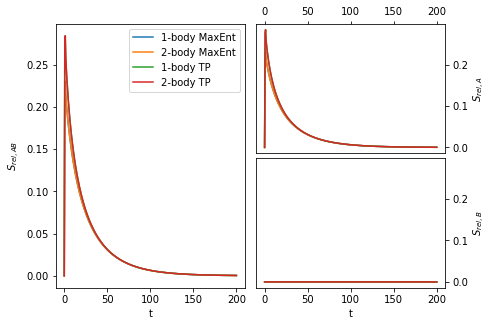
\includegraphics[scale=0.7]{figs/section3_4/section5_bxs_ng/rel_entropy_open_nonres_ng.png}
    \caption{En la presente figura mostramos la entropía relativa $S_{rel,AB}$ (izquierda) y las entropías parciales $S_{rel,A}$ (derecha superior) y $S_{rel,B}$ (derecha inferior) \textit{vs.} tiempo para la evolución abierta resonante de un estado no gaussiano para el modelo de Dicke simplificado, usando operadores de colapso bosónicos. Se ha usado las dimensiones de \textit{cut-off} \texttt{dim}=10, frecuencias $\omega_1 = 3.0$, $\omega_2 = 6.08$ y factores de colapso $\gamma_1 = 0.1$, $\gamma_2 = 2 \gamma_1$ con un acoplamiento $\lambda= 0.05$}
    \label{rels_open-nr}
\end{figure}

\begin{figure}
    \centering
    \subfloat[\centering ]{{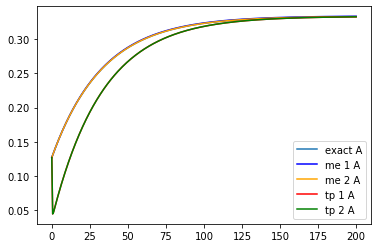
\includegraphics[scale=0.55]{figs/section3_4/section5_bxs_ng/n1_ocupation_number_open_nonres_ng.png} }}
    \qquad
    \subfloat[\centering]{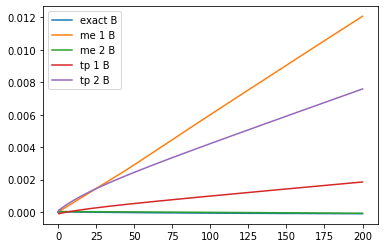
\includegraphics[scale=0.55]{figs/section3_4/section5_bxs_ng/sigmaz_open_nonres_ng.png}}
    \caption{En esta figura se muestran la evolución temporal del valor de expectación del operador número bosónico $\langle {\bf n} \rangle $ (izquierda) y el valor de expectación del operador $\langle {\bf S}_z \rangle$ (derecha). Se han usado  frecuencias $\omega_1 = 3$ y $\omega_2 = 6.08$, parámetros de colapso $\gamma_1 = 0.01$, $\gamma_2 = 0.02$ y acoplamiento $\lambda = 0.05$.}
    \label{results_open-nr}
\end{figure}

En la figura \ref{rels_open-nr} mostramos la entropía relativa global al sistema $S_{AB}$ \textit{vs.} tiempo para esta evolución. Notamos que no hay diferencia significativa entre protocolos y los cuatros protocolos \textcolor{blue}{ME1}, \textcolor{orange}{ME2}, \textcolor{red}{TP1}, \textcolor{dark green}{TP2} devuelven los mismos resultados. Buscamos entónces cuantificar esta diferencia entre estados aproximados y estado exacto mediante la métrica de Bures-Wooters. En la figura \ref{dicke_ng} mostramos los \textit{plots} de la dependencia temporal de la métrica de Bures-Wooters para los tres protocolos usados, para distintas dimensiones del espacio de Hilbert bosónico.

\begin{figure}
\begin{minipage}{.5\linewidth}
\centering
\subfloat[]{\label{main:a}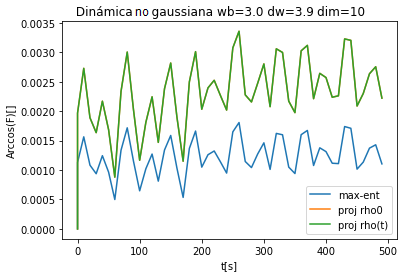
\includegraphics[scale=.75]{figs/section3_4/section5_bxs_ng/b10xs_nonres_ng.png}}
\end{minipage}%
\begin{minipage}{.5\linewidth}
\centering
\subfloat[]{\label{main:b}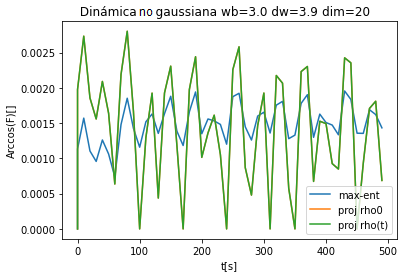
\includegraphics[scale=.75]{figs/section3_4/section5_bxs_ng/b20xs_nonres_ng.png}}
\end{minipage}\par\medskip
\centering
\subfloat[]{\label{main:c}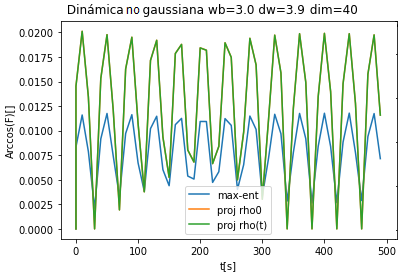
\includegraphics[scale=.75]{figs/section3_4/section5_bxs_ng/b40xs_nonres_ng.png}}
\caption{Se muestran tres \textit{plots} de la métrica de Bures-Wooters \textit{vs.} tiempo para distintos pares de parámetros de truncamiento para la evolución cerrada no resonante del estado no gaussiano dado por \eqref{dicke_non-gaussian}. Se estudiaron los pares de \texttt{dim}: 10 - figura (a) -, 20 - figura (b) - y 40 - figura (c) -. Se usan los operadores de colapso ${\bf C}_1 = {\bf a}^{\texttt{dim}}$ y ${\bf C}_2 = {\bf a}^{\texttt{dim}\dagger}$ con factores de colapso $\gamma_1 = 0.05$, $\gamma_2 = 0.1$ y frecuencias $\omega_1 = 3$ y $\omega_2 = 6.08$ y una constante de acoplamiento $\lambda = 0.05$.}
\label{dicke_ng}
\end{figure}

Notamos que en los tres plots mostrados, no hay diferencias significativas entre protocolos, siendo esto un excelente resultado. La diferencia entre los protocolos de Proyección Ortogonal, es virtualmente nula siendo aproximadamente de $5\times 10^{-4}$. Por otro lado, la diferencia entre Proyección Ortogonal y Max-Ent nunca es superior a $5\times 10^{-4}$. Nuevamente, recordemos que Proyección Ortogonal de dos cuerpos es computacionalmente menos costoso que Max-Ent de dos Cuerpos por lo que esto implica que el estado exacto puede ser aproximado por aquel calculado mediante Proyección Ortogonal sin tener que usar Max-Ent y sin incurrir en un deterioro consiguiente en la calidad de resultados. Estos resultados se condicen con aquellos obtenidos para la entropía relativa en la figura \ref{rels_open-nr}. 

Por otro lado, en \ref{results_open-nr} se muestran las evoluciones temporal del valor de expectación del operador número bosónico $\langle {\bf n} \rangle $ y el valor de expectación del operador $\langle {\bf S}_z \rangle$. De dichos resultados observamos que las cuatro rutinas son eficientes en la simulación de la dinámica exacta en lo que respecta al cálculo de la evolución temporal del valor de expectación del primer operador. 
Del segundo gráfico, observamos que las rutinas de Proyección Ortogonal de uno y dos cuerpos y  Max-Ent de un cuerpo no describen correctamente la dinámica exacta para el segundo caso.\\

\begin{table}
     \caption{Comportamiento asintótico de las entropías relativas Dinámica Gaussiana cerrada no resonante}
     \begin{tabular}{llllll}
        \toprule
         & \( \textcolor{blue}{\textbf{Max-Ent 1}} \) & \( \textcolor{dark green}{\textbf{Proy. Ortg. 1}} \) & \( \textcolor{orange}{\textbf{Max-Ent 2}} \) & \( \textcolor{red}{\textbf{Proy. Ortg. 2}} \)  \\
        \midrule   \\
        $S(\rho_{\cdots}||\sigma)\xrightarrow[t\rightarrow\infty]{} $  & $0.0 \pm 0.0$ &  $0.0 \pm 0.0$ &  $0.0 \pm 0.0$ &  $0.0 \pm 0.0$   \\
        $S(\rho_{\cdots_{A}}||\sigma_{A})\xrightarrow[t\rightarrow\infty]{} $ & $0.0 \pm 0.0$ &  $0.0 \pm 0.0$ &  $0.0 \pm 0.0$ &  $0.0 \pm 0.0$ \\
        $S(\rho_{\cdots_{B}}||\sigma_{B})\xrightarrow[t\rightarrow\infty]{}$ & $0.0 \pm 0.0$ &  $0.0 \pm 0.0$ &  $0.0 \pm 0.0$ &  $0.0 \pm 0.0$ \\
        \bottomrule
        & \( \textcolor{orange}{\textbf{Max-Ent 1}} \) & \( \textcolor{red}{\textbf{Proy. Ortg. 1}} \) & \( \textcolor{dark green}{\textbf{Max-Ent 2}} \) & \( \textcolor{violet}{\textbf{Proy. Ortg. 2}} \) \\
        $\lgg {\bf n} \rgg\xrightarrow[t\rightarrow\infty]{}$ & $\infty$ & $ 0.35 \pm 0.01 $ & $ 0.35 \pm 0.01 $ & $ 0.35 \pm 0.01 $.\\
        $\lgg {\bf S}_z \rgg\xrightarrow[t\rightarrow\infty]{}$ & $\infty$ & $\infty$ & $0.0 \pm 0.0$ & $\infty$. \\
        \bottomrule
        & \( \textcolor{orange}{\textbf{Max-Ent}} \) & \( \textcolor{violet}{\textbf{Proy. Ortg. 2 }} \rho_0 \) & \( \textcolor{awesome}{\textbf{Proy. Ortg. 2 }} \rho(t) \) \\
        ${\bf B}(\rho_{\cdots}, \sigma)\textnormal{  } \xrightarrow[t\gg 200 {s}]{}$ & $(1.0 \pm 0.5) \times 10^{-3}$, & $(2.5 \pm 0.5) \times 10^{-3}$, & $(2.5 \pm 0.5) \times 10^{-3}$, & {\small\textnormal{ para \texttt{dim}=10.}} \\
        &$(1.2 \pm 0.5) \times 10^{-3}$,& $(1.2 \pm 1.0) \times 10^{-3}$, & $(1.2 \pm 1.0) \times 10^{-3}$, & {\small\textnormal{ para \texttt{dim}=20.}}  \\
        &$(2.5 \pm 0.5) \times 10^{-3}$,& $0$,& $0$, & {\small\textnormal{ para \texttt{dim}=40.}} \\
     \end{tabular} 
    \begin{tablenotes}
      \small
      \item En esta tabla presentamos los comportamientos asintóticos de las entropías relativas, de las métricas de Bures y los valores medios de los observables a tiempos largos para las rutinas implementadas. Los primeros tres resultados corresponden a aquellos de la figura \ref{rels_open-nr}, los siguientes dos corresponden a la figura \ref{dicke_ng} seguidos por aquellos mostrados en la figura \ref{results_open-nr}. Los errores fueron calculados teniendo el cuenta el máximo de las oscilaciones. Los colores de las columnas están asociados a los colores de las curvas respectivas. 
    \end{tablenotes}
    \label{table4}
\end{table}

No obstante, concluimos entonces que el protocolo de Proyección Ortogonal de dos cuerpos es un excelente formalismo útil en la descripción de este sistema no markoviano, tanto en dinámicas gaussianas como no gaussianas.

\clearpage

\chapter{Conclusiones y futuros desarrollos}
\label{Chapter6}

En el presente trabajo hemos estudiado los resultados analíticos de las evoluciones cerradas y abiertas de estados gaussianos y no gaussianos para diversos sistemas, un modelo de dos subsistemas bosónicos acoplados y un sistema con un acoplamiento espín-bosón mediante el uso de diversas aproximaciones markovianas y no markovianas.

En el  \autoref{cap3_dosbosones} estudiamos, en primera instancia, la solución analítica de la dinámica cerrada de un sistema de dos bosones mediante la diagonalización de su hamiltoniano. A continuación, en la  \autoref{chap3_dingauss}, se utilizó el formalismo de dinámicas gaussianas para estudiar la evolución cerrada de dicho sistema comparando estos resultados con aquellos obtenidos numéricamente. Se encuentra que el formalismo de dinámicas gaussianas devuelve resultados fidedignos y es un formalismo adecuado para tratar nuestro modelo, en el régimen de bajas temperaturas y correlaciones pequeñas. Luego, en la  \autoref{sec3_3TratamientoApproximado}, se estudió la evolución de un estado reducido de un subsistema bosónico sin conocer información sobre su entorno, haciendo uso de la aproximación Markoviana y del formalismo provisto por la ecuación de Lindblad. Se compararon dichos resultados con aquellos obtenidos numéricamente encontrando discrepancias significativas en el comportamiento del sistema. Esto se debe precisamente a que el sistema de dos bosones es un sistema no markoviano, siendo la ecuación de Lindblad un formalismo inadecuado para su descripción. 

En el \autoref{chap4_allmaxent} se introdujo el principio Max-Ent y el enfoque de gaussianización como aplicación del Principio Max-Ent como un formalismo útil para la descripción de sistemas no markovianos. Se plantean los fundamentos de las dinámicas Max-Ent restringidas de uno y dos cuerpos en base a un proceso de optimización de parámetros de un estado de Gibbs. Siendo este proceso de optimización un procedimiento computacionalmente costoso, también se derivó un formalismo de Proyección ortogonal de uno y dos cuerpos basado en la minimización de una distancia entre estados. 

En el \autoref{chapter5} se estudiaron las aplicaciones de las rutinas numéricas implementadas anteriormente, buscando analizar su efectividad en la descripción de las evoluciones de dos tipos de sistemas.

Para el sistema de dos bosones se estudiaron diversas dinámicas cuasi-gaussianas y no gaussianas, a saber: una dinámica cerrada no resonante cuasi-gaussiana en la \autoref{bxb_c_nr_g}, una dinámica cerrada cuasi-gaussiana resonante en la \autoref{bxb_cr}, una dinámica abierta cuasi-gaussiana no resonante en la 
\autoref{bxb_or} y una dinámica no gaussiana cerrada no resonante en la
\autoref{bxb_cnr}. Para el modelo de Dicke, se buscó analizar la efectividad de las rutinas numéricas implementadas en la descripción de una dinámica gaussian abierta no resonante en \autoref{dicke_gaussian} y también se buscó estudiar la viabilidad de modelar dinámica no gaussianas. Estas son obtenidas de una no conmutatividad del Hamiltoniano espinoral con la interacción y fueron estudiadas en  \autoref{dicke_non-gaussian}.

Para el sistema de dos bosones, en general, se obtuvo que los formalismos implementados devuelven resultados fidedignos a la dinámica exacta, presentando algunos inconvenientes en algunos casos particulares que ya han sido discutidos en cada sección. Estos resultados implican que se puede aproximar el estado exacto del sistema mediante los estados obtenidos mediante dichas rutinas sin incurrir en un deterioro significativo de la calidad de los resultados respecto a los exactos. Además esto implica que las dinámicas modeladas, lejanas a la condición de gaussianidad exacta, no están regidas por correlaciones de orden mayor a las estudiadas, al menos a largo plazo. Vale destacar que las dinámicas resonantes resultan, en general, más difíciles de modelar puesto que incluso teoría de perturbaciones es inaplicable para acoplamientos débiles.

Sin embargo, estos son resultados alentadores que demuestran un buen grado de aplicabilidad del formalismo de Proyección Ortogonal, el cual es menos costoso en recursos computacionales que su contraparte Max-Ent de dos cuerpo,s en la descripción de sistemas no markovianos. En el futuro, se plantea estudiar y corregir las rutinas numéricas de forma tal de mejorar los resultados.

Por otro lado, para el sistema de Dicke simplificado, se obtuvo en general, excelente acuerdo entre los resultados exactos y aquellos obtenidos mediante Proyección Ortogonal de dos cuerpos y Max-Ent de dos cuerpos, lo cual afianza nuestra conclusión enunciada anteriormente. 

En futuros desarrollos, buscaremos aplicar el formalismo Max-Ent y de Proyección Ortogonal para modelar la dinámica de sistemas de espines con interacciones de corto alcance, fermiones en una red y gases de bosones y generalizar este formalismo para  sistemas fuertemente correlacionados y sistemas que involucren dinámicas no markovianas.

\appendix

\chapter{Algunos Aspectos Técnicos de Teoría de la Informaci\'on Cu\'antica}
\label{Appendix A}
\section{El Operador Densidad}

En el \autoref{chapter2} se formularon los axiomas de la teoría de la información cuántica en términos de un operador densidad $\rho$ definido en un ensamble y no de los vectores del espacio de Hilbert corrugado. El objetivo de este apéndice es motivar esta reformulación de la mecánica cuántica y profundizar en los conceptos de estados puros, mixtos y estados entrelazados y separables, concluyendo con algunas consideraciones propias de topología algebraica.  

Consideramos un experimento en el cual una fuente emite un haz de átomos, no es posible conocer los estados individuales de cada átomo; luego la información sobre el sistema es \textit{incompleta}. Lo que se puede asegurar es que el estado del sistema está en el ensamble  $\{p_k, \ket{\psi_k}\}_{k=1}^{n}$ ie. el estado del sistema es un \textbf{estado mixto} mientras que los estados individuales $\ket{\psi_k}$ son \textbf{estados puros} \cite{B.C.G.STR, Nielsen.00}. \footnote{Es importante destacar que el estado mixto no es el mismo concepto que la superposición de estados $\ket{\psi} = \sum_{k} c_k \ket{\psi_k}$ con $|c_k|^2 = p_k$. Se puede demostrar que es imposible describir un estado mixto mediante un vector promedio en dicho espacio de Hilbert pero sí puede ser descrito mediante el operador densidad.}

Luego, dado un observable ${\bf A}$, la probabilidad $p(i)$ de obtener el resultado $a_i$ en una medida sobre dicho sistema es:

$$
p(i) = \sum_{k=1}^{l} p_k \bra{\psi_k}\mathbf{P}_i \ket{\psi_k}
$$

siendo ${\bf P}_i$ el proyector sobre el subespacio asociado con el autovalor $a_i$ de ${\bf A}$. Luego, el valor esperado del observable es

$$
\langle A \rangle = \sum_{i = 1}^{n} a_i p(i) = \sum_{k=1}^{l} p_k \sum_{i=1}^{n} a_i \bra{\psi_k}\mathbf{P}_i\ket{\psi_k} = \sum_{k=1}^{l} p_k \bra{\psi_k}\mathbf{A}\ket{\psi_k}.
$$

Luego la teoría de la probabilidad surge naturalmente en dos instancias

\begin{itemize}
    \item en el desconocimiento inicial de la información sistema, al dar los pesos iniciales $p_k$ de los estados del ensamble
    \item y en el procedimiento de medida, caracterizado por las probabilidades $ \bra{\psi_k}\mathbf{P}_i \ket{\psi_k}$ de obtener los resultados $a_i$ en la medida de un observable ${\bf A}$ cuando el sistema se encuentra en el estado $\ket{\psi_k}$. 
\end{itemize}

\break

Para poder tener en cuenta ambos factores, la información parcial sobre el sistema y la naturaleza probabilistíca de la mecánica cuántica, es útil construir el operador densidad 

$$
\rho = \sum_{k} p_k \ket{\psi_k}\bra{\psi_k},
$$

el cual caracterizará completamente al estado del sistema, acorde al Postulado \ref{Post state space}. Las medidas pueden ser escritas acorde al Postulado \ref{Post measurement} y su evolución temporal está dada por el Postulado \ref{Post time evolution}. Esta reformulación de la teoría cuántica se debe a que los estados densidad, construidos respecto a un ensamble, proveen de la descripción correcta para sistemas compuestos en los cuales los estados de los subsistemas pueden no ser totalmente conocidos. Adicionalmente, la formulación de matrices densidad describe correctamente el entrelazamiento cuántico, donde es posible que el estado global al sistema sea un estado puro pero que los estados individuales sean mixtos. 

%Resulta que los estados cumplen que $\Tr \rho^2 \leq 1$, donde la igualdad estricta se cumple únicamente para estados puros mientras que para estados mixtos vale la desigualdad estricta. 

\begin{figure}
    \centering
    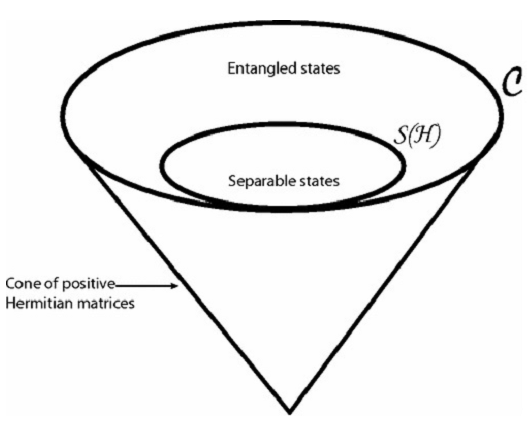
\includegraphics[scale = 0.6]{figs/appendix/QIT sets pictographic img.png}
    \caption{En esta figura se muestra una representación gráfica de las relaciones entre los conjuntos de estados densidad $\mathcal{C}$, el conjunto de estados separables $S(\mathds{H})$ y el conjunto de estados entrelazados $\mathcal{C} \textnormal{ / } \mathcal{S}(\mathds{H})$. Retrieved from \cite{Holik-ECI34}.}
    \label{fig:sets_qit}
\end{figure}

\section{Entrelazamiento y Separabilidad de estados cuántios}

Empezaremos la presente sección con una breve discusión de las condiciones necesarias y suficientes para asegurar la separabilidad de estados cuánticos puros y mixtos en un sistema cuántico bipartito. La distinción entre estados separables y estados entrelazados surge naturalmente del hecho de que no todos los estados en dicho espacio vectorial compuesto ${\bf x} \in A \otimes B$ admiten una descomposición de la forma ${\bf v}_1 \otimes {\bf v}_2$, donde ${\bf v}_1 \in A$ y ${\bf v}_2 \in B$. Surge la necesidad de establecer un criterio para aseverar si cierta matriz densidad pura es entrelazada o no, surgiendo el siguiente resultado. 

Para estados puros, existe un criterio para poder computar si un determinado estado es entrelazado o separable. Enunciamos, entonces, el siguiente teorema de vital importancia a la teoría.

\begin{theo}{Descomposición de Schmidt}{Schmidt decomp}
Dado un estado puro $\ket{\psi} \in \mathbb{H} =\mathbb{H}^{(1)} \otimes \mathbb{H}^{(2)}$ de un sistema cuántico bipartito, existen bases ortonormales $\{\ket{\chi_i^{(1)}}\}_{i=1}^{\dim \mathds{H}_1}$ para $\mathbb{H}^{(1)}$ y $\{ \ket{\chi_i^{(2)}}\}_{i=1}^{\dim \mathds{H}_2}$ para $\mathbb{H}^{(2)}$ tales que 

\begin{equation}
    \ket{\psi} = \sum_{i=1}^{r_\psi} \alpha_{i}  \ket{\chi_i^{(1)}} \otimes \ket{\chi_i^{(2)}},
\end{equation}

donde los coeficientes complejos $\alpha_i$ son los \textit{coeficientes de Schmidt} y siendo $r_\psi \leq \min(\dim \mathds{H}_1, \dim \mathds{H}_2)$ el \textit{número de Schmidt} dado por el teorema de Caratheodory.\footnote{Una demostración del teorema precedente puede encontrarse en \cite{Nielsen.00, B.C.G.STR, HeinzPetruccione}. Notemos que si $\ket{\Psi}$ está normalizado luego $\alpha_i \mbox{\textgreater} 0$ y $\sum_i^{n_s}\alpha_i^2 = 1$.}
\end{theo}

Se dice que un estado $\ket{\Psi} \in \mathbb{H}^{(1)} \otimes \mathbb{H}^{(2)}$ está entrelazado si no puede ser escrito como un producto tensorial $\ket{\phi^{(1)}} \otimes \ket{\phi^{(2)}}$ de estados de los subsistemas. Si $\ket{\Psi}$ puede ser escrito de esta forma, es un \textit{estado producto}.  Un estado será un estado producto \sii su número de Schmidt $n_s \mbox{\textgreater} 1$. Luego podemos enunciar y demostrar el siguiente resultado

\begin{tcolorbox}[colback=red!5!white, colframe=red!50!black, title= Lema sobre \textit{entanglement} de estados puros]

Los estados puros se encuentran entrelazados \textit{sii} sus estados parciales no son puros.
\end{tcolorbox}

\begin{tcolorbox}
Demostración: Sea $\rho = \ket{\psi} \bra{{\psi}}$ un estado puro sobre el sistema global donde  $\ket{\psi}$ un estado genérico sobre $\mathds{H} = \mathds{H}_A \otimes \mathds{H}_B$. Luego su descomposición de Schmidt se escribe como 

$$
\ket{\psi} =\sum _{k=1}^{r_{\psi }}{\sqrt {p_{k}}}(\ket{u_k} \otimes \ket{v_k} ),
$$

donde los $\sqrt {p_{k}}$ son números positivos, $r_{\psi }$ el rango de Schmidt de $\ket{\psi}$ y donde $ \{\ket{u_k} \}_{k=1}^{r_{\psi }}\subset \mathds{H}_{A}$ y $\{\ket{v_k} \}_{k=1}^{r_{\psi }}\subset \mathds{H}_{B}$ son conjuntos ortonormales de estados en los espacios de Hilbert individuales. Luego, el estado está entrelazado \textit{sii} $r_{\psi}$ es mayor estricto a 1. Pero, adicionalmente, el estado parcial se escribirá como

$$
\rho _{A}\equiv \Tr_{B}(\ket{\psi} \bra{\psi})=\sum _{k=1}^{r_{\psi }}p_{k}\,\ket{u_k} \bra{u_{k}} \equiv \ket{\phi}_{A} \bra{\phi}_{A}
$$
\textit{sii} $r_{\psi}=1$. Luego, en tales condiciones,  se sigue que $\rho _{A}$ es pura lo que es equivalente a que $\ket{\psi} = \ket{\psi}_{A}\otimes\ket{\psi}_{B}$ sea separable.
\end{tcolorbox}

La demostración anterior es la base del procedimiento de \textbf{purificación} \cite{Nielsen.00} usada en información cuántica, en la cual es posible construir un estado global puro a partir de un estado mixto introduciendo un sistema de referencia arbitrario. Físicamente esto significa que no es posible asignar un estado puro a los subsistemas si sistema global está descrito por un estado puro. Por tanto, un estado puro $\rho = \ket{\psi}\bra{\psi}$ está entrelazado si la entropía de von Neumann de su estado parcial es no nula. \newline

Por otro lado, existen diferencias cuando el estado $\ket{\psi}$ es un estado mixto. Un estado mixto $\rho \in \mathds{H}_A \otimes \mathds{H}_B$ es separable si existen $\{p_k\}_{k=1}$ tales que

$$
\rho = \sum_{k} p_{k} \rho_{1}^{k} \otimes \rho_{2}^{k} 
$$ 

donde $\{\rho_1^{k}\}_{k=1}$ y $\{\rho_2^{k}\}_{k=1}$ son estados mixtos en sus respectivos subsistemas, sujeto al vínculo de $\sum_{k} p_k = 1$. Caso contrario, $\rho$ es un estado entrelazado. Existen diversos criterios más elaborados para determinar si cierto estado puro o mixto es entrelazado o no, uno de ellos siendo el criterio de separabilidad de Peres \cite{Nielsen.00}. \newline

Habiendo discutido las diferencias entre estados entrelazados y estados separables, podemos construir algunos conjuntos de interés a este trabajo diploma para un sistema cuántico bipartito, a saber:

\begin{itemize}
    \item Los operadores densidad son matrices hermíticas, positivas y de traza unimodular, definiendo estas un conjunto $\mathcal{C} = \{\rho \in GL(n, \mathds{C}) \textnormal{ }| \textnormal{ }\rho^{\dagger} = \rho, \Tr \rho = 1, \rho \geq 0.\}$. Luego $\mathcal{C}$ define un el cono de matrices hermíticas positivas.
    
    \item Adicionalmente, dentro del conjunto anterior, tenemos un conjunto de estados separables $\mathcal{S}(\mathds{H}) \subset \mathcal{C}$ definido como $\mathcal{S}(\mathds{H})=\{ \rho \in \mathcal{C} \textnormal{ | } \exists \{p_k\}_{k=1} \in \mathds{R} \land \exists \{\rho_{k}^{(1, 2)}\}_{k=1} \in \mathds{H}^{1,2} \textnormal{ tal que }\rho = \sum_{k} p_{k} \rho_{k}^{(1)}\otimes\rho_{k}^{(2)}\}$ ie. el conjunto $\mathcal{S}(\mathds{H})$ se define como todos aquellos estados que pueden ser escritos como combinaciones convexas de estados productos. 
    
    \item y un conjunto de estados entrelazados $\mathcal{C} \setminus \mathcal{S}(\mathds{H})$.
\end{itemize}

En la figura \ref{fig:sets_qit} se muestran las relaciones de inclusión de los conjuntos anteriormente definidos. Un problema importante en la formulación matemática de la mecánica cuántica es estudiar la topología del espacio de estados $\mathcal{C}$ para distintas dimensiones del espacio de Hilbert asociado. Esto puede ser estudiado mediante los métodos matemáticos propios a la formulación de topología algebraica.

\section{Estudio formal \textit{ab initio} de las variedades Max-Ent}
\label{hausdorff}

Habiendo definido el conjunto $\mathcal{C}(\mathds{H})$ podemos enunciar el siguiente resultado 

\begin{tcolorbox}[colback=red!5!white, colframe=red!50!black, title= Topología de $\mathcal{C}(\mathds{H})$]

El espacio de estados densidad $\mathcal{C}(\mathds{H})$ es un espacio topológico.
\end{tcolorbox}
\begin{tcolorbox}

La demostración es inmediata. Efectivamente, hay múltiples elecciones de la topología $\mathcal{T}$ que hacen de $(\mathcal{C}(\mathds{H})), \mathcal{T}$ un espacio topológico. Por ejemplo,

\begin{itemize}
    \item La primer opción consiste en construir la \textbf{topología trivial} sobre $\mathcal{C}(\mathds{H})$, esto es $\mathcal{T} = \{\emptyset, \mathcal{C}(\mathds{H})\}$.
    \item Otra opción es, dado que $\mathcal{C}(\mathds{H})$ es un conjunto bien definido, podemos tomar la topología $\mathcal{T}$ como la colección de todos los subconjuntos de $\mathcal{C}(\mathds{H})$ y por tanto se cumplen los axiomas de un espacio topológico. Llamamos a esta elección de $\mathcal{T}$ la \textbf{topología discreta} sobre $\mathcal{C}(\mathds{H})$ \cite{munkres, NakaharaM}.
\end{itemize}
\end{tcolorbox}

Naturalmente, podemos construir otras topologías sobre $\mathcal{C}(\mathds{H})$ que no sean ni la topología trivial ni la discreta. A tal fin, podemos definir el conjunto de operadores sobre este espacio, $\mathds{B}(\mathcal{C}(\mathds{H}))$, como

$$
\mathds{B}(\mathcal{C}(\mathds{H})) = \{ {\bf A} \textnormal{ | } {\bf A}: \mathcal{C}(\mathds{H}) \rightarrow \mathcal{C}(\mathds{H}) \}.
$$

La existencia del producto escalar bien definido \eqref{HS scalar prod} implica que dicho espacio $(\mathds{B}(\mathcal{C}(\mathds{H})),\lgg\cdot, \cdot\rgg_{\textnormal{HS}})$ es un espacio prehilbertiano y la existencia de la norma \eqref{HS norm} implica que este espacio es un espacio normado. Toda norma induce naturalmente una métrica y este espacio puede ser completado de alguna forma, en el sentido de convergencia de series de Cauchy, y podemos considerar a la completación de este espacio, denotada por $(\mathds{B}(\mathcal{C}(\mathds{H}))^{\star},\lgg\cdot, \cdot\rgg_{\textnormal{HS}}^{\star})$, como será un espacio métrico completo y por tanto, un espacio de Banach \cite{HoracioI}. En nuestro caso podemos definir la métrica 

\begin{equation}
    d: \mathds{B}(\mathcal{C}(\mathds{H}))^{\star}\times \mathds{B}(\mathcal{C}(\mathds{H}))^{\star} \rightarrow \mathds{R} \textnormal{ definida como } d({\bf A}, {\bf B})=\lgg {\bf A}, {\bf B} \rgg_{\textnormal{HS}} = \Tr \textbf{A}^{\dagger} {\bf B}
\end{equation}

la cual efectivamente es simétrica, no negativa y cumple la desigualdad triangular. En particular, a la hora de calcular distancias entre estados, podemos definir discos abiertos de radio arbitrario $\epsilon$ sobre dicho espacio, a saber

$$
U_{\epsilon}(\mathcal{C}(\mathds{H})) = \{\sigma \in \mathcal{C}(\mathds{H}) \textnormal{ | } d(\rho, \sigma) \mbox{\textless} \epsilon \}.
$$

Luego, dado que $\mathcal{C}(\mathds{H})$ es un espacio vectorial provisto de una métrica $d$, esta métrica induce naturalmente un \textbf{topología métrica} $\mathcal{T}_d$ sobre dicho espacio y por tanto $(\mathcal{C}(\mathds{H}), \mathcal{T}_d)$ es un espacio métrico. Podemos enunciar el siguiente resultado 

\begin{tcolorbox}[colback=red!5!white, colframe=red!50!black, title= Topología de $\mathcal{C}(\mathds{H})$]

El espacio métrico $(\mathcal{C}(\mathds{H}), \mathcal{T}_d)$ es un espacio de Hausdorff.
\end{tcolorbox}
\begin{tcolorbox}
Como $(\mathcal{C}(\mathds{H}), \mathcal{T}_d)$ es un espacio métrico podemos definir cualesquiera dos puntos $\rho, \sigma \in \mathcal{C}(\mathds{H})$ (físicamente, estados densidad) tales que 

$$
d(\rho, \sigma) = a, a \in \mathds{R}.
$$

Luego, construimos dos discos  abiertos \cite{NakaharaM} de radio $\frac{a}{2}$ entorno a estos dos puntos. Esto es, sean los discos 

\begin{align*}
    U_{\rho} = \{\varsigma \in \mathcal{C}(\mathds{H}) \textnormal{ | } d(\varsigma, \rho) \mbox{\textless} \frac{a}{2}\} \textnormal{ y } 
    V_{\sigma} = \{\varsigma \in \mathcal{C}(\mathds{H}) \textnormal{ | } d(\varsigma, \sigma) \mbox{\textless} \frac{a}{2}\}.
\end{align*}

Luego, si estos no son conjuntos disjuntos $\exists \gamma \in \mathcal{C}(\mathds{H}) \textnormal{ | } \gamma \in U_{\rho} \land \gamma \in V_{\sigma}$. Entonces $d(\gamma,\rho) \mbox{\textless} \frac{a}{2}$ y $d(\gamma,\sigma) \mbox{\textless} \frac{a}{2}$ y por tanto $d(\gamma,\rho) + d(\gamma,\sigma) = a = d(\rho, \sigma)$, resultado que viola la desigualdad triangular de la métrica $d$. Entonces, tal punto $\gamma$ no existe y los entornos $U_{\rho}$ y $V_{\sigma}$ son disjuntos y por tanto, $(\mathcal{C}(\mathds{H}), \mathcal{T}_d)$ es un espacio de Hausdorff. 
\end{tcolorbox}

A continuación, podemos enunciar el siguiente resultado 

\begin{tcolorbox}[colback=red!5!white, colframe=red!50!black, title= Topología de $\mathcal{C}(\mathds{H})$]

El espacio de Hausdorff $(\mathcal{C}(\mathds{H}), \mathcal{T}_d)$ es una variedad topológica.
\end{tcolorbox}
\begin{tcolorbox}
Demostración: La demostración de este lema es engorrosa y excede a este trabajo de diploma. Sin embargo, planteamos las bases de su demotración. Para demostrar que $(\mathcal{C}(\mathds{H}), \mathcal{T})$ es una variedad topologica hemos de demostrar que los entornos a todo punto de dicho espacio son homeomórficos a un subconjunto abierto de $\mathds{R}^{n}$, para algún $n \in \mathds{N}$. Esto es, hemos de demostrar que existen mapeos

$$
\forall \rho \in \mathcal{C}(\mathds{H})\textnormal{, } \exists f_\rho : U_\rho \rightarrow \mathds{R}^{n} 
$$

\begin{itemize}
    \item $f_\rho$ es biyectiva,  
    \item $f_\rho$ es continua y 
    \item la función inversa  $f_\rho^{-1}$ es continua, en el sentido que mapea conjuntos abiertos a conjuntos abiertos. 
\end{itemize}

Luego, precisamente dado que $(\mathcal{C}(\mathds{H}), \mathcal{T}_d)$ es un espacio métrico y usando el teorema de la función inversa \cite{munkres} se sigue que los estos mapeos son homeomórficos y por tanto $(\mathcal{C}(\mathds{H}), \mathcal{T}_d)$ es una variedad topológica.
\end{tcolorbox}

Finalmente, se puede demostrar que $\mathcal{C}(\mathds{H})$ es una variedad diferenciable y una variedad Riemanniana, cuya métrica $g_p: \mathcal{T}_p (\mathcal{C}(\mathds{H})) \rightarrow \mathcal{T}_p (\mathcal{C}(\mathds{H}))$ está relacionada a la divergencia de Kullback-Leibler \cite{Portesi-ECI34, QITGeometry, NakaharaM}. La demostración es altamente no trivial y es tratada en la disciplina de Geometría de la Información Cuántica \cite{Portesi-ECI34, QITGeometry}.

Luego, podemos definir dos conjuntos Max-Ent, subconjuntos al conjunto general $\mathcal{C}(\mathds{H})$, que son relevantes a este trabajo, a saber

\begin{eqnarray*}
\mathcal{S}_{ME,1} = \{ \rho \in \mathcal{C}(\mathds{H}) \textnormal{ | } \exists \{\lambda_k\}_{k=1} \in \mathds{R} \land  \exists \{{\bf O}_{k}\}_{k=1} \in \mathds{B}(\mathcal{C}(\mathds{H}))^{\star}  \textnormal{ tal que }  \rho \propto \exp(-\sum_{i}\lambda_i {\bf O}_i) \}, \\
\mathcal{S}_{ME,2} = \{ \rho \in \mathcal{C}(\mathds{H}) \textnormal{ | } \exists \{\lambda_k\}_{k=1}, \{\gamma_{mn}\}_{m,n=1,_{m \mbox{\textless} n}} \in \mathds{R} 
\land  \exists \{{\bf O}_{k}\}_{k=1} \in \mathds{B}(\mathcal{C}(\mathds{H}))^{\star} \textnormal{ tal que }  \rho \propto \exp(-\sum_{i,j}\lambda_i {\bf O}_i - \gamma_{ij} {\bf O}_i {\bf O}_j ) \}. \end{eqnarray*}

donde los coeficientes $\gamma_{ij}$ son las correlaciones de pares. Estos sub-conjuntos Max-Ent resultan ser además subvariedades a la variedad $\mathcal{C}(\mathds{H})$. La demostración de este resultado excede a este trabajo de diploma y será explayada en futuros trabajos y publicaciones. 
    

\section{Mecánica Cuántica y Elementos de Topología Algebraica}

La mecánica cuántica admite una formulación en términos topología algebraica y dicha abstracción haya su fundamento en que la teoría cuántica posee una invarianza de \textit{gauge} manifiesta $U(1)$ \textit{ie}. no podemos distinguir al estado ${\bf v}$ del estado $e^{i \phi}{\bf v}$, donde $e^{i \phi}$ es una fase multiplicativa global, y por tanto estos estados proveen de la misma información física del sistema cuántico en cuestión. En consecuencia, los estados cuánticos admiten una interpretación como los \textbf{rayos proyectivos} en un \textbf{espacio de Hilbert proyectivo} $P(\mathds{H})$ de un espacio de Hilbert $\mathds{H}$ \cite{Hatcher:AT, GoldbartStone}. En dicho espacio, no distinguimos entre los estados ${\bf v}$ y $\lambda {\bf v}$ con $\lambda$ no nulo.

Definimos un \textbf{rayo} como el conjunto de todos los vectores en el subespacio uno-dimensional generado por un estado ${\psi}$ sobre el cuerpo $F = \mathds{C}$. El rayo asociado es 

$$
R_{\psi} = \{{\phi} \in \mathds{H}\textnormal{ | } \exists \lambda \in \mathds{C}_{0} \textnormal{ tal que } {\phi} = \lambda {\psi}\}.
$$

Todos los vectores de este conjunto son físicamente indistinguibles y, frente a una medida, devolverán los mismos resultados. Luego, es posible construir una relación de equivalencia sobre dicho espacio de Hilbert $\sim$, a saber:

$$
 \phi \sim \psi \Longleftrightarrow \phi \in R_{\psi},
$$

la cual efectivamente es efectivamente reflexiva, simétrica y transitiva \cite{munkres, GoldbartStone}. Finalmente, el espacio de Hilbert proyectivo $P(\mathds{H})$ se construye como el conjunto cociente entre el espacio de Hilbert $\mathds{H}$ y la relación de equivalencia $\sim$:

$$
P(\mathds{H}) = (\mathds{H}-\{0\})/\sim.
$$
 
En otras palabras, el espacio de Hilbert proyectivo $P(\mathds{H})$ consiste en el conjunto de todas las clases de equivalencia $[{\bf v}, {\bf w}]$ de vectores no nulos ${\bf v}, {\bf w} \in \mathds{H}$ que son proporcionales entre sí. En particular, si $\mathds{H}$ es finito dimensional, resulta que el espacio de Hilbert proyectivo es isomorfo al \textbf{espacio complejo proyectivo}, a saber:

\begin{equation}
    P(\mathds{H}) = \mathds{C}P^{n-1},
\end{equation}

siendo $n=\dim\mathds{H}$. Adicionalmente, el conjunto de estados producto es un subconjunto del espacio complejo proyectivo $\mathds{C}P^{nm-1}$. Dicho subconjunto está definido por un número finito de ecuaciones polinómicas homogéneas que forman una \textit{variedad algebraíca}, la \textbf{variedad de Segre} \cite{Hatcher:AT}. 

El espacio complejo proyectivo más simple es $\mathds{C}P^{1}$, la línea compleja proyectiva, resulta ser isomorfa a la 2-esfera real $\mathcal{S}^{2}$, $\mathds{C}P^{1} \simeq \mathcal{S}^{2}$. Efectivamente,
mediante el mapeo estereográfico, la clase de equivalencia $[\zeta_{1}, \zeta_{2}] \in \mathds{C}P^{1}$ puede ser puesta en correspondencia a un único punto ${\bf n} \in \mathcal{S}^{2}$. La interpretación física inmediata implica que todo 3-vector ${\bf n}$ puede ser obtenido mediante un valor de expectación de las matrices de Pauli en un estado espinorial, por tanto un espinor normalizado puede ser pensado como un punto en $\mathcal{S}^{3}$. Esta correspondencia uno a uno entre $[\zeta_1, \zeta_2] \leftrightarrow {\bf n}$ da origen al llamado \textbf{mapeo de Hopf} \cite{GoldbartStone}, a saber:
$$
\mathfrak{Hopf}: \mathcal{S}^{3} \rightarrow \mathcal{S}^{2},
$$

el cual es un mapeo difeomórfico. Adicionalmente, estudiando los fibrados tangentes,
es posible construir mapeos topológicamente no triviales que relacionan las 1,2 y 3-esferas:

$$
\mathcal{S}^{1} \rightarrow \mathcal{S}^{3} \xrightarrow{{\mathfrak{hopf}}} \mathcal{S}^{2},
$$

es decir que el espacio $\mathcal{S}^{1}$ es un \textit{embedding} en la 3-esfera $\mathcal{S}^{3}$, la cual a su vez puede ser proyectada en la 2-esfera $\mathcal{S}^{2}$. Esta fibración es altamente no trivial, pues los espacios son globalmente topológicamente diferentes y no pueden ser escritos como productos cartesianos entre sí. 

Estos resultados topológicos inducen una representación natural para el espacio de estados de los 1-qubits, la topología del espacio $\mathcal{C}$ definido anteriormente es la conocida esfera de Bloch. Podemos establecer los siguientes isomorfismos:

$$
\mathcal{C} \approx P(\mathds{H}_{2}) \approx \mathds{C}P^{1} \approx \mathcal{S}^{2} \rightarrow \mathds{C}_{\infty},
$$

siendo $\mathds{C}_{\infty}$ la esfera de Riemann. Otra forma de entender estos resultados consiste en notar que las simetrías de un sistema cuántico con un espacio de Hilbert $\mathds{H}$ están dadas por la representación de un grupo de simetría 

$$
G \rightarrow PU(\mathds{H})
$$

en el grupo unitario proyectivo del esapcio de Hilbert. Dicho grupo actúa naturalmente sobre el espacio proyectivo $P(\mathds{H})$ y no sobre $\mathds{H}$. Consideremos ahora una partícula no relativista de espín $\frac{1}{2}$: esta tiene una simetría rotacional con representación

$$
SO(3) \rightarrow PU(\mathds{H}).
$$

Pero dichas representaciones proyectivas tienen una correspondencia uno a uno con las representaciones del grupo cubrimiento de $SO(3)$, el grupo $SU(2)$

$$ 
SU(2) \rightarrow U(\mathds{H}). 
$$

Como el grupo $SU(2)$ es un grupo compacto, cuya variedad es la 3-esfera $S^3$ \cite{HoracioI}, sus representaciones unitarias son finito dimensional, y por tanto luego tenemos que 

$$
P(\mathds{C}^2) \approx CP^{1}.
$$

\chapter{Aproximaci\'on perturbativa a la din\'amica de Lindblad}
\label{ApendixA}
En este apéndice estudiaremos algunas cuestiones relacionadas a la dinámicas del sistema de dos bosones, como así también propiedades de sistemas bosónicos generales. 

\section{Din\'amica Abierta de un sistema de dos bosones}

En esta sección, usaremos el Hamiltoniano \eqref{model3.1_hamiltonian} para estudiar una dinámica abierta mediante una ecuación de Lindblad, con unos operadores de colapso \textit{a priori} desconocidos. Dichos operadores de colapso serán elegidos de forma de asegurar la termalización del sistema independientemente del estado inicial estudiado. 

Notamos que las ecuaciones de evolución, tanto para un sistema abierto como un sistema cerrado, son ecuaciones diferenciales de primer orden en la variable temporal Lifshitz-continuas. Por otro lado, no sabiendo cuales son los operadores de colapso adecuados, empezaremos nuestro estudio mediante el uso del teorema de Picard \cite{CohenTannoudji1989} para escribir la solución $\rho_{AB}(t)$ a la ecuación de Lindblad \eqref{Lindblad eq.} a tiempos cortos. En tal caso, es justificado el uso del teorema de Picard para escribir una solución aproximada, a saber

\begin{equation}
    \rho_{AB}(t) \approx \rho_{AB}(t_0)-i\int_{0}^{t} dt' [\mathbf{H}_{I}(t'), \rho_{AB}(t')] - \int_{0}^{t} dt' \int_{0}^{t'} dt'' [\mathbf{H}_{I}(t''),[\mathbf{H}_{I}(t'), \rho_{AB}(t')]] + \ldots,
    \label{model3.1_rho_initial}
\end{equation}

donde $\mathbf{H}_I = \alpha({\mathbf a}^{\dagger}{\mathbf b}+ {\mathbf b}^{\dagger}{\mathbf a})$ es el Hamiltoniano de interacción. 

A continuación, deseamos enfocarnos únicamente en { la evolución de uno de los modos}. A tal fin, hemos de {\color{red} } eliminar las correlaciones con la cavidad tomando la traza parcial sobre dicho subsistema del estado escrito en \eqref{model3.1_rho_initial}.

La traza parcial sobre el subsistema $B$ de los términos $\mathcal{O}(\alpha)$ se anulan (la traza de un valor de expectación se anula), por lo que el término de orden dominante es a $\mathcal{O}(\alpha^2)$. Para hacer dicho cálculo, hacemos uso del principio Max-Ent, tomando un estado producto de estados gaussianos, $\rho_{AB} = \rho_{A} \otimes \rho_B$ donde tanto $\rho_A$ como $\rho_B$ son estados gaussianos. En particular, tomaremos

\begin{equation}
\rho_{B} = \frac{1}{\mathcal{Z}} e^{-\zeta b^{\dagger}b }
\label{model1_rhoB}
\end{equation}

donde $\mathcal{Z}$ es la función de partición asociada al sistema $B$ y siendo $\zeta$ una constante \textit{a priori} desconocida. Para tener el contacto con la termodinámica, necesitamos conocer dicha función de partición. Acorde a la mecánica estadística, dado un observable físico $\mathbf{O}$ su valor de expectación en el ensamble es 

\begin{equation}
    \lgg \mathbf{O} \rgg = \frac{1}{\mathcal{Z}}\Tr \bigg(\mathbf{O}e^{-\zeta b^{\dagger}b }\bigg).
\end{equation}

En particular, esto es válido para el operador número del subsistema $B$: $\mathbf{n}_B = {\mathbf b}^{\dagger}{\mathbf b}$. Entonces,

\begin{equation}
    n_B = \Tr\bigg({\mathbf b}^{\dagger}{\mathbf b}e^{-\zeta {\mathbf b}^{\dagger}{\mathbf b} }\bigg) = \frac{1}{\mathcal{Z}} \sum_{n} n e^{-\zeta n} ,
\end{equation}

luego

\begin{equation}
    \zeta = \log \left(1 + \frac{1}{n_B}\right).
\end{equation}

Conociendo esta información, tendremos que $\Tr_{B} \bigg[{\bf H}_{I},[{\bf H}_{I},\rho_{AB}]\bigg]$ podrá ser reescrita como

\begin{equation}
\Tr_{B} \bigg[{\bf H}_{I},[{\bf H}_{I},\rho_{AB}]\bigg] = \gamma_1 {\mathbf a}\rho_{A} {\mathbf a}^{\dagger} + \gamma_2 {\mathbf a}^{\dagger} \rho_{A}{\mathbf a} - \frac{\gamma_1 + \gamma_2}{2} \{{\mathbf a}^{\dagger}{\mathbf a},\rho_{A}\} - \gamma_2 \rho_{A},  
\label{model3.1_Lindblad}
\end{equation}

donde $\gamma_1 = -2\alpha^2n_B^2\left(1+\frac{1}{n_B}\right)^2\left(1-\frac{n_B}{n_B+1}\right)$ y $\gamma_2 = -2\alpha^2n_B^2\left(1+\frac{1}{n_B}\right)\left(1-\frac{n_B}{n_B+1}\right)$. Comparando \eqref{model3.1_Lindblad} con \eqref{Lindblad eq.}, observamos que \eqref{model3.1_Lindblad} efectivamente se corresponde a una ecuación de Lindblad con factores de colapso dados por $\gamma_1$ y $\gamma_2$ con operadores de colapso dados por ${\bf C}_1 = {\mathbf a}$ y ${\bf C}_2 = {\mathbf a}^{\dagger}$. La ecuación \eqref{model3.1_Lindblad} ha eliminado toda la información del sistema $B$ dejando solamente las "consecuencias" de dichas correlaciones entre los subsistemas.

%Cabe destacar, que efectivamente $\gamma_2 \mbox{\textgreater} \gamma_1$. 

Surge otra interrogante, ¿qué sucede si evolucionamos un estado gaussiano? Es decir, nos interesa estudiar la dinámica de Lindblad del estado gaussiano $\rho_{A} = \frac{1}{\mathcal{Z}} e^{-\zeta {\mathbf a}^{\dagger} {\mathbf a}}$ con $\mathcal{Z} = \frac{1}{1-e^{-\Gamma}}$ y $\Gamma= \log\left(1+\frac{1}{n}\right)$. Dicha dinámica, será evidentemente, gaussiana. Entonces tendremos

\begin{align}
    \frac{d}{dt} \lgg {\mathbf a}^{\dagger}{\mathbf a} \rgg = \Tr \left({\mathbf a}^{\dagger}{\mathbf a}\frac{d\rho}{dt}\right)
    = \Tr \bigg[\gamma_1 {\mathbf a}^{\dagger}{\mathbf a}^{\dagger}{\mathbf a}\rho+ \gamma_2{\mathbf a}^{\dagger}{\mathbf a}^{\dagger}{\mathbf a}\rho - \gamma_1 ({\mathbf a}^{\dagger}{\mathbf a})^2 \rho - \gamma_2 ({\mathbf a}^{\dagger}{\mathbf a}({\mathbf a}^{\dagger}{\mathbf a}+1))\rho\bigg].
\end{align}

Calculando los términos anteriores obtendremos una ecuación diferencial. Renombrando $\lgg {\mathbf a}^{\dagger}{\bf a} \rgg = n$ tendremos 

\begin{Omitir}
\begin{equation}
    \frac{dn}{dt}= 4\gamma_1 n^2 + 2\gamma_2 n(2n+1) - 2\gamma_1 n(2n+1)-\frac{\gamma_2n}{(n+1)^2}
\end{equation}
\end{Omitir}

\begin{equation}
    \frac{dn}{dt}= 4\gamma_2 n^2 + 2(\gamma_2 - \gamma_1) n - \frac{\gamma_2 n}{(n+1)^2}
    \label{eq:dif_model1}
\end{equation}

La ecuación precedente es una ecuación diferencial a primer orden no lineal, Lifshitz continua para $n \in \mathds{R}_{+}$. No se dispone de una solución exacta a la misma por lo que recurrimos a una solución numérica para estudiar el comportamiento de la misma. Se utiliza el paquete \textbf{odeint} del lenguaje Python para obtener un \textit{plot} de $n$ $vs$. $t$, mostrado a continuación

\begin{figure}
    \centering
    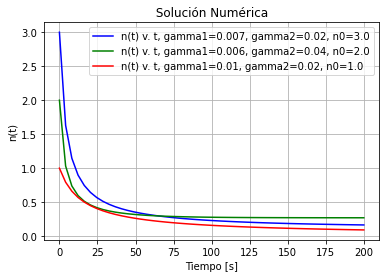
\includegraphics[scale=0.75]{figs/tdd_modelito1_sol_eq_diff_modificada.png}
    \caption{Se muestra un \textit{plot} de la solución numérica de la \eqref{eq:dif_model1} obtenida mediante la función odeint del paquete scipy del lenguaje Python para distintos parámetros de $\gamma_1,\gamma_2$ y $n_0$. Notamos que las soluciones tienen asíntotas horizontales cerca de cero pero distintas a cero.}
    \label{fig:tdd_modelito1_sol_eq_diff_odeint_multiples}
\end{figure}

En la figura \ref{fig:tdd_modelito1_sol_eq_diff_odeint_multiples} se muestran distintos plots de $n$ $vs$. $t$ para distintas condiciones iniciales de $\gamma_1, \gamma_2$ y número inicial de partículas $n_0$. Como se puede apreciar, vemos que el sistema termaliza, volviendo a su estado de equilibrio.

Concluímos que la dinámica de Lindblad para el Hamiltoniano \eqref{model3.1_hamiltonian} con operadores de colapso bosónicos resultará en una termalización a un estado con un número de ocupación fijo, resultado completamente independiente de la identidad del estado inicial del sistema.

\section{Din\'amica de Lindblad de un sistema bos\'onico}

En este capítulo nos interesará estudiar una dinámica abierta de un sistema bosónico con la ecuación de Lindblad. En particular, tomaremos un Hamiltoniano bosónico simple ${\bf H} = \Omega {\bf a}^{\dagger} {\bf a},$ con operadores de colapso dados por $\mathbf{C}_1 = {\bf a}$ y $\mathbf{C}_2 = {\bf a}^{\dagger}$ y factores de colapso $\gamma_1$ y $\gamma_2$ genéricos. Ántes de comenzar nuestros cálculos analíticos, ya podremos concluir en base a los resultados obtenidos en la sección anterior que el estado inevitablemente termalizará. Procederemos, a continuación, a realizar los cálculos analíticos y constatar si dichos resultados se condicen con los obtenidos anteriormente. 

Escribimos la ecuación de Lindblad

\begin{equation}
   \dot{\rho} = {\bf i}[\mathbf{H}_2,\rho] + \gamma_1 {\bf a}\rho {\bf a}^{\dagger} + \gamma_2 {\bf a}^{\dagger} \rho{\bf a} - \frac{\gamma_1 + \gamma_2}{2} \{{\bf a}^{\dagger}{\bf a},\rho\} - \gamma_2 \rho.  
   \label{model3.2_Lindblad}
\end{equation}

Esta ecuación podrá ser reescrita como

$$
\frac{d\rho}{dt} = \mathbf{K}(\rho),
$$

donde $\mathbf{K}$ es una funcional lineal. Podremos entonces tomar una solución perturbativa, $\rho(t) = \alpha_0 \rho_0 + \alpha_1\rho1 + \ldots$ donde $\alpha_0, \alpha_1, \ldots$ son coeficientes reales y los $\rho_0, \rho_1, \ldots$ son los autovectores del operador diferencial anterior, que cumplirán que $\mathbf{K}(\rho) = 0$, $\mathbf{K}(\rho_1) = - \lambda_1 \rho_1$ etc. El estado evolucionado tendrá la forma 

$$
\rho (t) = \rho_0 + e^{-\lambda_1t} \rho_1 + \ldots 
$$

luego el comportamiento de esta solución a largos plazos, por ejemplo si el estado termaliza o no, dependerá de las características de dichos autovalores $\lambda_{\mu}$. 


Nos interesa hallar las soluciones a dichas ecuaciones usando este método perturbativo. Sabemos que los autoestados del Hamiltoniano bosónico son los estados de Fock, $\ket{n}$. En consecuencia, podremos construir las soluciones de dos formas

\begin{itemize}
    \item Primero, una de las posibles soluciones al sistema \eqref{model3.2_Lindblad} es que dicha solución sea proporcional a $\sum_{n} \ket{n}\bra{n}$, donde la suma se realiza sobre todos los estados accesibles al sistema. Sin pérdida de generalidad, tomaremos un estado solución como 
    
    \begin{equation}
        \rho=\sum_{n} \sum_{\mu} e^{-\lambda_{\mu}t} \mathcal{Q}_{n}^{\mu} \ket{n}\bra{n},
    \label{model3.2_diagonal}
    \end{equation}
    
    
    \item Otra posible solución es que dicho estado sea proporcional a $\sum_{n, m\neq n} \ket{n} \bra{m}$
    a realizarse sobre todos los estados accesibles del sistema. Entonces, una posible solución será
    
    \begin{equation}
        \rho= \sum_{n,m} \sum_{\nu} e^{-\lambda_{\mu} t} \mathcal{P}_{n}^{\mu} \ket{n}\bra{m} \label{model3.2_no_diagonal}
    \end{equation}
    
     donde $\lambda_{\mu}$ y $\mathcal{P}_{n}^{\mu}$ son factores reales a determinar.
\end{itemize}

Empezaremos introduciendo \eqref{model3.2_diagonal} en \eqref{model3.2_Lindblad}, tomando el overlap a izquierda con $\bra{m}$ y a derecha con $\ket{m}$ y denotando a $\bra{m}\rho\ket{m} = \rho_{m}$ tendremos 

\begin{equation}
    \dot{\rho}_n = \Gamma_1 (n+1) \rho_{n+1} + \Gamma_2 n \rho_{n-1} - (\Gamma_1 + \Gamma_2)n \rho_n - \Gamma_2 \rho_n.
    \label{model3.2_lindblad_diagonal}
\end{equation}

Esta ecuación diferencial es, en realidad, un sistema de infinitas ecuaciones diferenciales lineales a coeficientes constantes acopladas la cual podrá ser resuelta mediante la diagonalización de la matriz de coeficientes. Formalmente, \eqref{model3.2_lindblad_diagonal} podrá ser escrita como

\begin{equation*}
    \frac{d\rho}{dt} = \Omega \rho,
\end{equation*}

donde ${\Omega} $ es la matriz de coeficientes que relaciona a los distintos $\rho_{n}$. Para facilitar dicha diagonalización, conviene realizar un cambio de base de forma que dicha matriz sea simétrica. El nuevo estado será $\tilde{\rho} = \mathcal{S}^{-1} \rho$ donde los elementos de la matriz de cambio de base es

$$S_{nm} = \left(\frac{\Gamma_2}{\Gamma_1}\right)^{n} \delta_{nm}$$.

Introduciendo este cambio de base en \eqref{model3.2_lindblad_diagonal} tendremos que 


\begin{equation}
    \left(-\frac{\lambda_\mu}{\sqrt{\Gamma_1 \Gamma_2}} + \left(1+\frac{\Gamma_2}{\Gamma_1}\right)\sqrt{\frac{\Gamma_1}{\Gamma_2}} n + \sqrt{\frac{\Gamma_2}{\Gamma_1}}\right) \tilde{\rho}_n - (n+1)\tilde{\rho}_{n+1} - n\tilde{\rho}_{n-1} = 0,
\end{equation}

Este sistema de ecuaciones se traduce en el siguiente sistema matricial

\begin{equation}
    \left(\begin{array}{cccc}
       -{\lambda_\mu}+ \left(1+\frac{\Gamma_2}{\Gamma_1}\right)\Gamma_1 + \Gamma_2 & -2\sqrt{\Gamma_1 \Gamma_2} & 0 & \cdots \\
     -2\sqrt{\Gamma_1 \Gamma_2} & -{\lambda_\mu} + 2\left(1+\frac{\Gamma_2}{\Gamma_1}\right)\Gamma_1 + \Gamma_2 & -3\sqrt{\Gamma_1 \Gamma_2} &  \cdots \\ 
     0 & -3\sqrt{\Gamma_1 \Gamma_2} & \ddots & \ddots \\
        \vdots & \cdots & \ddots \\
    \end{array}\right) \left(\begin{array}{lc}
        {\tilde{\rho}}_{1}  \\
        {\tilde{\rho}}_{2}  \\
        \vdots   \\
        {\tilde{\rho}}_{n}  \\  
        \vdots
    \end{array} \right) = \mathbf{0}
    \label{model3.2_matrix_system}
\end{equation}

De la ecuación anterior encontramos que los coeficientes $\lambda_\mu$ son los autovalores del sistema. Obtener la forma analítica de dichos autovalores no es inmediato puesto que lidiamos con un sistema de infinitas ecuaciones lineales acopladas, sin embargo podemos obtener algunos resultados cualitativos. Numéricamente, mediante el paquete \textbf{scipy.linalg} del lenguaje Python es posible implementar un procedimiento de \textit{cut-off} de la matriz a una dimensión finita y obtener una aproximación de los autovalores. Específicamente, es relevante si el sistema \eqref{model3.2_matrix_system} admite al autovalor nulo. Mediante un cálculo analítico del sistema de ecuaciones observamos que, efectivamente, admite al autovalor nulo. Por otro lado, numéricamente, observamos que los autovalores tienen una cota inferior la cual tiende a cero a medida que aumenta el \textit{cut-off} utilizado. Adicionalmente, todos los autovalores son estrictamente positivos. 

Habiendo finalizado el estudio con los estados \eqref{model3.2_diagonal}, pasamos a estudiar la dinámica de Lindblad usando los estados no diagonales \eqref{model3.2_no_diagonal}. Repitiendo los mismos procedimientos que hicimos anteriormente para las componentes diagonales, tendremos la siguiente ecuación 

\begin{equation}
    \left(-\lambda_{\mu}- \frac{\Gamma_1+\Gamma_2}{2}(m+m') - \Gamma_2\right)\rho_{mm'} + \Gamma_1\sqrt{(m+1)(m'+1)}\rho_{m+1,m'+1} + \Gamma_2 \sqrt{mm'}\rho_{m-1,m'-1} = 0,
    \label{model3.2_lindblad_2}
\end{equation}

donde $\bra{m}\rho\ket{m'} = \rho_{mm'}$. Nuevamente, disponemos la forma analítica de los autovalores $\lambda_\mu$ pero podremos inferir algunas propiedades a partir de \eqref{model3.2_lindblad_2}. A diferencia de las componentes diagonales, el sistema \eqref{model3.2_lindblad_2} no admite al valor nulo como autovalor. Sin embargo, el conjunto de autovalores $\{\lambda_i, i = 0,1,\ldots\}$ son siempre positivos.

Entonces concluimos que a tiempos largos el sistema inevitablemente termalizará, independientemente de si el estado sea diagonal o no en la base de autoestados del operador número bosónico. 

\section{Din\'amica de Lindblad y traslaciones}

Probaremos un resultado importante de las ecuaciones de Linblad. Buscamos estudiar la eventualidad de la termalización de un estado traslado si el estado no traslado se termaliza.

Tomemos un Hamiltoniano bosónico con un acoplamiento espín-bosón, a saber

\begin{equation}
    {\bf H} = \Omega {\bf a}^{\dagger}{\bf a} + {\bf S}_z + {\bf S}_z (\zeta {\bf a}^{\dagger} + \zeta^* {\bf a}), 
    \label{model3.3_hamiltonian}
\end{equation}

donde $\zeta$ es un número complejo. 

Nos interesa estudiar la evolución temporal abierta de un estado mediante la ecuación de Lindblad \eqref{Lindblad eq.} haciendo uso de los operadores de colapso ${\bf a}, {\bf a}^{\dagger}$. A tal fin, consideramos un estado gaussiano inicial $\rho = e^{- \Omega {\bf a}^{\dagger} {\bf a}}$, sobre el cual le aplicaremos una traslación a saber

\begin{equation}
    \tilde{\rho} (\varsigma) =  T(\varsigma) e^{-\zeta {\bf a}^{\dagger}{\bf a}} T(\varsigma)^{\dagger} = \exp\bigg(-\Omega {\bf a}^{\dagger}{\bf a} +\varsigma^{*} {\bf a} +\varsigma {\bf a}^{\dagger} + \varsigma^{*}\varsigma\bigg),
    \label{model 1 translated rho}
\end{equation}

donde $T(\varsigma) = e^{\varsigma^{*}{\bf a}-\varsigma {\bf a}^{\dagger}}$ es el operador (unitario) de traslación para $\varsigma \in \mathds{C}$ \cite{CohenTannoudji1989}. Este estado es un estado Max-Ent que incluye hasta correlaciones de pares. 
Entonces, introduciendo este estado en la ecuación de Lindblad \eqref{Lindblad eq.} para algunos coeficientes de colapso $\gamma_1, \gamma_2$ genéricos tendremos 

\begin{equation}
    \dot{\tilde{\rho}}(\varsigma) = i [\tilde{\mathbf{H}}(\varsigma), \tilde{\rho}(\varsigma)] + \gamma_1 \tilde{{\bf a}}(\varsigma) \tilde{\rho}(\varsigma) \tilde{{\bf a}}^{\dagger}(\varsigma) + \gamma_2 \tilde{{\bf a}}^{\dagger}(\varsigma)\tilde{\rho}(\varsigma) \tilde{{\bf a}}(\varsigma) - \frac{1}{2} \{{\gamma_1\tilde{{\bf a}}^{\dagger}}(\varsigma)\tilde{{\bf a}}(\varsigma) + \gamma_2 \tilde{{\bf a}}(\varsigma)\tilde{{\bf a}}^{\dagger}(\varsigma) ,\tilde{\rho}(\varsigma)\} 
    \label{lindblad model1}
\end{equation}

donde $\tilde{\mathbf{H}} = T(\varsigma) \mathbf{H} T(\varsigma)^{\dagger} $ y donde se ha usando que 

\begin{align}
\tilde{{\bf a}}(\varsigma) = T(\varsigma) {\bf a} T(\varsigma)^{\dagger} = {\bf a} + \varsigma,
\\
\tilde{{\bf a}}^{\dagger}(\varsigma) = T(\varsigma) {\bf a}^{\dagger} T(\varsigma)^{\dagger} = {\bf a}^{\dagger} + \varsigma.
\label{model 1 trl2}
\end{align}

Formalmente, \eqref{lindblad model1} es una ecuación de Lindblad. Continuando los desarrollos tendremos

\begin{equation}
\frac{d\tilde{\rho}}{dt}={\bf i }[\zeta {\bf a}^\dagger {\bf a} +\varsigma {\bf a}^\dagger -\varsigma^* {\bf a} ,\tilde{\rho}]+
\gamma_1 {\bf a}\tilde{\rho} {\bf a}^\dagger +
\gamma_2 {\bf a}\tilde{\rho} {\bf a}^\dagger-\frac{\{\gamma_1 {\bf a}^\dagger{\bf a}+\gamma_2 {\bf a}{\bf a}^\dagger,\tilde{\tilde{\rho}}\}}{2}.
\end{equation}

En particular, para una traslación infinitesimal tendremos $\tilde{\rho}(\varsigma) = T(\varsigma) \rho T(\varsigma)^{\dagger}$ con $T(\varsigma)= \exp(\delta\varsigma^{*} {\bf a} - \delta\varsigma {\bf a}^{\dagger})$ de manera que 

\begin{equation}
    T(\varsigma) {\bf a} T(\varsigma)^{\dagger} = {\bf a} - \delta\varsigma.
\end{equation}

Sustituyendo esto en \eqref{lindblad model1}, usando las relaciones en \eqref{model 1 trl2} y agrupando los términos tendremos

\begin{Omitir}
\begin{align}
\frac{d \tilde{\rho}}{dt}={\bf i }[\zeta  T(\varsigma)^\dagger {\bf a}^\dagger {\bf a} T(\varsigma) +\varsigma  T(\varsigma)^\dagger{\bf a}^\dagger  T(\varsigma) -\varsigma^*  T(\varsigma)^\dagger {\bf a}T ,\tilde{\rho}] \\
+  T(\varsigma)^\dagger \gamma_1 {\bf a} T(\varsigma) \tilde{\rho}  T(\varsigma)^\dagger {\bf a}^\dagger   T(\varsigma)+
 T(\varsigma)^{\dagger}\gamma_2 {\bf a} T(\varsigma) \tilde{\rho} T(\varsigma)^\dagger {\bf a}^\dagger  T(\varsigma) \\
-\frac{\{\gamma_1  T(\varsigma)^\dagger{\bf a}^\dagger{\bf a}  T(\varsigma)+\gamma_2  T(\varsigma)^\dagger{\bf a}{\bf a}^\dagger  T(\varsigma), \tilde{\rho}\}}{2}
\end{align}
\end{Omitir}

\begin{dmath}
\frac{d \tilde{\rho}}{dt}={\bf i } \bigg[\zeta {\bf a}^\dagger {\bf a},\tilde{\rho}\bigg]+ \
\gamma_1 {\bf a} \tilde{\rho} {\bf a}^\dagger+
\gamma_2 {\bf a}^\dagger\tilde{\rho} {\bf a}
-\frac{\{\gamma_1 {\bf a}^\dagger{\bf a} +\gamma_2 {\bf a}{\bf a}^\dagger, \tilde{\rho}\}}{2} \\
+{\bf i }\bigg[(\varsigma^* - \zeta \delta \varsigma^* -\frac{(\gamma_2-\gamma_1) \delta \varsigma^* 
}{2{\bf i}}) {\bf a} + 
         (\varsigma - \zeta \delta \varsigma +\frac{ (\gamma_1-\gamma_2)\delta \varsigma}{2{\bf i}}){\bf a}^\dagger,\tilde{\rho}\bigg].
\end{dmath}

Finalmente, eligiendo $\delta \varsigma=\frac{\zeta}{(\zeta \delta \varsigma -\frac{ (\gamma_1-\gamma_2)}{2{\bf i}}) }$ de manera que

\begin{equation}
    \zeta - \zeta \delta \varsigma +\frac{ (\gamma_1-\gamma_2)\delta \varsigma}{2{\bf i}}=0
\end{equation}

\begin{align}
\frac{d \tilde{\rho}}{dt}={\bf i }[\zeta {\bf a}^\dagger {\bf a},\tilde{\rho}]+ \gamma_1 {\bf a} \tilde{\rho} {\bf a}^\dagger+
\gamma_2 {\bf a}^\dagger\tilde{\rho} {\bf a}
-\frac{\{\gamma_1 {\bf a}^\dagger{\bf a} +\gamma_2 {\bf a}{\bf a}^\dagger, \tilde{\rho}\}}{2}    
\end{align}

que es la ecuación de Lindblad \eqref{Lindblad eq.} para un oscilador, centrado en el origen, que relaja exponencialmente a un estado de equilibrio térmico. De esta manera, $\rho$ relajará a un estado de equilibrio térmico, trasladado en $\delta \varsigma$. Con esto también se demuestra que la estructura algebraica de las traslaciones (unitarias), que resulta ser un grupo continuo, forman una simetría de la ecuación de Lindblad.  

\chapter{El c\'odigo}
\label{AppendixB}

En el presente apéndice, explicaremos los algoritmos implementados para la realización de los cálculos numéricos del presente trabajo de diploma. 

\section{Base del algoritmo de la aproximaci\'on Max-Ent}

En esta sección explicaremos el algoritmo utilizado para el cálculo de las entropías relativas y valores de expectación de operadores del capítulo \ref{chapter5}. Explicaremos el código numérico usado para el caso particular de estudiar el modelo de dos sistemas bosónicos acoplados y su aproximación Max-Ent.

Como primera medida, declaramos los paquetes a utilizar. Usaremos \textbf{QuTip} para las simulaciones de los sistemas cuánticos, \textbf{matplotlib.pyplot} el cual se encargará de las salidas gráficas, \textbf{Numpy} para los diversos cálculos científicos a realizar, \textbf{scipy.optimize} será usado para hallar el estado max-ent y minimizar el funcional escrito en el \textit{right-hand side} de \eqref{max-ent_def1}, el paquete \textbf{pickle} implementa protocolos binarios para serializar y deserializar una estructura de objetos, el paquete \textbf{cmath} es usado para hacer cálculos con números complejos y finalmente el paquete \textbf{datetime} para manipular tiempos y horas.

\begin{lstlisting}[language=Python]
import QuTip 
import matplotlib.pyplot as plt 
import numpy as np 
import scipy.optimize as opt 
import pickle 
import cmath 
import datetime 
\end{lstlisting}

En primera instancia, procedemos a escribir las rutinas numéricas de los métodos matemáticos a usar. Primero, hemos de definir una lista de operadores que actúen sobre el espacio de Hilbert global en términos de los operadores que actúan sobre cada subsistema. 

\begin{lstlisting}[language=Python]
def prod_basis(b1, b2):
    return [qutip.tensor(b,s) for b in b1 for s in b2]


def scalar_prod(op1,op2,rho0=None):
    if op1.dims[0][0]!=op1.dims[0][0]:
        return None
    if rho0 is None:
        rho0 = qutip.qeye(op1.dims[0])/op1.dims[0][0]
    return ((op1.dag()*op2+op2.dag()*op1)*rho0).tr()
\end{lstlisting}

A continuación definimos la rutina numérica que evalúa el producto interno de Hilbert-Schmidt ponderado \eqref{HS scalar prod pond}. Definimos aquí la rutina numérica para el proceso de ortonormalización de Gram-Schmidt

\begin{lstlisting}[language=Python]
def base_orto(ops,rho0):
    dim = ops[0].dims[0][0]
    base = []
    # hacer gramm schmidt
    for op in ops:
        coeff = [scalar_prod(op2,op, rho0) for op2 in base]
        op_mod = op - sum([ c*op2 for c, op2 in zip(coeff, base)])
        op_mod = op_mod/np.sqrt(scalar_prod(op_mod,op_mod, rho0))
        base.append(op_mod)
    return base
\end{lstlisting}

Mediante la función definida a continuación, tomaremos por referencia a un operador genérico $\mathbf{K}$ y se lo proyecta en una base de operadores ortonormalizada reproduciendo una descomposición de Fourier-Bessel 

\begin{lstlisting}[language=Python]
def proj_op(K,base,rho0):
    return sum([   scalar_prod(b, K,rho0) * b for b in base])
\end{lstlisting}

A continuación, implementamos las rutinas numéricas que permiten calcular el logaritmo y la raíz cuadrada de una matriz en términos de sus autovalores y autovectores. 

\begin{lstlisting}[language=Python]

def logM(rho):
    vals, vecs = rho.eigenstates()
    return sum([np.log(val)*vec*vec.dag() for val,vec in zip(vals, vecs) if val>0])

def sqrtM(rho):
    vals, vecs = rho.eigenstates()
    return sum([ (abs(val)**.5)*vec*vec.dag() for val,vec in zip(vals, vecs)])

\end{lstlisting}

Acto seguido, definimos la rutina numérica que devuelve la entropía relativa entre dos estados, \textbf{rel_entropy}. También definimos la función \textbf{bures_metric} que toma por valor a dos estados cuánticos y calcula la métrica de Bures-Wooters entre ellos \eqref{Bures-Wooters}. 

\begin{lstlisting}[language=Python]
def rel_entropy(rho, sigma):
    val = (rho*(logM(rho)-logM(sigma))).tr()
    if abs(val.imag)>1.e-6:
        print("rho or sigma not positive")
        #print(rho.eigenstates())
        #print(sigma.eigenstates())
    return val.real


def bures_metric(rho, sigma):
    val = abs((sqrtM(rho)*sqrtM(sigma)).tr())
    val = max(min(val,1.),-1.)
    return np.arccos(val)/np.pi
        
bures = bures_metric
\end{lstlisting}

La función \textbf{maxent_rho} tomará una base de operadores y un estado y devolverá el estado max-ent que minimiza la entropía relativa. Definiremos también la función \textbf{thermal_projected_rho} escribe a un determinada estado como un estado de Gibbs \eqref{Gibbs_state} normalizado.

\begin{lstlisting}[language=Python]
def maxent_rho(rho, basis):   
    def test(x, rho, basis):
        k = sum([-u*b for u,b in zip(x, basis)])        
        sigma = (.5*(k+k.dag())).expm()
        sigma = sigma/sigma.tr()
        return rel_entropy(rho, sigma)    
    # x0 = np.zeros(len(basis))
    K = logM(rho)
    rho0 = qutip.tensor(rho.ptrace([0]),rho.ptrace([1]))
    basis = base_orto(basis, rho0)
    x0 = [-scalar_prod(b, K, rho0).real for b in basis]
    res = opt.minimize(test, x0, args=(rho, basis))
    k = sum([-u*b for u,b in zip(res.x, basis)])        
    sigma = (.5*(k+k.dag())).expm()
    sigma = sigma/sigma.tr()
    return sigma
    
    
def thermal_projected_rho(rho, basis, rho0):
    # basis = base_orto(basis, rho0)
    sigma = proj_op(logM(rho), basis, rho0).expm()
    sigma = sigma/sigma.tr()
    return sigma
\end{lstlisting}

Definimos una función \textbf{error_maxent_state} que toma por valor a la base de operadores y un estado y calcula la métrica de Bures-Wooters entre dicho estado y el estado max-ent. Por otro lado, también definiremos la función \textbf{error_proj_state} que toma por valor a los estados $\rho$, $\rho0$ y a la base de operadores ortonormalizada y calcula la métrica de Bures entre el estado rho y el estado max-ent reconstruido mediante la función \textbf{proj_op}. 

\begin{lstlisting}[language=Python]
def error_maxent_state(rho, basis, distance=bures):
    try:
        sigma = maxent_rho(rho, basis)
        return distance(rho,sigma)
    except:
        print("fail")
        return None
    
    
def error_proj_state(rho, rho0, basis, distance=bures):
    try:
        basis = base_orto(basis, rho0)
        sigma = proj_op(logM(rho), basis, rho0).expm()
        return distance(rho, sigma)
    except:
        print("fail")
        return None
    
\end{lstlisting}

Luego definimos la función \textbf{mesolve_maxent}, mediante la cual podemos simular numéricamente la evolución abierta o cerrada de dicho sistema. La función toma por valor a los argumentos del Hamiltoniano, el estado inicial del sistema, una lista de tiempos y una lista de operadores de colapso si nos interesase simular la dinámica abierta.

\begin{lstlisting}[language=Python]
    
def mesolve_maxent(H, rho0, tlist, c_ops=None, e_ops=None, 
                reduce_function=None,
                args=None, options=None, 
                progress_bar=None, _safe_mode=True):
    """
    #Esta funcion evoluciona rho0 de acuerdo a la ecuacion de Lindblad con 
    #los parametros indicados, pero aplica a cada tiempo en tlist 
    #la funcion reduce_function. Esta funcion reduce el estado a un estado
    #de la familia Max-Ent, y continua hasta el siguiente valor de t.
    
    #Por ejemplo, si se pasa como #reduce_function la funcion
    ```
    def reduce_product(rho):
        res = qutip.tensor(rho.ptrace([0]),rho.ptrace([1]))
        res = res/res.tr()
        return res
    ```
    el estado evolucionara en todo tiempo como un estado producto, siguiendo una dinamica semejante a la de Lindblad.
    
    """
    
    # Inicializacion: dejando las cosas como las quiere qutip
    if isinstance(e_ops, qutip.qobj.Qobj):
        e_ops = [e_ops]

    if isinstance(e_ops, dict):
        e_ops_dict = e_ops
        e_ops = [e for e in e_ops.values()]
    else:
        e_ops_dict = None
        
    if progress_bar is None:
        progress_bar = qutip.ui.progressbar.BaseProgressBar()
    elif progress_bar is True:
        progress_bar = qutip.ui.progressbar.TextProgressBar()
    
    
    if options is None:
        options = qutip.solver.Options()
    
    if args is None:
        args = {}

    # Start: first reduce the state and evaluate e_ops for the initial state
    progress_bar.start(len(tlist))
    
    states = [rho0] if e_ops is None else []

    if reduce_function:
        rho0 = reduce_function(rho0)

    idx_t = 0
    if e_ops:
        if type(e_ops) in (tuple, list):
            expects = [[qutip.expect(rho0, op) for op in e_ops]]
        else: # is a function?
            e_ops(tlist[0], rho0)
            expects = []
    else:
        expects = []
    
    for t1, t2 in zip(tlist[:-1],tlist[1:]):
        # Aqui resolvemos la ecuacion en el intervalito
        res_inst = qutip.mesolve(H, rho0, [t1,t2], c_ops=c_ops,
                                e_ops = None, args=None, options=None,
                                progress_bar=None, _safe_mode=_safe_mode)
        rho0 = res_inst.states[-1]
        # reducimos...
        if reduce_function:
            rho0 = reduce_function(rho0)
        # y salvamos
        if e_ops:
            if type(e_ops) in (tuple, list):
                expects.append([qutip.expect(rho0, op) for op in e_ops])
            else: # is a function?
                e_ops(t2, rho0)
                
        idx_t = idx_t + 1
        progress_bar.update(idx_t)

            
    progress_bar.finished()

    if e_ops_dict:
        res_inst.expect = {e: expects[n] for n, e in enumerate(e_ops_dict.keys())}
    else:
        res_inst.expect = expects

    res_inst.states = states
    res_inst.times = tlist    
    return res_inst
\end{lstlisting}

\subsection{Cálculos de entropías relativas}

A continuación procedemos a la declaración de los parámetros a usar en las primeras simulaciones para un sistema de dos bosones. 

\begin{lstlisting}[language=Python]
omega1 = 3
omega2 = 3
temp = 1
temp1 = .3
temp2 = 1.
deltat = 200.

sampling = int(.25*max(1,omega1, omega2)*deltat)
ts = np.linspace(0, deltat, sampling)

distance = bures
dim1=10
dim2=10
\end{lstlisting}

Procedemos a definir las bases de operadores locales a cada subsistema bosónico 

\begin{lstlisting}[language=Python]
# Base de operadores
basis_op_bos1 = [qutip.qeye(dim1), qutip.create(dim1),
                 qutip.create(dim1).dag(),qutip.num(dim1)]
basis_op_bos2 = [qutip.qeye(dim2), qutip.create(dim2),
                 qutip.create(dim2).dag(),qutip.num(dim2)]
prod_basis_op = prod_basis(basis_op_bos1,basis_op_bos2)
# operadores utiles
a1 = basis_op_bos1[1]
a2 = basis_op_bos2[1]
n1 = basis_op_bos1[3]
n2 = basis_op_bos2[3]
id1 = basis_op_bos1[0]
id2 = basis_op_bos2[0]
\end{lstlisting}

Para definir la base de operadores global que actuarán sobre los estados del espacio de Hilbert conjunto  hacemos uso del producto tensorial acorde a lo establecido en el postulado \ref{Post separability}

\begin{lstlisting}[language=Python]
#sum_basis_op = [qutip.tensor(n1,id2), qutip.tensor(id1,n2)]
sum_basis_op = [qutip.tensor(op1,id2) for op1 in basis_op_bos1] +
                [qutip.tensor(id1,op2) for op2 in basis_op_bos2]

basis_op_bos_corr = prod_basis_op
\end{lstlisting}

Luego, definimos los Hamiltonianos de cada subsistema en términos de los operadores bosónicos anteriormente definidos. Adicionalmente tendremos el Hamiltoniano de interacción el cual involucra productos de operadores bosónicos de distinta especie. La suma de los Hamiltonianos anteriores reproduce al Hamiltoniano \eqref{model3.5_hamiltonian}. 

\begin{lstlisting}[language=Python]
H_bos1 =  omega1 * qutip.tensor(n1, id2)
H_bos2 =  omega2 * qutip.tensor(id1, n2)
H_i = .25 * qutip.tensor(a1+a1.dag(), a2+a2.dag())
H = H_bos1 + H_bos2 + H_i
\end{lstlisting}

Podemos adicionalmente definirnos los operadores de traslación unitarios \cite{CohenTannoudji1989} que actuarán sobre cada subsistema, \textit{a priori}, con distintos parámetros de traslación $\zeta$.

\begin{lstlisting}[language=Python]
TOp1 = (.4*(a1.dag()-a1)).expm()
TOp2 = (.8*(a2.dag()-a2)).expm()
rho0 = qutip.tensor(TOp1*(-n1/temp1).expm()*TOp1.dag(), 
                     TOp2*(-n2/temp2).expm()*TOp2.dag())
rho0 = rho0/rho0.tr()

\end{lstlisting}

De querer modelar la dinámica abierta de un estado en este modelo de dos bosones incluímos los operadores de colapso bosónicos usuales con ciertos parámetros de colapso. En este caso particular, dichos operadores de colapso actúan únicamente sobre uno de los subsistemas. Si queremos modelar la dinámica cerrada, esto ha de omitirse. 
\begin{lstlisting}[language=Python]
c_ops = [.1*qutip.tensor(id1,a2),.025*qutip.tensor(id1,a2.dag())]
\end{lstlisting}

Procedemos a ortonormalizar la base de operadores bosónicos que actúan sobre el espacio de Hilbert global definida anteriormente mediante el procedimiento de Gram-Schmidt. 

\begin{lstlisting}[language=Python]
# Base ortogonal respecto a rho0
basis_op_ortho_prod = base_orto(prod_basis_op, rho0)
basis_op_ortho_sum = base_orto(sum_basis_op, rho0)
print(datetime.datetime.now())
\end{lstlisting}

Mediante la función qutip.mesolve del paquete \textbf{QuTip} podemos simular numéricamente la evolución abierta o cerrada de dicho sistema. La función toma por valor a los argumentos del Hamiltoniano, el estado inicial del sistema, una lista de tiempos y una lista de operadores de colapso si nos interesase simular la dinámica abierta.

\begin{lstlisting}[language=Python]
# Evolucion exacta del estado
print("exact")
exact_states = []
qutip.mesolve(H, rho0, ts, c_ops=c_ops, e_ops=lambda t,rho: exact_states.append(rho))
with open("exact_states-T-rel.pkl", "wb") as f:
    pickle.dump(exact_states, f)

print(datetime.datetime.now())
\end{lstlisting}


A continuación procedemos a escribir la rutina numérica para el cálculo de la evolución max-ent del estado sin correlaciones.

\begin{lstlisting}[language=Python]
print("descorrelacionado")
def descorrelacionar(rho):
    sigma = qutip.tensor(rho.ptrace([0]), rho.ptrace([1]))
    sigma = sigma/sigma.tr()
    return sigma

print("tp")
\end{lstlisting}

Luego, definimos las rutinas numéricas que permiten calcular las evoluciones max-ent correspondientes a uno y dos cuerpos

\begin{lstlisting}[language=Python]
def one_body_me_tp(rho):
    #prod_basis_op
    print("  step ", datetime.datetime.now())
    sigma = thermal_projected_rho(rho,basis_op_ortho_sum, rho0)
    sigma = sigma / sigma.tr()
    with open("me_1_tp_states-T-rel.pkl", "wb") as f:
        pickle.dump(me_1_tp_states, f)
    return sigma

me_1_tp_states = []
mesolve_maxent(H, rho0, ts,  c_ops=c_ops, e_ops=lambda t,rho:
               me_1_tp_states.append(rho), reduce_function=one_body_me_tp)

print("me")


def one_body_me(rho):
    #prod_basis_op
    print("  step ", datetime.datetime.now())
    sigma = maxent_rho(rho, basis_op_ortho_sum)
    # sigma = thermal_projected_rho(rho,basis_op_ortho_sum, rho0)
    sigma = sigma / sigma.tr()
    with open("me_1_full_states-T-rel.pkl", "wb") as f:
        pickle.dump(me_1_states, f)
    return sigma

me_1_states = []
mesolve_maxent(H, rho0, ts,  c_ops=c_ops, e_ops=lambda t,
                rho: me_1_states.append(rho), reduce_function=one_body_me)


# Evolucion max-ent del estado (correlaciones de pares)
print("correlaciones de pares")
print("tp")
def pairwise_me_tp(rho):
    #prod_basis_op
    print("  step ", datetime.datetime.now())
    sigma = thermal_projected_rho(rho,basis_op_ortho_prod, rho0)
    sigma = sigma / sigma.tr()
    with open("me_2_tp_states-T-rel.pkl", "wb") as f:
        pickle.dump(me_2_tp_states, f)
    return sigma

me_2_tp_states = []
mesolve_maxent(H, rho0, ts,  c_ops=c_ops, e_ops=lambda t,
                rho: me_2_tp_states.append(rho), reduce_function=pairwise_me_tp)

print("me")
def pairwise_me(rho):
    #prod_basis_op
    print("  step ", datetime.datetime.now())
    sigma = maxent_rho(rho, basis_op_ortho_prod)
    #sigma = thermal_projected_rho(rho,basis_op_ortho_prod, rho0)
    sigma = sigma / sigma.tr()
    with open("me_2_full_states-T-rel.pkl", "wb") as f:
        pickle.dump(me_2_states, f)
    return sigma

me_2_states = []
mesolve_maxent(H, rho0, ts,  c_ops=c_ops, e_ops=lambda t,
                rho: me_2_states.append(rho), reduce_function=pairwise_me)
\end{lstlisting}

Finalmente mediante los paquetes \textbf{Numpy} y \textbf{matplotlib} obtendremos las salidas gráficas de los cálculos anteriores. 

\subsection{M\'etrica de Bures y protocolos num\'ericos}

En esta sección se explican las rutinas numéricas utilizadas para el cálculo de las métricas de Bures-Wooters para distintas evoluciones cerradas de estados gaussianos y no gaussianos, acorde a distintos protocolos numéricos. 

A modo de ejemplos explicaremos las rutinas numéricas escritas para realizar los cálculos de las secciones \ref{dicke_gaussian} y \ref{dicke_non-gaussian}; donde disponemos de dos subsistemas -uno bosónico y un sistema de dos niveles- los cuales están acoplados. 

En primera instancia, definimos cual es el \textit{cut-off} que deseamos para nuestro subsistema bosónico. 

\begin{lstlisting}[language=Python]
    dim = 10
\end{lstlisting}

Luego utilizamos las rutinas numéricas explicadas anteriormente. Luego procedemos a inicializar el tipo de variable que son cada una de las cantidades relevantes para luego usar el paquete \textbf{pickle}. 

\begin{lstlisting}[language=Python]
class Result(object):
    def __init__(self, ts=None, states=None):
        self.ts = ts
        self.states = states
        self.max_ent_app = None
        self.projrho0_app = None
        self.projrho_inst_app = None 
\end{lstlisting}

Con esta función realizaremos la simulación propiamente del sistema cuántico, la cual dependerá fundamentalmente del paquete \textbf{QuTip}. En la primera línea, definimos nuestra base de operadores bosónicos hasta términos de dos cuerpos. Cualquier operador de dos cuerpos bosónico podrá ser escrito como una combinación lineal de los operadores de esta base.

A continuación, definimos el Hamiltoniano del sistema global bosón-espín. En este caso, este es $\mathbf{H}_{bos} = \omega_{bos} a^{\dagger}a \otimes \mathds{1}_2$. Para construirlo, usamos el producto tensorial. 

En la tercera línea, definimos el Hamiltoniano de interacción; el cual en este caso estará dado por \eqref{model3.5_interaction}

Luego, definimos nuestro estado inicial y lo normalizamos. Hasta este punto hemos definido que Hamiltoniano rige la interacción y la componente bosónica del sistema. La dinámica será gaussiana o no acorde al Hamiltoniano de la componente de espín. Si nos interesa analizar una dinámica gaussiana, como es el caso de la sección \ref{dicke_gaussian}, tendremos  una base de operadores de espín dada simplemente por $\{\mathds{1}_2, \sigma_x\}$ y Hamiltoniano de espín $\mathbf{H}_s= \mathds{1}_{dim} \sigma_x$. Caso contrario, para el estudio de la evolución del estado $\rho_{ng}$ de la sección \ref{dicke_non-gaussian} desearemos una dinámica no gaussiano. A tal fin, tendremos una base de espín $\{\mathds{1}_2, \sigma_x, \sigma_y, \sigma_z\}$ y un Hamiltoniano de espín $\mathbf{H}_s = \mathds{1}_{dim} \sigma_z$.

Una vez que decidimos que dinámica buscamos estudiar, es decir tenemos el Hamiltoniano de espín y la base de espín definidas, ortonormalizamos la base conjunta mediante el procedimiento de Gram-Schmidt. 

El Hamiltoniano global será, entonces, la suma de los tres Hamiltonianos. Luego, definimos la lista de tiempos que nos intereserá analizar y una variable intermedia, rho, la cual está inicializada en rho0.

Mediante la función \textbf{qutip.Mesolve} del paquete \textbf{QuTip} estudiaremos la dinámica cerrada del sistema. Dicha función toma por parámetros al Hamiltoniano global del sistema, una lista de estados y una lista de tiempos. Estudiaremos esta dinámica cerrada con tres protocolos, a saber

\begin{itemize}
    \item Primero, analizaremos la dinámica mediante la aproximación Max-Ent. A tal fin, minimizaremos la entropía relativa mediante la función max\_state definida anteriormente y graficaremos la fidelidad, calculada mediante la función \textbf{error\_proj\_state}, \textit{vs.} el tiempo.
    \item En el segudo protocolo utilizado, tomaremos el producto escalar de Hilbert-Schmidt ponderado por el estado inicial cuya dinámica estemos estudiando dado en \eqref{HS scalar prod pond} graficaremos la fidelidad, calculada mediante la función \textbf{error\_proj\_state}, \textit{vs.} tiempo.
    Los estados relevantes a \textbf{error\_proj\_state} son el estado evolucionado y al estado inicial. 
    \item Finalmente, el tercer protocolo que analizaremos consiste en tomar el producto escalar de Hilbert-Schmidt ponderado por el estado inicial cuya dinámica se está estudiando en \eqref{HS scalar prod pond} graficaremos la fidelidad, calculada mediante la función \textbf{error\_proj\_state}, \textit{vs.} tiempo. A diferencia del protocolo anterior, en este caso, los estados relevantes son el estado evolucionado 
    y el estado evolucionado \textbf{sin correlaciones}. Las correlaciones se eliminan mediante el producto tensorial de los estados individuales de cada subsistema, esto es: tenemos un estado global evolucionado $\rho_{AB}(t)$ el cual está correlacionado. Tomaremos las trazas parciales $\rho_A = \Tr_{A}\rho_{AB}(t) $ y $\rho_B = \Tr_{B}\rho_{AB}(t)$. Reconstruiremos un estado global sin correlaciones mediante el producto tensorial $\tilde{\rho}_{AB}(t)=\rho_A\otimes \rho_B$, el cual por definición es un estado separable descorrelacionado.
\end{itemize}

Buscamos estudiar cual de los tres protocolos reproduce mejor a la dinámica del sistema, esto es cual de todos los protocolos minimiza la distancia de Bures-Wooters al verdadero estado evolucionado del sistema.

\begin{lstlisting}[language=Python]
def simul(omega_bos=3, omega_s=3, temp=1, gaussian=False,         
          deltat=10., tmax=500., distance=bures):
    # Estado inicial
    rho0 = qutip.tensor((-qutip.num(dim)/temp, qutip.qeye(2)/2.) 
    
    # Base
    if gaussian:
        basis_spin = [qutip.qeye(2), qutip.sigmax()]
        H_s = qutip.tensor(qutip.qeye(dim),qutip.sigmax())
    else:
        basis_spin = [qutip.qeye(2), qutip.sigmax(),qutip.sigmay(),qutip.sigmaz()]
        H_s = qutip.tensor(qutip.qeye(dim),qutip.sigmax())
        
    basis_bos = [qutip.qeye(dim), qutip.create(dim),qutip.create(dim).dag(),qutip.num(dim)]
    H_bos = alpha * qutip.tensor(qutip.num(dim), qutip.qeye(2))
    
    basis = base_orto(prod_basis(basis_bos, basis_spin), rho0)
    
    sampling = int(10*max(1,omega_bos, omega_s)*deltat)
    t = np.linspace(1,deltat, sampling)
    
    def t1(t, args):
        return np.exp(1j * args['omega_bos'] * t) 
    def t2(t, args):
        return np.exp(-1j * args['omega_bos'] * t) 
    
    h_i1 = beta * .5 * qutip.tensor(qutip.create(dim), qutip.sigmax())
    h_i2 = beta * .5 * qutip.tensor(qutip.destroy(dim), qutip.sigmax())

    
    # Hamiltoniano
    H0 = omega_bos * H_bos + omega_s * H_s 
   
    H = H0 + h_i1 + h_i2
    states = [rho0]
    rho = rho0    
    ts= [0]
    for i in range(int(tmax/deltat)):
        result = qutip.mesolve(H, states[-1], np.linspace(0,deltat, sampling))
        states.append(result.states[-1])
        ts.append(deltat*i)

    result = Result(ts, states)
    result.times = ts
    result.states = states
    result.max_ent_app = np.array([error_maxent_state(rho, basis, distance) 
              for rho in states])
    result.projrho0_app = np.array([error_proj_state(rho, rho0, basis,distance) 
              for rho in states])
    result.projrho_inst_app =
        np.array([error_proj_state(rho, qutip.tensor(rho.ptrace([0]),rho.ptrace([1])), 
                  basis, distance) for rho in states])
\end{lstlisting}
\begin{Omitir}
    if gaussian:
        title = distance.__name__ +
                f" - Dinámica gaussiana dim={dim} wb={omega_bos} dw={abs(omega_s-omega_bos)}"
    else:
        title = distance.__name__ + 
                f" - Dinámica no gaussiana dim={dim} wb={omega_bos}
                      dw={abs(omega_s-omega_bos)} " 

    with open(title+".pkl","wb") as f:
        pickle.dump(result, f)
    return result, title
\end{Omitir}

Finalmente, mediante el paquete \textbf{Numpy}, obtendremos la salida gráfica de los resultados de la función anterior. A modo de ejemplo, si deseamos estudiar una dinámica gaussiana, el código que proporcionará el \textit{plot} será 

\begin{lstlisting}[language=Python]
    result, title = simul(omega_bos=3, omega_s=np.sqrt(48), temp=1, gaussian=True,
                          deltat=10., tmax=500.,distance=bures)


plt.plot(result.times, result.max_ent_app, label="max-ent")
plt.plot(result.times, result.projrho0_app, label="proj rho0")
plt.plot(result.times, result.projrho_inst_app, label="proj rho(t)")
plt.xlabel("tiempo [s]")
plt.ylabel("Arccos(F)")

plt.legend()
plt.title(title + f" dim={dim}")
plt.savefig(title + f" dim={dim}.svg")
\end{lstlisting}

donde se han elegido ciertos parámetros para el sistema. 

\chapter{Elementos de Teor\'ia de Complejidad Computacional}
\label{Appendix D}

En la presente sección enunciaremos algunas de las bases de la teoría de complejidad computacional.

\begin{definition}
Dado un algoritmo, definimos la \textbf{complejidad} de dicho algoritmo como el consumo de recursos computacionales en términos del \textit{input size n}. En particular, son especialmente relevantes dos cantidades

\begin{itemize}
    \item $T(n)$, el número de iteraciones necesitadas 
    \item y $Sp(n)$ la memoria consumida en la computación.
\end{itemize}

En ambos casos, se toma la menor cota inferior disponible en términos del input size $n$.
\end{definition}

Por otro lado, nos interesa distinguir entre algoritmos con $T(n)$ polinómica en $n$ o supra-polinómica en $n$.

\begin{definition}
Decimos que $T(n)$ \textbf{crece polinómicamente} si 

$$
T(n) = \mathcal{O}(\textnormal{poly}(n))) = \mathcal{O}(n^k)
$$

para algún $k$ si $\exists c \in \mathds{R} \land \exists k, n_0 \in \mathds{Z} \textnormal{ | } \forall n \geq n_0, \textnormal{, } T(n) \leq cn^{k}.$
\end{definition}

Por tanto, se consideran a los problemas en tiempo polinómico como problemas resolubles y problemas con crecimiento supra-polinómico como problemas irresolubles. Desde un enfoque de teoría de conjuntos, podemos definir algunos conjuntos de interés, en términos de \textbf{clases de complejidad}. Definimos dos clases de completitud importantes: 

\begin{tcolorbox}{Clases de Complejidad}

\begin{itemize}
    \item Definimos la Clase de complejidad ${\bf P}$ (\textit{polynomial time}) como todos aquellos problemas eficientemente resolubles mediante un algoritmo determinista. 
    \item Por otro lado, existe una segunda clase de complejidad importante, la clase ${\bf NP}$ (\textit{non-deterministic polynomial time}), la cual puede ser definida como aquellos problemas que tienen una solución verificable en tiempo polinómico.
\end{itemize}
\end{tcolorbox}

Dentro de la clase de complejidad ${\bf NP}$ hay otras dos clases de complejidad importantes: 

\begin{tcolorbox}{Clases de Complejidad}

\begin{itemize}
    \item La clase \textbf{NP-completo} consiste en todos los problemas \textbf{NP}, ie. con solución verificable en tiempo polinómico, que además pueden ser usados para simular cualquier otro problema con solución fácilmente verificable. Son los problemas de resolución más compleja.
    \item La clase \textbf{NP-hard} son todos aquellos problemas al menos tan complejos como los problemas más complejos de \textbf{NP}.
\end{itemize}
\end{tcolorbox}

\textnormal{  } \newline

En particular, a este trabajo de diploma, es relevante el \textbf{Problema} ${\bf \Pi_{\Phi}}$ que enunciamos a continuación

\begin{tcolorbox}[colback=red!5!white, colframe=red!50!black, title= \textbf{Problema} ${\bf \Pi_{\Phi}}$ ]

Dado un Hamiltoniano ${\bf H}$ de un sistema físico cuántico y $\{R\}$ un conjunto de vínculos sobre el sistema, ¿existe la solución exacta $\ket{\psi(t)} \in \mathds{H}$ a la ecuación de Schrödinger 

$$
{\bf H} \ket{\psi(t)} = {\bf i} \hbar \frac{\partial\ket{\psi(t)}}{\partial t},
$$

sujeta a los R vínculos?
\end{tcolorbox}

Este problema es increíblemente complejo de resolver, resultando ser un problema \textbf{NP-hard} \cite{bolotin2013computational, bolotin2014computational}. La dificultad de resolver este problema se debe a que la complejidad del problema en sí es $\mathcal{O}(2^n)$, siendo $n$ el número de partículas constituyentes. La dificultad de este problema radica precisamente en que no es trivial encontrar algoritmos que resuelvan dicho problema y que sean más eficientes que el algoritmo de búsqueda exhaustiva \cite{Nielsen.00} de dicha solución. La razón matemática de dicha dificultad se debe a que el espacio de Hilbert $\mathds{H}$, sobre el cual se hallan dichas soluciones, carece de la estructura interna que sí tienen las variedades Max-Ent. Tanto $\mathcal{S}_{ME,1}$ como $\mathcal{S}_{ME,2}$ son variedades topológicas Riemannianas, cuya estructura está imbuida de una métrica, de una noción de indistinguibilidad y de una forma general de los estados conocida. 

Si $n$ es el número de subsistemas, un parámetro que podemos controlar \textit{a priori}, se conjetura el algoritmo desarrollado en el presente trabajo de diploma tiene complejidad $T(n) \sim \mathcal{O}(n^2)$ y $Sp(n) \sim \mathcal{O}(n)$ dado que las funciones costo implementadas, la entropía relativa \eqref{relative entropy} y la distancia \eqref{state_distance} dependen en un número polinómico de parámetros. Si tal fuese el caso, el problema de resolver la ecuación de Schrödinger o la ecuación de Lindblad haciendo uso de la aproximación Gaussiana y la aproximación Max-Ent, \textit{ie.} con soluciones circunscritas a las variedades $\mathcal{S}_{ME,1}$ y $\mathcal{S}_{ME,2}$, es un problema de complejidad polinómica y por tanto es un problema $\mathbf{P}$. Los resultados obtenidos de este trabajo de diploma indicarían entonces que, en ciertas condiciones y para ciertos sistemas físicos, es posible aproximar un problema de complejidad \textbf{NP-hard} con resultados de un problema \textbf{P} sin una pérdida significativa en la exactidud de los resultados.








\bibliography{fullbiblio_tdd.bib}
\bibliographystyle{ieeetr}
\end{document}

